% !TEX TS-program = xelatex
% !TEX encoding = UTF-8

% This is a simple template for a XeLaTeX document using the "article" class,
% with the fontspec package to easily select fonts.

 % use larger type; default would be 10pt
\documentclass[10pt,twoside=true,open=right,cleardoublepage=empty,chapterprefix=true]{scrbook}
% other LaTeX packages.....
\usepackage[lmargin=2.2cm,rmargin=2.2cm,tmargin=3cm,bmargin=3cm]{geometry} % See geometry.pdf to learn the layout options. There are lots.
\geometry{a5paper} % or letterpaper (US) or a5paper or....
%\usepackage[parfill]{parskip} % Activate to begin paragraphs with an empty line rather than an indent


%\usepackage{etoolbox}
%\makeatletter
%\patchcmd{\chapter}{\if@openright\cleardoublepage\else\clearpage\fi}{}{}{}
%\makeatother

\usepackage[czech]{babel}
%\usepackage{czech}
\usepackage{ucs}
% Unicode support for LaTeX character names (accents, European chars, etc)
\usepackage{fontenc}
\usepackage{xltxtra,fontspec,xunicode}
\usepackage[pdftex]{hyperref}
\usepackage{fancyhdr}

\widowpenalty10000
\clubpenalty10000


% headers FANCY ))
\renewcommand{\subsubsectionmark}[1]{\markright{\thesubsubsection\ #1}}

\newcommand{\poznamka}[1]{\footnote{\/ #1}}


\lhead[\thepage]{}
\rhead[]{\thepage}
\cfoot{}

  
\renewcommand{\headrulewidth}{0pt}
\renewcommand{\footrulewidth}{0pt}

\usepackage{makeidx}
\makeindex


\hypersetup{
    bookmarks=true,         % show bookmarks bar?
    unicode=true,          % non-Latin characters in Acrobat’s bookmarks
    pdftoolbar=true,        % show Acrobat’s toolbar?
    pdfmenubar=true,        % show Acrobat’s menu?
    pdffitwindow=true,     % window fit to page when opened
    pdfstartview={FitH},    % fits the width of the page to the window
    pdftitle={Processing 1.0},    % title
    pdfauthor={Kryštof Pešek},     % author
    pdfsubject={Processing 1.0},   % subject of the document
    pdfcreator={Kryštof Pešek},   % creator of the document
    pdfproducer={AMU}, % producer of the document
    pdfkeywords={processing} {příručka} {kof}, % list of keywords
    pdfnewwindow=true,      % links in new window
    colorlinks=true,       % false: boxed links; true: colored links
    linkcolor=odkaz,          % color of internal links
    citecolor=green,        % color of links to bibliography
    filecolor=magenta,      % color of file links
    urlcolor=red           % color of external links
}





%BIBLIOGRAPHY
%
%
%

\usepackage[style=authortitle,citestyle=alphabetic]{biblatex} 
\bibliography{processing1.bib}
%\bibliographystyle{unsrtnat}

\nonstopmode


\usepackage[all]{hypcap}

% syntax highlight
% 
% 
% 

% nadpisy fix
\XeTeXtracingfonts=1
\pdfpagewidth=\paperwidth
\pdfpageheight=\paperheight

\usepackage{listingsutf8}
\usepackage{xcolor}

\usepackage{cleveref}

% colors
\definecolor{javared}{rgb}{0.0,0.4,0.8} % for strings
\definecolor{javagreen}{rgb}{0.55,0.55,0.55} % comments
\definecolor{javapurple}{rgb}{0.8,0.4,0,0} % keywords
\definecolor{javadocblue}{rgb}{0.45,0.45,0.45} % javadoc
% define backgroundcolor
\definecolor{bggray}{rgb}{0.97, 0.97, 0.99}

\frenchspacing

\definecolor{bublina1}{rgb}{0.95,0.95,0.95} % for strings
\definecolor{odkaz}{rgb}{0.5,0.5,0.5} % comments


%\usepackage{makeidx}
%\usepackage{index}     % balík pro indexování



\usepackage{graphicx} % support the \includegraphics command and options
\usepackage{verbatim}

%\usepackage[utf8x]{inputenc}


%uvozovky cs
\renewcommand\uv[1]{\quotedblbase #1\textquotedblleft}%

\usepackage{marginnote}
\usepackage[textsize=footnotesize,textwidth=1.6cm]{todonotes}
\setlength{\marginparwidth}{1.7cm}

\newcommand{\oddilN}[1]{\section*{#1}\index{#1}\label{#1}}
\newcommand{\oddil}[1]{\section{#1}\index{#1}\label{#1}}
\newcommand{\pododdil}[1]{\subsection{#1}\index{#1}\label{#1}}
%%% BUBLINY

\usepackage{setspace}

\newcommand{\bublina}[1]{\todo[color=bublina1]{\em #1}}
\newcommand{\otazka}[1]{\todo[color=bublina2]{\em #1}}
\newcommand{\kof}[1]{\todo[color=javadocblue]{\em #1}}


\newcommand{\klavesy}[1]{\textsc{#1}}

\newcommand{\slovnik}[1]{\textbf{\gls{#1}}\index{#1}\label{#1}}
\newcommand{\Slovnik}[1]{\textbf{\Gls{#1}}\index{#1}\label{#1}}
\newcommand{\slovnikpl}[1]{\textbf{\glspl{#1}}\index{#1}\label{#1}}
\newcommand{\Slovnikpl}[1]{\textbf{\Glspl{#1}}\index{#1}\label{#1}}

\newcommand{\definice}[2]{\newglossaryentry{#1}{ }{ name={#1},description{#2} } }

\newcommand{\vyraz}[1]{\textit{\gls{#1}}\index{#1}\label{#1}}

\newcommand{\odkaz}[1]{\textit{(viz \nameref{#1}, str. \pageref*{#1})}}
\newcommand{\console}[1]{\texttt{\footnotesize #1}}






\newcounter{todocounter}
\newcommand{\bokem}[2][]
{\stepcounter{todocounter}\todo[#1]{\thetodocounter: #2}}

% pomocné příkazy
%\def\cindex{\index*[cmnd]}        % zařazení do rejstříku příkazů
%\newcommand{\hla}[1]{\textit{#1}} % pro vysvětlení pojmu


% lsset, kód jak vypadá
% Add your keywords here,  and have this in a separate file
% and include it in your preamble
\lstset{emph={abs, acos, alpha, ambient, ambientLight, append, applyMatrix, arc, arraycopy, asin, atan, atan2, background, beginCamera, beginRecord, beginShape, bezier, bezierDetail, bezierPoint, bezierTangent, bezierVertex, binary, blend, blendColor, blue, box, brightness, camera, ceil, colorMode, concat, constrain, cos, createFont, createGraphics, createImage, createWriter, cursor, curve, curveDetail, curvePoint, curveTightness, curveVertex, day, degrees, delay, directionalLight, dist, draw, ellipse, ellipseMode, emissive, endCamera, endRecord, endShape, exit, exp, expand, fill, filter, floor, frustum, get, green, hex, hint, hour, hue, image, imageMode, join, keyReleased, keyTyped, lerp, lerpColor, lightFalloff, lights, lightSpecular, line, link, loadBytes, loadFont, loadImage, loadPixels, loadStrings, log, loop, mag, map, match, max, millis, min, minute, modelX, modelY, modelZ, month, mouseClicked, mouseDragged, mouseMoved, mouseReleased, nf, nfc, nfp, nfs, noCursor, noFill, noise, noiseDetail, noiseSeed, noLoop, norm, normal, noSmooth, noStroke, noTint, open, openStream, ortho, param, perspective, list, beginDraw, endDraw, blend, copy, mask, set, point, pointLight, popMatrix, pow, printCamera, printMatrix, printProjection, close, flush, print, println, pushMatrix, quad, radians, random, randomSeed, rect, rectMode, red, redraw, resetMatrix, reverse, rotate, rotateX, rotateY, rotateZ, round, saturation, save, saveBytes, saveFrame, saveStrings, scale, screenX, screenY, screenZ, second, setup, shininess, shorten, sin, size, smooth, sort, specular, sphere, sphereDetail, splice, split, splitTokens, spotLight, sq, sqrt, status, str, charAt, equals, indexOf, length, substring, toLowerCase, toUpperCase, stroke, strokeCap, strokeJoin, strokeWeight, subset, tan, text, textAlign, textAscent, textDescent, textFont, textLeading, textMode, textSize, texture, textureMode, textWidth, tint, translate, triangle, trim, unbinary, unhex, unhint, updatePixels, vertex, year, keyPressed, mousePressed, frameRate}
, emphstyle={\color{javapurple}}%
}%



\lstset{
language=Java,
basicstyle=\footnotesize\ttfamily,
frame=none,
framesep=10pt,
keywordstyle=\color{javapurple},
stringstyle=\color{javared},
commentstyle=\color{javagreen},
morecomment=[s][\color{javadocblue}]{/**}{*/},
stepnumber=2,
numbersep=10pt,
tabsize=4,
showspaces=false,
showstringspaces=false,
backgroundcolor=\color{bggray}
literate = {{š}{{\v s}}1 {č}{{\v c}}1 {ž}{{\v z}}1 {ř}{{\v r}}1 {ň}{{\v n}}1},
inputencoding=utf8,
extendedchars=false,
}






\usepackage{fontspec} % Font selection for XeLaTeX; see fontspec.pdf for documentation

\setmainfont{Liberation Sans}%Liberation Serif}
%\setmainfont{Liberation Serif} %URW Gothic L,DejaVu Sans,Georgia,Jumpcrew Cologne,Libertinage,LMSans12, Nimbus Sans L
\setmainfont[Mapping=tex-text,Ligatures={Common},BoldFont={* Bold}, ItalicFont={* Italic},Numbers={OldStyle}]{Liberation Serif}
\setsansfont[Scale=1,Mapping=tex-text,Ligatures={Common,Rare}]{Anivers}
\setmonofont{Monaco}



\usepackage{sectsty}
\allsectionsfont{\sffamily}




\title{Processing}
\author{Kryštof Pešek}
\date{} % Activate to display a given date or no date (if empty),
         % otherwise the current date is printed 




\makeindex

\usepackage[xindy]{glossaries}




%tvorba slovniku




%Slovník název
\renewcommand{\glossaryname}{Slovník}
\renewcommand*{\glspostdescription}{. \ldots}

%%\renewcommand{\shortglossaryname}{Slovník}

\newcommand{\lnb}{\linebreak}
\newcommand{\nlb}{\linebreak}


\usepackage{pdfpages}

%\addbibresource{processing1.bib}





\begin{document}

\pagestyle{empty}
\newglossaryentry{stroj}
{
  name={stroj},
  description={Stroj je technické zařízení, které přeměňuje jeden druh energie nebo síly v jiný - ať už kvalitativně nebo kvantitativně. Původně byly stroje jen mechanické, ale dnes se tak označují i zařízení pracující na jiných fyzikálních či technických principech - například elektrický transformátor. Strojem je v této knize téměř výhradně myšlen počítač. Počítač je programovatelný typ stroje který přijímá vstup, ukládá a zpracovává data a umožňuje výstup v požadovaném formátu.},
  plural={stroje}
}

\newglossaryentry{výraz ve slovníku}
{
  name={výraz ve slovníku},
  description={ukázkový výraz ve slovníku},
  plural={výrazy ve slovníku}
}


\newglossaryentry{true}
{
  name={true},
  description={pravda, neboli 1}
}

\newglossaryentry{false}
{
  name={false},
  description={nepravda, neboli 0}
}

\newglossaryentry{boolean}
{
  name={boolean},
  description={datatyp který může mít jen dva stavy \vyraz{true} a \vyraz{false}}
}

\newglossaryentry{GNU / Linux}
{
  name={GNU / Linux},
  description={Gnu Is not Unix, GNU je projekt založený Richardem Stallmanem, jedná se o operační systém a rodinu programů s otevřeným zdrojovým kódem.}
}

\newglossaryentry{GNU / GPL}
{
  name={GNU / GPL},
  description={jedna z licencí otevřeného softwaru zaručující otevřenost kódu, kterou v případě dalšího použití vyžaduje i u programů, které tento kód využívají}
}

\makeglossary\thispagestyle{empty}
\makeglossaries\thispagestyle{empty}

% footnote formatting
%\setlength{\skip\footins}{1cm}




\newpage
\



\newpage
\ 


\vfill

\begin{itemize}
\item[] Copyleft: Kryštof Pešek (2012)
\item[]
Původní elektronický dokument: \\
{\em https://github.com/K0F/processing\_1}
\item[]
Vydalo Nakladatelství AMU: \\
{\em ISBN 978-80-7331-224-4}
\item[]
{\em Vysázeno textovým systémem \XeLaTeX.}


%\begin{center}
%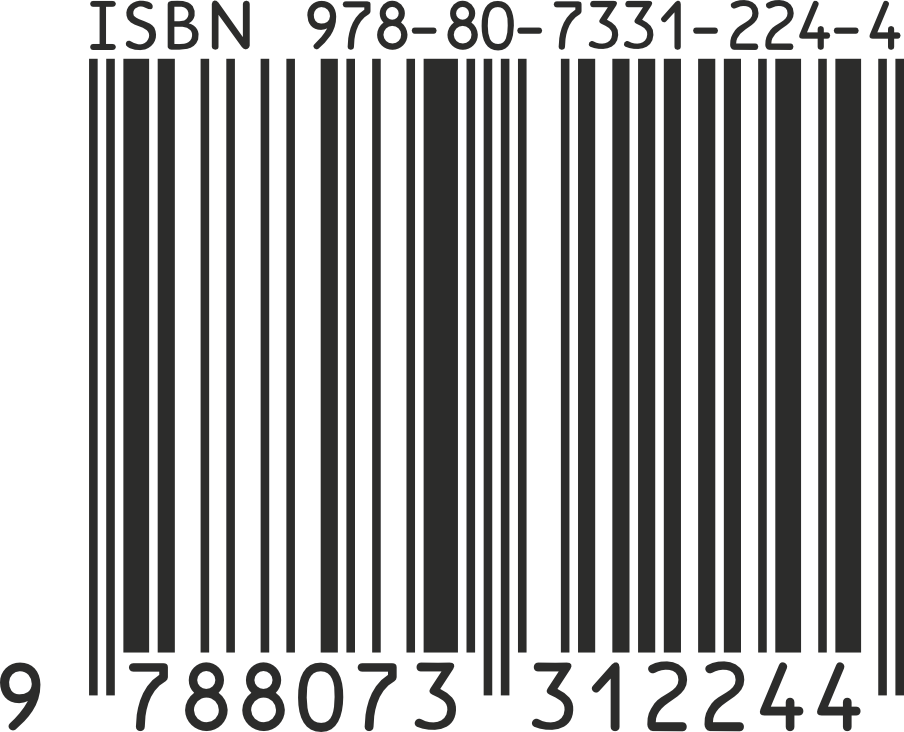
\includegraphics[width=0.25\textwidth]{imgs/barcode.png}
%\end{center}

\end{itemize}

\newpage


\oddilN{Poděkování}
Rád bych poděkoval všem lidem, kteří se podíleli na vzniku této publikace.

Nejprve děkuji Tomáši Pospiszylovi, vedoucímu této práce, za neúnavný dohled nad podobou následujícího textu.  Velmi rád bych poděkoval Miloši \nlb Vojtěchovskému za oponenturu práce, Andree Slovákové a Zdeňku \lnb Holému za konzultace a pomoc při vydávání publikace. Rovněž bych rád poděkoval Janě Křížové a Olze Stehlíkové za jejich korektorskou práci a~usměrnění příručky do mezí čitelnosti. Naposledy bych rád velmi \lnb poděkoval Janu Omastovi za podobu výsledného tisku.


\vspace{5em}

\begin{flushright}
{\em \footnotesize{-- Kryštof Pešek}}
\end{flushright}

\vfill

\newpage

\oddilN{Abstrakt}

Příručka {\em Processing Beta} je základním úvodem do jazyka {\em Processing}, ten byl navržen v akademických dílnách {\em Massachusetts Institute of Technology} k snazšímu a co možná nejsvobodnějšímu přístupu tvůrců -- obecně \lnb vza\-to -- všech netechnických oborů k pokročilým technologiím. Základ pro tuto příručku vznikl při sérii otevřených dílen o programování vedených Kryštofem Peškem na pražské FAMU.

Publikace vychází v tištěné podobě v době, kdy vývoj programovacího prostředí {\em Processing} opouští vývojovou fázi 1.0 a přibližuje se k fázi 2.0. Problematika, které se tento průvodce dotýká, je natolik základní, že se \lnb vztahuje na obě verze {\em Processingu}. Název příručky {\em Beta} by tedy měl co nejobecněji shrnovat základy všech dostupných verzí do dnešních dnů. 

Podobné příručky v posledních letech vznikly pouze v anglickém jazyce, např. Casey Reas a Ben Fry: {\em A Programming Handbook for Visual Designers and Artists} (2007), Ira Greenberg: {\em Processing Creative Coding and \lnb Computational Art}  (2007), Daniel Shiffman: {\em Learning Processing: A~Be\-ginner's Guide to Programming Images, Animation, and Interaction}  (2008), Tom Igoe: {\em Making Thinks Talk: Practical Methods for Connecting Physical Objects} (2007). V českém jazyce žádná podobná kniha doposud nevyšla.

Příručka by měla přiblížit, ve shodě s původním smyslem {\em Processingu}, technologie i netechnicky zaměřeným oborům, hlavně pak studentům výtvarných škol bez předešlé zkušenosti -- nebo jen s malou praxí s programováním.


Publikace byla zpracována jako diplomová práce studijního oboru \lnb Centra audiovizuálních studií na pražské FAMU a vznikla za podpory \lnb grantu {\em SGS AMU} (2011 -- 2012). 








\index{obsah}

\tableofcontents\thispagestyle{empty}

\pagestyle{empty}


\vfill
\chapter{O knize}



\vfill
\thispagestyle{empty}
%\begin{center}
%
\includegraphics[width=1\textwidth]{imgs/thePainOfFleetingJoy_1.jpg}
%\end{center}



\oddil{Na úvod}

\pagestyle{fancyplain}

Vážení čtenáři,

tato kniha by pro vás měla být povzbuzením při osvojování si vašeho prvního programovacího jazyka. Autor této publikace nepředpokládá žádnou vaši předchozí zkušenost s programováním. V případě, že již určitou praxi máte, některé kapitoly pro vás mohou být jednoduché. Kniha by vás měla postupně provázet při získávání dovedností programování stroje od základních výpočetních operací k tvorbě pokročilejších nástrojů.

Příručka je psána ve sledu, který bych uvítal, kdybych se sám měl učit programovat. Programování je bezesporu myšlenkově náročná operace. Mým záměrem je postupně tuto náročnost redukovat a proměnit psaní programu v lehkost.

Cestu k této zručnosti vám neumím jednoduše předat, pedagogický talent jsem nikdy nepocítil. Tato kniha by proto měla být odložena vždy, bude-li mít čtenář nutkání si něco sám vyzkoušet. To považuji za absolutně nejrychlejší a zároveň nejlepší způsob učení.

Proces tvůrčího programování obsahuje prvek intuice, která vychází podstatnou měrou ze zkušenosti. Pro podporu vaší intuice při psaní programu je nutné ovládnout základní jazyk natolik, abyste měli určitou jistotu. Přestane\-te-li se zabývat funkčností programu a získáte-li v ní jistotu, přijmete jazyk za vlastní nástroj, a pak můžete nechat hovořit právě vaši intuici. Intuici považuji za avantgardu logiky, protože je před ní vždy minimálně o krok napřed.

K vybudování intuice je především nezbytná schopnost pozorování. Samotná intuice nezmůže v komunikaci se strojem nic. Stroj neví, co počítá, ale dokáže spočítat i to, co sami nevíte.

Stroj je rychlý nástroj pro ověření vaší intuice a je zapotřebí být pozorný. Můžeme to nazvat experimentální přístup, výsledky by měly být vždy intui\-tivně a hlavně kriticky zkoumány. Zpětnou dekonstrukcí intuice, rozborem vaší jistoty, získáváte postupně dar rozumění věci. Dar je to danajský, rozumění je jen ustálená podoba znalostí, která musí být opět zpochybněna intuicí; nutno podotknout, že opakovaným prověřením se často jen více utvrzuje. 

Není-li tento programovací jazyk vaším prvním, prosím vás o trpělivost ohledně podrobností, do kterých v úvodu této knihy zabíhám. Šíře znalostí, které se mohou vyskytovat u potenciálních čtenářů tohoto průvodce, je pro autora první velkou neznámou.

V obou případech prosím o shovívavost ve způsobu popisu programovacího jazyka a prostředí {\em Processingu}. Sám jako samouk a člověk zaměřený zejména výtvarným směrem nemohu zaručit absolutní, stoprocentní \lnb a všeobecnou platnost všech tvrzení. Tímto vás tedy žádám o věcné podněty pro pozdější doplnění nebo přeformulování jednotlivých tezí.

Má snaha provést začínající i středně pokročilé uživatele programovacím jazykem bude vždy nedostatečná, berte tuto knihu, prosím, spíše jako průvodce nesnadnými začátky. Čtete-li knihu z jiných důvodů, než abyste se naučili programovacímu jazyku, pokusím se text proložit poznatky nabytými mojí několikaletou zkušeností se sdílením života se stroji. Dosta\-la-li se vám tato publikace do rukou jinou cestou, nebo dokonce náhodou či omylem, tedy věru netuším, co v ní dále najdete, a proto bych i vás rád pobídl alespoň k začtení se do světa skriptů a kódů.




\pododdil{Cíle příručky}

Cílem této knihy je provést uživatele-začátečníka sérií příkladů, které budou ilustrovat znalosti nezbytné k naprogramování jednotlivých stadií programu.

Prvním cílem této příručky je popsat základní terminologii používanou v jazyce {\em Processing}, tato pasáž je nezbytná pro další pokračování. Jestliže se cítíte v tento okamžik připraveni, můžete si rovnou nalistovat začátek průvodce \odkaz{Základní prostředí}.

Následující krok je pochopení datatypů a operací s nimi. Proměnné představují základní stavební jednotku {\em Processingu}, orientujete-li se například v jazyce {\em Java}, směle tento krok rovnou přeskočte, všem ostatním čtenářům ovšem stěžejní pasáž příručky důrazně doporučuji přečíst \odkaz{Logika programování}.

Dalším cílem publikace je uživatele {\em Processingu} uvést do zábavnější části programování: experimenty s obrazovým výstupem. Kapitoly týkající se základních kreslicích funkcí \odkaz{Zobrazení} jsou dobré pro naprosté začátečníky. Těm lehce pokročilým bych doporučil sekci věnovanou pohybu \odkaz{Pohyb} a kapitolu věnovanou interakci \odkaz{interakce}.

Všechny kapitoly postupně čtenáře vedou k osvojení si objektově orien\-tovaného jazyka. Zde se {\em Processing} stává opravdu mocným nástrojem. Pasáže v příručce věnující se podrobněji práci s objekty najdete zejména \lnb v pokročilejších kapitolách \odkaz{Uspořádání struktury programu}.

Všem čtenářům ovšem doporučuji alespoň si pročíst úvod, a tím získat základní představu o kontextu programovacího jazyka {\em Processing}.

\pododdil{Uspořádání informací}

Text je členěn do jednotlivých  kapitol a dále strukturován do dvou úrovní podkapitol. Pořadí kapitol by mělo odpovídat sledu informací nezbytných \\ k plynulému učení se programovacímu jazyku {\em Processing}.

Řazení a obsah jednotlivých kapitol vychází z mé vlastní zkušenosti. \lnb Z veliké míry koresponduje s podobnými průvodci, jež píšou samotní tvůrci a širší komunita uživatelů kolem programovacího jazyka {\em Processing}.

Zvolená forma textu odpovídá ověřeným postupům. Následující text \lnb bude podléhat určitým zákonitostem. V knize se objeví několik typů textu, které budou vždy odlišeny formou zápisu.

\newpage
\pododdil{Pravidla formátování v knize}

Pravidla jsou následující:

\begin{itemize}

\item[Obyčejný text:]
popis ve formě klasického textu

\item[\texttt{\small kód:}]

\begin{lstlisting}
/**
* Barevny text v sedem ramovani bude znacit
* strojovy kod ve forme ktera je srozumitelna
* Processingu.
*/

boolean pravda = true;

\end{lstlisting}


\item[\klavesy{CONTROL + T}:]
klávesové zkratky, které jsou psány \uv{verzálkami}

\item[\slovnik{GNU / GPL}:]
výrazy a pojmy, jejichž definici můžete nalézt ve slovníku na konci knihy

\item[\vyraz{boolean}:]
jednotlivé příkazy a oficiální příkazy {\em Processingu}, které jsou zároveň zařazeny do slovníku

\item[{\em promenna}:]
proměnné a názvy použité v kódu, které bude potřeba dovysvětlit \lnb v textu


\item[cvičení:]
Pomocí cvičení a otázek si můžete kontrolovat v průběhu textu nabyté znalosti. Bublina bude vždy značit důležité informace, například ty, které si musíte zapamatovat, abyste se mohli orientovat \lnb v následujícím textu.\bublina{Zapamatujte si, prosím, jak budou znázorněna cvičení.} 

\end{itemize}





\newpage
\chapter{Od textu k~obrazu}

\oddil{Krajiny a světy}

Robert Hodgin, také známý pod pseudonymem {\em flight 404}, zůstává jednou z oslavovaných ikon processingové komunity. Jeho práce s vizualizacemi je vždy velmi dynamická a technicky obdivuhodná.

Hodgin pracuje s jazyky {\em Processing} a {\em Cinder}\index{Cinder}. V obou případech skrze tato prostředí ovšem programuje přímo aplikaci {\em OpenGL}, která zprostředkovává pokyny samotnému grafickému jádru.

\vfill
\newpage

\begin{centering}
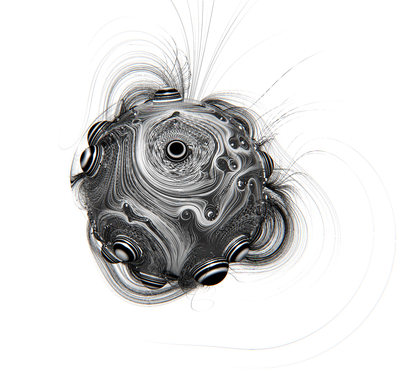
\includegraphics[width = 1\textwidth]{imgs/hogin.png}
\end{centering}

Ilustrace pochází z Hodginovy\index{Hodgin, Robert}\index{flight404} grafické práce, která byla vybrána jako jedna ze 42 výtvorů do prvního vydání knihy {\em Written Images}.

Publikace je kurátorským projektem a samostatným výtvarným počinem dánského tvůrce Marcina Ignace. \index{Ingac, Marcin}

První výtisk knihy byl vydán v roce 2011, kniha byla zpracována softwarem {\em Processing}. Jde v podstatě o konceptuální dílo, automatizací vychází každý výtisk s posunem o jedno okénko, a tím ilustruje ducha generativní tvorby.

\vfill

\begin{centering}
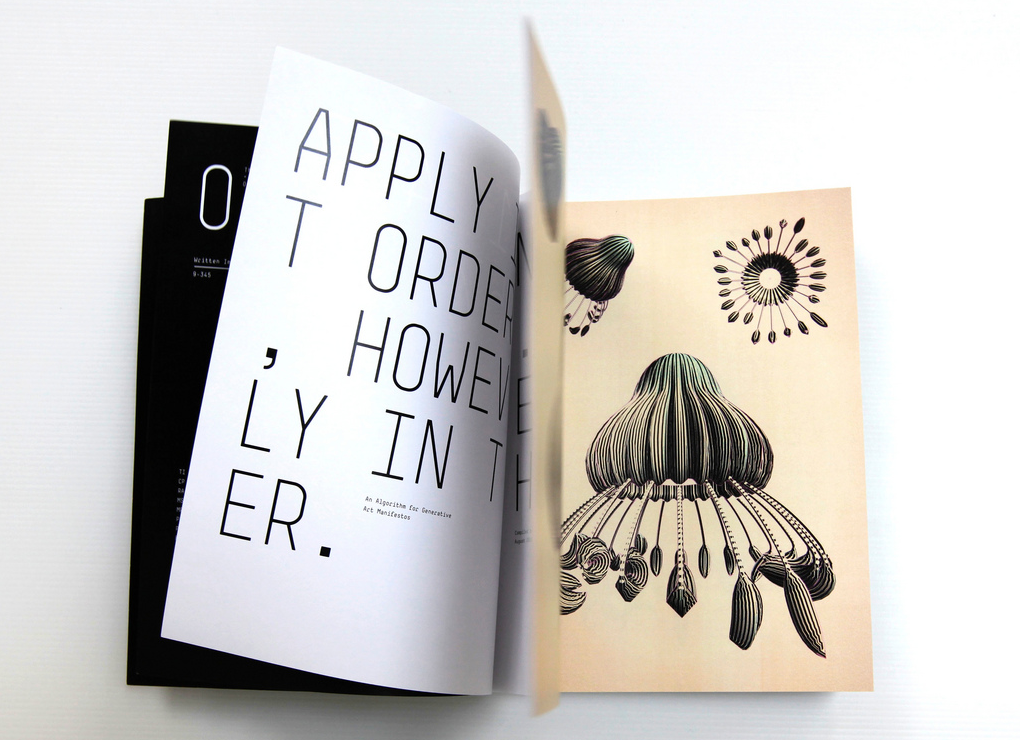
\includegraphics[width = 1\textwidth]{imgs/writtenimages.png}
%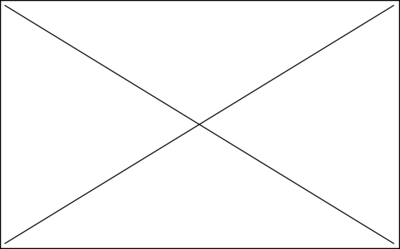
\includegraphics[width = 1\textwidth]{imgs/neznamy.png}
\end{centering}

Kniha obsahuje generativní obrazy následujících umělců:
{\em 
386dx25, \lnb Antoni Kaniowski, Ariel Malka, Carl-Johan Rosén, Casey Reas, clone, \lnb David Bollinger, David Bouchard, e m o c, flight404, Golan Levin, \lnb Jonathan McCabe, Jörg Piringer, Julien Deswaef, Kim Asendorf, kraftner, Leonardo Solaas, Lia, Luke Sturgeon, Marcin Ignac, Marius Watz, Michael Zick Doherty, Mitchell Whitelaw, Moka, Nervous System, Oliver Smith, \lnb paolon, Perceptor, rhymeandreason, Ricard Marxer, Roberto Christen, Rui Madeira, Ryan Alexander, Ryland Wharton, Sansumbrella, sojamo, \lnb Stefano Maccarelli, Szymon Kaliski, Victor Martins, W:Blut, William \lnb Lindmeier, zenbullets.} 




\newpage
\oddil{Toxilibs}


\begin{center}
%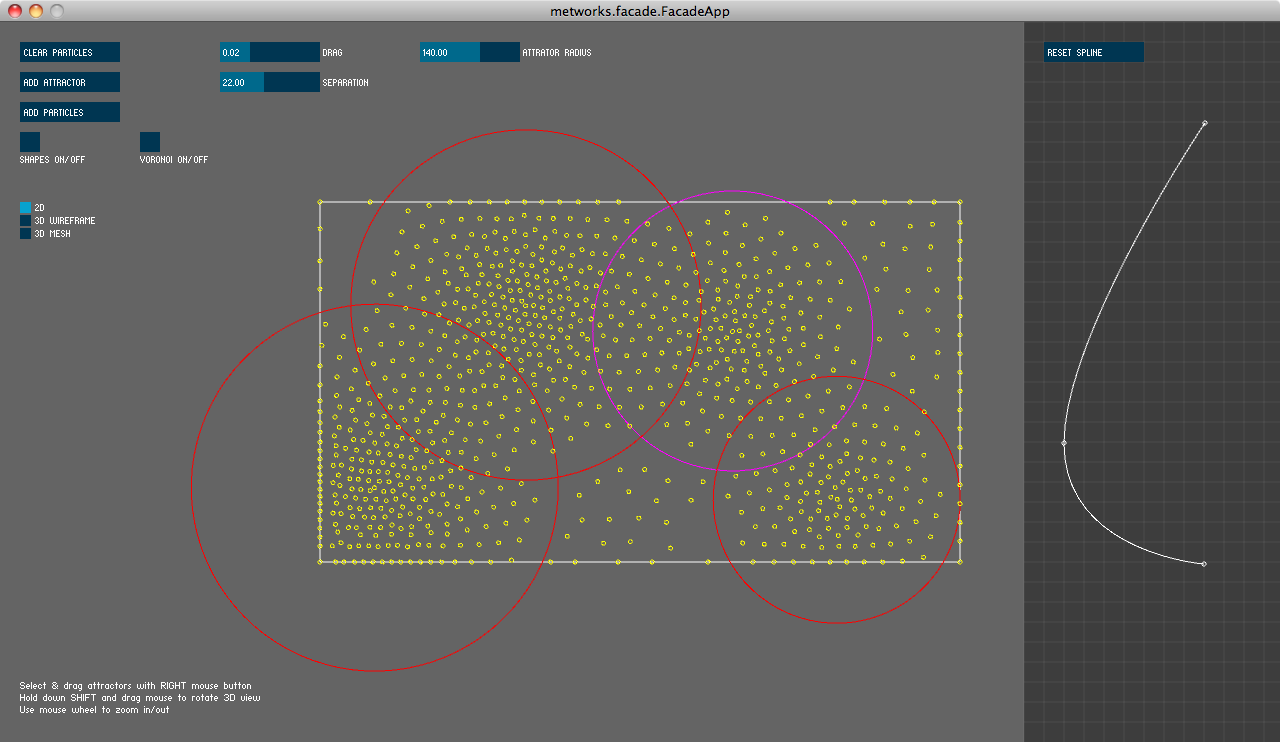
\includegraphics[width = 1\textwidth]{imgs/facade-1.png}

\includegraphics[width = 1\textwidth]{imgs/moebius.png}

\end{center}


Karsten Schmidt působí v processingové komunitě dlouhodobě a je více znám pod pseudonymem {\em Toxi}. Schmidt je autorem sady rozsáhlých knihoven nazvaných souhrnně {\em Toxilibs}. \index{toxilibs} Jeho tvorba je zaměřena technicky na vývoj samotných knihoven, tedy jednotlivých modulů rozšiřujících funkce {\em Processingu} \odkaz{Knihovny}. V případě knihovny {\em Toxilibs} například rozšířením o funkce pro konstrukci trojdimenzionálních objektů.


\begin{center}
%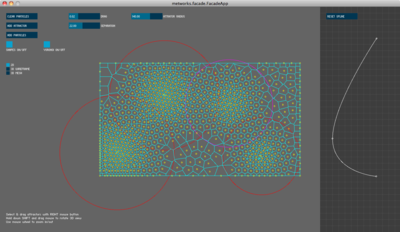
\includegraphics[width = 0.5\textwidth]{imgs/facade-3.png}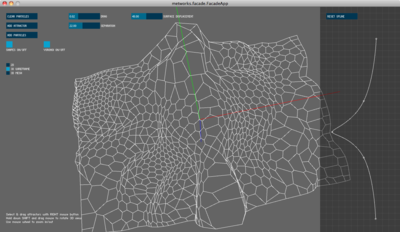
\includegraphics[width = 0.5\textwidth]{imgs/facade-5.png}
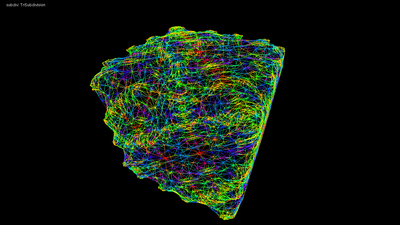
\includegraphics[width = 0.5\textwidth]{imgs/laplacian.png}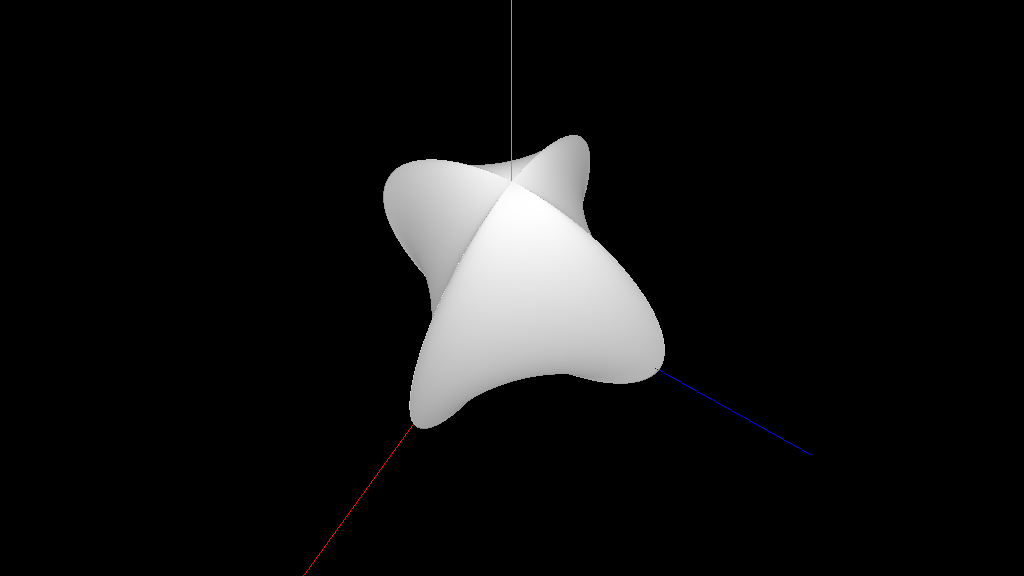
\includegraphics[width = 0.5\textwidth]{imgs/smooth.png}


\end{center}

Schmidtova práce vyniká zejména pro možnost recyklovatelnosti a další užitné hodnoty samotného kódu. Schmidtovy algoritmy jsou propracované a matematicky pokročilé. Práce Karstena Schmidta dobře ilustruje podstatu komunitní práce ve formě knihoven, které volně cirkulují mezi uživateli \lnb a jsou volně využívány v duchu svobodného softwaru. \index{Schmidt, Karsten}






\begin{center}
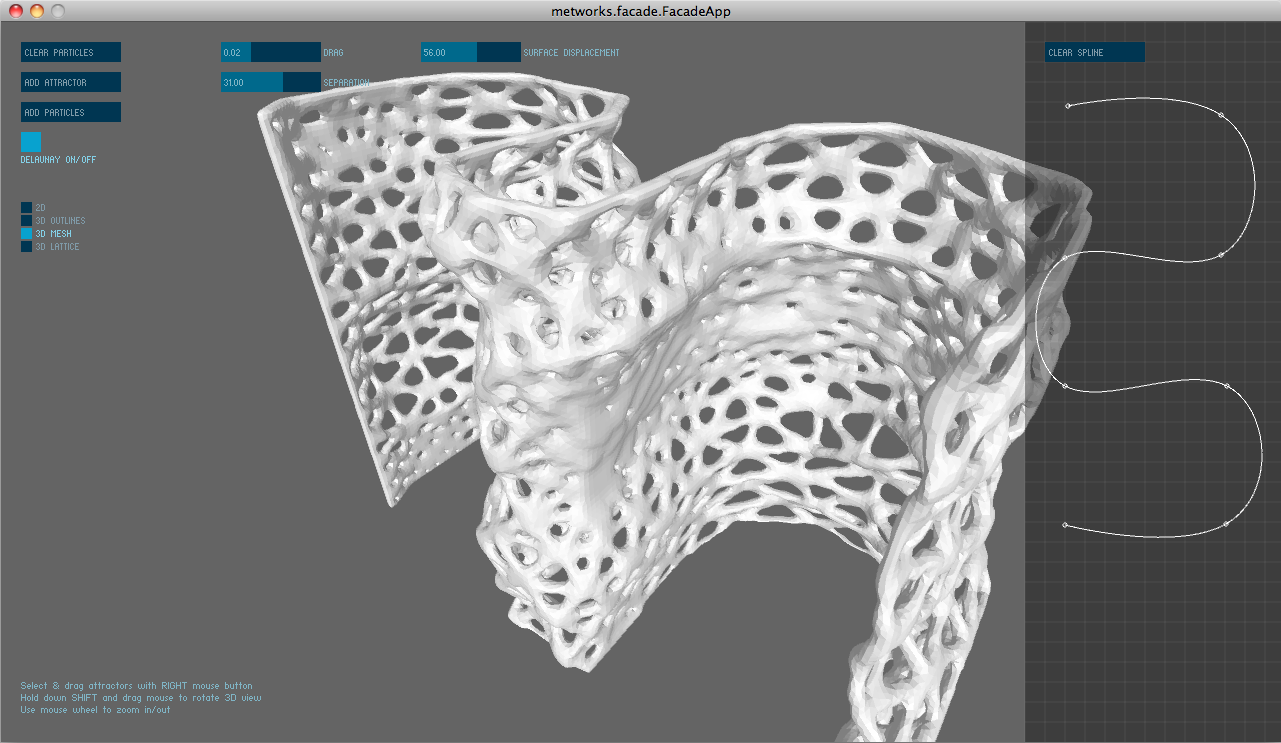
\includegraphics[width = 1\textwidth]{imgs/facade-7.png}
%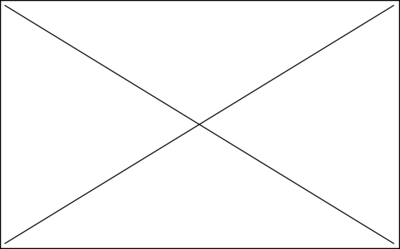
\includegraphics[width = 1\textwidth]{imgs/neznamy.png}

\end{center}


Tvorba Karstena Schmidta \index{Schmidt, Karsten} se dá generalizovat jako užitá nebo aplikovaná. Pomocí bohaté zásoby vlastního softwaru, veliké zdatnosti a technické inovativnosti Karsten Schmidt svým softwarem plynule navazuje na potřeby architektů a inženýrů.



\oddil{Local Bilateral Symmetry}


Pozoruhodné algoritmy Jonathana McCaba vynikají svou spektakulárností, která je založena na podrobné studii a rozkladu Turingových vzorců. Jednotlivé variace téhož algoritmu vytvářejí struktury, které se vzdáleně podobají uspořádání organických materiálů v kostech nebo jiným přírodním vzorům.\index{McCabe, Johnatan}


\begin{center}
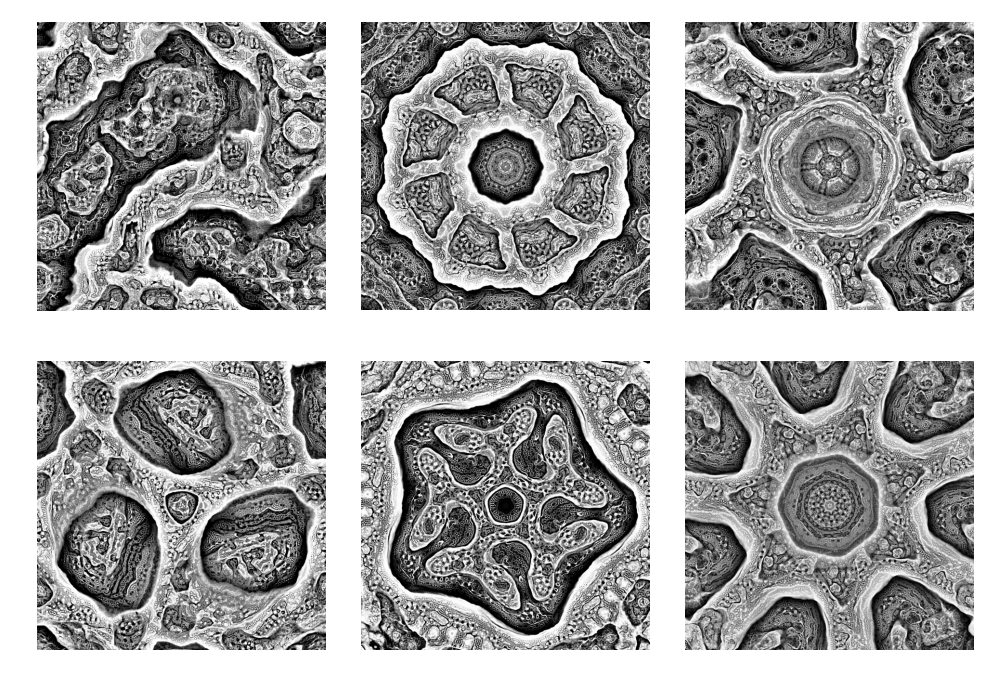
\includegraphics[width = 1\textwidth]{imgs/mcCabe1.png}
\end{center}

I když se to zprvu nabízí, \index{McCabe, Johnatan} McCabovy obrazy se nedají posuzovat pouze výtvarně. Nejvíce pozoruhodné jsou způsobem svého vzniku. Obrazy přímo odkazují na výzkum Alana Turinga\index{Turing, Alan}, konkrétně na text vydaný v roce 1952 s názvem {\em The Chemical Basis of Morphogenesis}, který pojednává o vlivu chemických sloučenin na uspořádání růstu tkáně vícebuněčných organismů. Turing podobnou difuzi prvků v textu rozpracoval matematicky a po téměř padesáti letech na bázi původních algoritmů vznikají tyto obrazy. Podobnost v uspořádání lze nalézt například ve snímcích tkáně pod elektronovým mikroskopem, a i když se jedná o ryze výtvarnou interpretaci algoritmu, může dovést k zamyšlení i vědecké kruhy.


\begin{center}
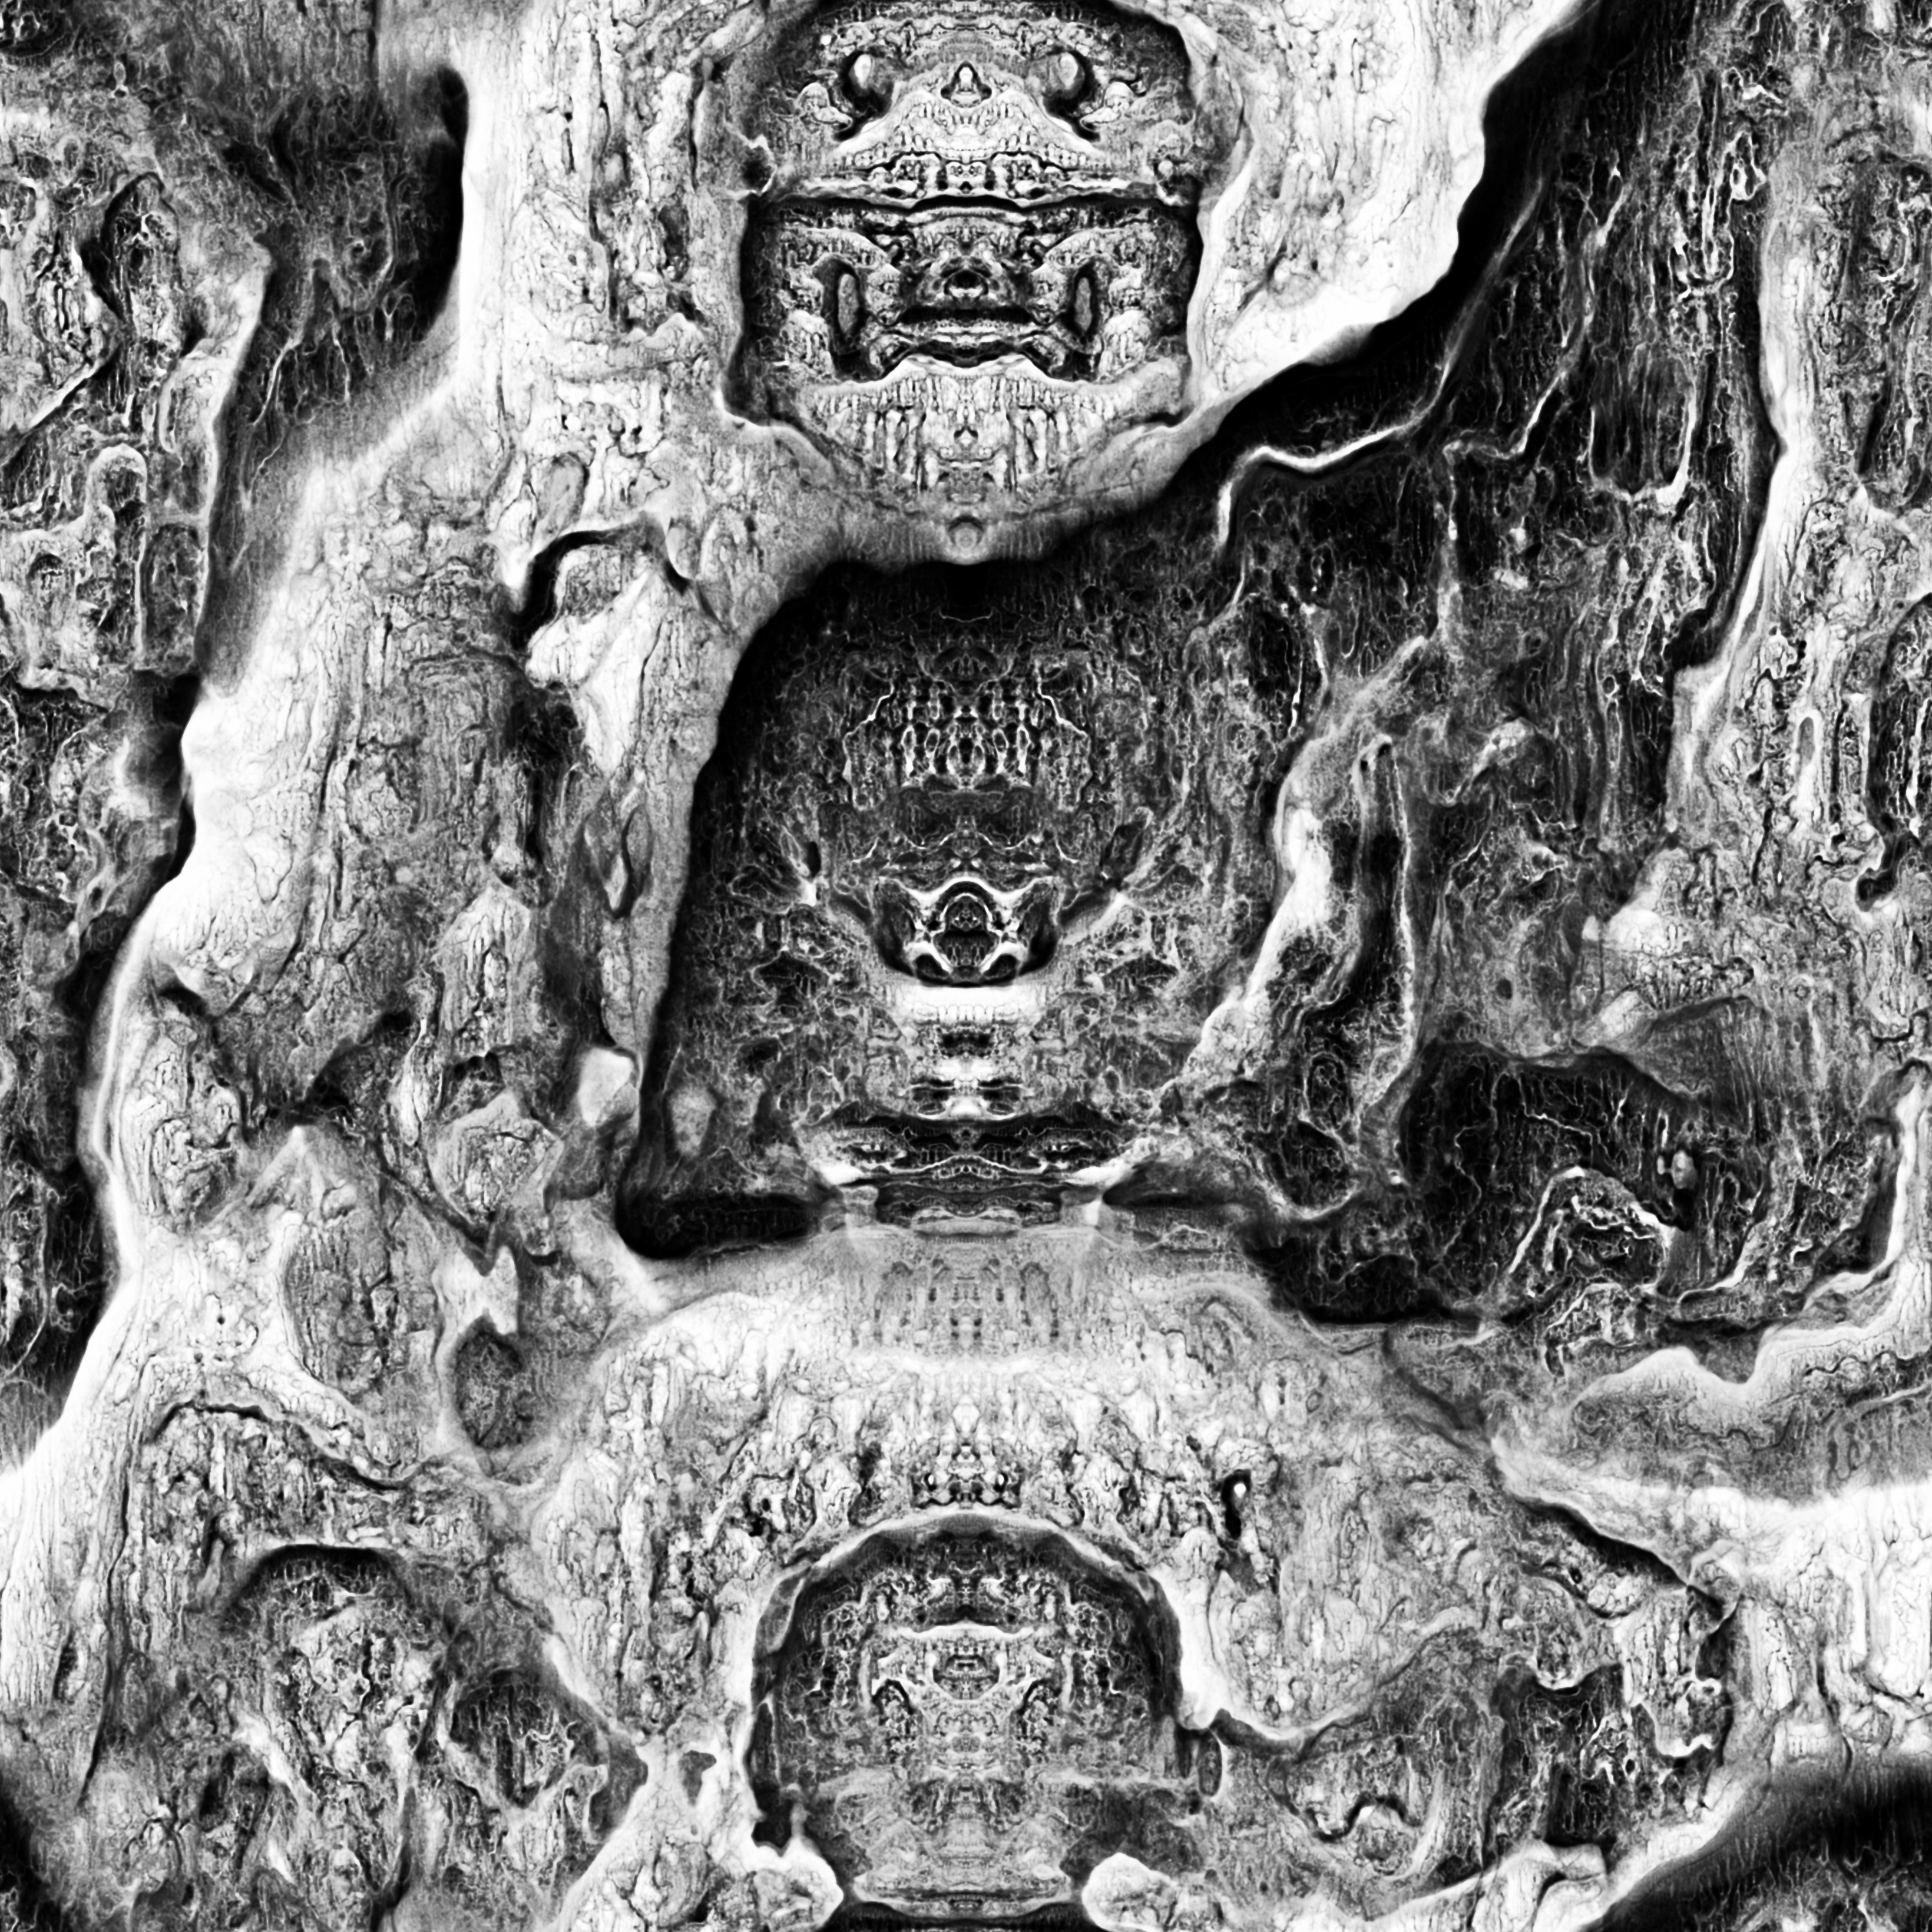
\includegraphics[width = 0.95\textwidth]{imgs/turingpattern.jpg}
\end{center}

\ 







 



%\end{comment}




\chapter{Dobré zdroje v~začátcích}

\oddil{Síť}

Autor knihy předpokládá, že čtenář má přístup ke globální síti internet.

Nejlepší referencí pro práci s {\em Processingem} zůstává tato síť. {\em Processing} byl vyvinut síťovou komunitou a je také v síti nejlépe zdokumentován. Existuje několik dobrých obecných stránek s průvodci. Za všechny lze jmenovat domovskou stránku projektu {\em processing.org}. Zde naleznete téměř vše, co byste mohli potřebovat. Nacházejí se zde zdokumentované veškeré příkazy {\em Processingu}. Je zde i záložka {\em Learning} s jednotlivými průvodci různých oblastí.

Nejadresněji se vám dostane pomoci prostřednictvím webových fór nebo \index{IRC} IRC-kanálů. Na fórech se již řešil téměř jakýkoli problém, stačí proto vyhledávat klíčová slova konkrétního dotazu a velmi rychle byste měli nalézt řešení.
 
   Na síti je dále obrovské množství uživatelů volně sdílejících své programy včetně zdrojových kódů. Nejpočetnější komunita sídlí zřejmě na portálu {\em openprocessing.org} založeném a spravovaném \index{Ascioglu, Sinan} Sinanem \lnb Asciogluem.
   
Veškerá dokumentace je v angličtině včetně webových fór i dalších knih o programování. Nemáte-li problém s anglickým jazykem, míst \lnb k zdokonalování se v {\em Processingu} bude vždy dostatek. \bublina{Doporučuji se nejprve seznámit s projekty na inter\-netu, získáte tím představu o tom, \lnb k čemu se vlastně Processing využívá.}


\oddil{Examples, příklady přímo v Processingu}

Tato pomoc je vždy po ruce. {\em Processing} je navržen k výuce a je připraven poskytovat pomoc ze své podstaty. Přímo do aplikace {\em Processingu} jsou naimplementovány základní postupy programování. Témata jsou pokryta od základních operací až po pohyb v trojdimenzionálním prostoru nebo manipulaci s pixely. \index{Processing Examples}

Příkladů je na webu dostatek a jsou přehledně uspořádány. Vřele doporučuji si je čas od času projít.

Ke všem příkladům se dostanete z {\em Processingu} skrze nabídku {\em File $\rightarrow$ Examples} \odkaz{Základní prostředí}.

\oddil{Knihy a průvodci}

Ano, jednoho průvodce právě držíte v rukou (nebo čtete na obrazovce). \lnb V minulosti vyšla bezmála desítka podobných knih na stejné téma. Jsou bezesporu obsáhlejší, než kdy měla tato příručka v úmyslu.

Z nich bych vám nejvíce doporučil základní příručku od samotných tvůr\-ců {\em Processingu} Caseyho Rease a Bena Frye \index{Reas, Casey}\index{Fry, Ben}nazvanou {\em Processing: A~Programming Handbook for Visual Designers and Artists} (2007). A~rozhodně pak knihu Daniela Shiffmana\index{Shiffman, Daniel} {\em Learning Processing: A Beginner's Guide to Programming Images, Animation, and Interaction} (2008). Je jednou z~velmi podrobně napsaných knih o {\em Processingu}.

Knihy jsou cenově vcelku dostupné a dají se opatřit přes internet. Rozhodně bych to doporučoval všem, kteří  potřebují mít opravdu dobrou dokumentaci vždy při ruce. V neposlední řadě bych také upozornil na to, že koupí knihy podporujete tvůrce svobodného softwaru, a tím potažmo i svobodný software jako takový \odkaz{Otevřenost softwaru}.

\oddil{Experiment}

Nejdůležitějším zdrojem vašich vlastních zkušeností bude vždy samotné experimentování s programováním. Na tuto část kladu největší důraz \lnb a v průběhu této knihy to i několikrát zopakuji: je vždy dobré odložit knihy a reference a odvážit se do neznámých vod. Zkušenost, kterou takto naberete, bude vždy ta nejhodnotnější. Nebojte se proto sami experimentovat \odkaz{Empirický přístup k programování}. \bublina{Příštích několik kapitol se věnuje obecnějším úvahám o programovacích jazycích, již nyní si můžete Processing nainsta\-lovat.}

%\part{Programovací jazyky}

\newpage
\chapter{K čemu slouží programovací jazyk?}

\oddil{Počátky programovacího jazyka}

Výchozím bodem v tvorbě počítačové logiky, jak ji známe dnes, byla přirozená lidská komunikace v podobě řeči. Člověk používá jazyk  a při tvorbě zcela nového systému pravidel zákonitě sahá po známém prostředku.

Na počátku programování ale nebyl lidský jazyk. Se stroji se v jejich raných fázích vývoje hovořilo čistě strojovým jazykem, v podobě číselných řad nebo později holého strojového kódu, který přešel na logiku pokročilejších obvodů. Programovací jazyk se objevil již v padesátých letech minulého století a osvědčil se jako prostředek pro člověka, který začínal být limitován oproti kapacitě stroje schopného obsáhnout složitější úlohy. Řešením pro vzrůstající složitost logiky programů se stala lidská řeč.

Řeč se v počátcích tvorby struktur pro program jevila jako člověku nejpřirozenější řešení. Velmi brzy tvůrci zjistili, že pomocí jazyka lze sice definovat složitý problém pro člověka, vyvstává tím ovšem problém definovat význam takového jazyka pro stroj.

Počítačový jazyk není jeden, počítačových jazyků jsou celé rozvětvené rodiny. Konceptů, jak lépe hovořit srozumitelně pro člověka a zároveň ke stroji, je celá řada, žádný z nich nedokáže plně kopírovat lidský jazyk v jeho přirozené struktuře. Důvodů je několik, jeden z nejpodstatnějších je fakt, že lidská řeč neodpovídá organizaci ve struktuře stroje prostě proto, že člověk své řeči sám nerozumí natolik, aby popsal všechny její zákonitosti logickou cestou.

\pagebreak

Jednoduše řečeno, lidský jazyk není popsán tak dokonale, abychom ho byli schopni vysvětlit stroji. Pokusy o průnik lidské řeči a logického \lnb obvodu sahají do absolutních počátků interakce člověka se strojem a představují pro tvůrce strojů závažný problém. Tento problém v padesátých letech minulého století definoval Alan Turing, jeden ze zakladatelů dnešní výpočetní techniky. Alan Turing spolu s Gordonem Wechmanem stáli \lnb v~době druhé světové války u vývoje stroje k rozkrývání německých šifer nazvaného {\em Bomba (The Bomb)}. Alan Turing v poválečné éře definoval formální rámec počítače, jak jej známe dnes. Koncepce později nazvaná Turingův stroj vycházela zejména z matematických potřeb a jednalo se o~snahu vytvořit kompletní výpočetní jednotku schopnou řešit veškeré známé matematické operace. \index{Turing, Alan} \index{Bomb, The}


Je pozoruhodné, že Alan Turing se již v raných stadiích vývoje počítačů zabýval takzvanou umělou inteligencí. Z toho je zřejmé, že stroje podobné počítačům se od počátku svého vzniku připodobňují struktuře lidského uvažování. Alan Turing sestavil pro stroje známý experiment nazvaný Turingův test, jenž měl prověřit schopnosti stroje replikovat lidské chování. Není náhodou, že prostředkem pro komunikaci v testu byla zvolena právě řeč. Test spočíval v modelové situaci stroje schopného napodobit lidskou komunikaci tak dokonale, aby člověk nebyl schopen rozeznat, že komunikuje se strojem. Zajímavá na této definici lidské inteligence je zejména její vágnost, která v podstatě ilustruje míru porozumění logického uvažování lidské mysli jako takové.

K tomu, abychom sdělili informaci, používáme jazyk. Jazyk musíme umět přizpůsobit tomu, aby informoval, sdělil jistou skutečnost -- myšlenku sdělovanému subjektu. Jazyk má nutně několik úrovní, zdaleka ne všechny jsme schopni reflektovat. Logicky popsaným jazykem a vnitřně uceleným systémem jsme schopni vysvětlit pouhý fragment skutečnosti.

Programovací jazyk je prostředek pro zápis algoritmů, jež mohou být provedeny na počítači. Zápis algoritmu ve zvoleném programovacím \lnb jazyce se nazývá program.





\oddil{Jednoduchý programovací jazyk}

Snaha o zpřístupnění programování širší veřejnosti dala již na konci \lnb 20. století vzniknout rodině jazyků, které jsou patřičně zjednodušeny tak, aby je mohli obsluhovat i laici.

Zjednodušit programování je odpověď na situaci, kdy programovací jazyky vytvářeli především lidé se zvláštním nadáním pro ryze technické uvažování. Pro technické myšlení nemá každý člověk správné predispozice. Programování v současnosti znamená zejména určitý stupeň svobody při komunikaci se strojem.

K míře svobody, která má své silné kritiky\poznamka{Včetně mne samotného.}, se nyní nechci vyjadřovat, ale zjednodušeně z pohledu pouhého uživatele, který používá daný nástroj, schopnost programovat činí z uživatele již potenciálního tvůrce vlastních nástrojů.

Hovořím-li o stroji, mám na mysli spotřební počítač. Termín \slovnik{stroj} po\-užívám záměrně pro zdůraznění jisté formy strojového přemýšlení v historickém kontextu.

Nástroje jsou pak programy zkonstruované pro jistou činnost. Nástroj je obvykle vyvíjen za jedním účelem, který plní uživatelsky co nejpřívětivější cestou. Tato cesta je pro uživatele schůdná a nabízí mu standardní škálu dovedností nástroje.

Aniž bychom si to často uvědomovali, současná vizuální kultura je ovlivněna těmito nástroji daleko více, než je na první pohled zřejmé. Technické možnosti jsou současným tržním hladem po inovaci patentovým systémem vlastněny a proměňovány ve zboží. V této situaci je důležité znát nástroje i jejich vznik pro reflexi nebo kritiku v širších souvislostech.

Tato kniha je spíše nežli jednomu nástroji věnována programu pro tvorbu takových nástrojů. Jak již vyplývá z této definice, použití {\em Processingu} není limitováno jen úhlem pohledu autora tohoto textu. Návod by se měl stát spíše pobídkou k co nejrozmanitější tvorbě vlastních nástrojů sloužících opět k co možná nejširší škále možných účelů.

{\em Processing} vychází z koncepce snadného přístupu k programování. \lnb Za běžných okolností by se vnímavý člověk měl být schopen naučit jednoduché struktuře programu a vytvořit vlastní program v průběhu několika dní. Na druhou stranu, právě predispozice našeho uvažování jsou \lnb natolik rozmanité, že takovou prognózu nelze brát jinak než jen jako orien\-tační.




\oddil{Dokonalost jazyka}

Co je to dokonalý jazyk? Obecně je zapotřebí říci, že absolutně dokonalý jazyk neexistuje. Jazyk si můžeme představit jako systém vzájemných vztahů, který je schopen popsat jednotlivé symboly nebo objekty. Symboly můžeme nazvat předměty, tyto předměty dále mají své vlastní hodnoty \lnb a vlastnosti. Jazyk kromě definic takových vlastností operuje a popisuje jednotlivé jevy a vztahy mezi těmito předměty. Jednodušší popis jazyka je \lnb v pojetí výpočetní techniky určitý ucelený systém schopný popsat rozmanité problémy řešitelné strojem.

Co předem činí jakýkoli jazyk absolutně nedokonalým, je fakt, že jakýmkoli jazykem nedokážeme vyjádřit původ jazyka, tj. jeho strůjce, člověka. Jazyk použitý pro instruktáž stroje je vnitřně konzistentní a funguje logicky hermeticky, tedy nepřipouští jiný než jeden výklad konkrétního textu. Pojetí dokonalosti jazyka ve smyslu vnitřní logické konzistence je naprostou nezbytností v pojetí interpretace strojem, na druhou stranu téměř nepřekonatelnou překážkou v případě abstraktnějších úvah o programování jako takovém.

Použiji zde pro názornost rozdíl programovacího jazyka a jazyka českého. Český jazyk je jazykem organicky ustáleným po staletích užívání. Jazyk, jak ho známe, slouží ke komunikaci mezi lidmi, lze jej tedy použít například pro popis krajiny. Přestože k dokonalému popisu krajiny můžeme stěží dojít, slovy, která se opírají o určitou sdílenou zkušenost, lze poměrně dobře přiblížit určitý obraz věcí.

Kdybychom se pokusili pro popis krajiny použít jazyk programovací, dostaneme se velmi rychle do nesnází. Programovací jazyk není jazykem určeným pro předávání informací mezi lidmi, ale pro komunikaci člověka se strojem. Jeho vnitřní logická konzistence, tvrdá logická struktura, která nedovoluje v jeden okamžik jinou než jednu interpretaci, je jeho velikou předností při definici exaktních parametrů. Podobnost s řečí spočívá ve vazbě slov, která reprezentují jednotlivé hodnoty a operace. Hlavní odlišnost je v jeho syntetickém původu, jedná se o jazyk umělý. Programovací jazyk je přednostně zkonstruován pro definici známého a pochopeného. \lnb V případě neznámých nebo nepoznaných veličin je programovací jazyk víceméně k ničemu. 

Chceme-li komunikovat se strojem, musíme tedy svůj způsob vyjadřování přizpůsobit logicky dokonalému jazyku -- vnitřní logice fungování stroje. Počítač není navržen k tomu, aby něčemu rozuměl. Počítač je na-vržen k řešení jasně definovaných otázek. Tato příručka se pokusí srozumitelnou formou popsat jeden z možných způsobů, jak si takový jazyk osvojit a potažmo způsob uvažování, který vede k jasné definici problému. Hovoříme-li o programování, máme na mysli proces tvorby jisté logické struktury. Osvojení si programování spočívá ve schopnosti definovat problém nebo jasně formulovat otázku tak, aby na ni stroj mohl odpovědět.

Vtip spočívá v tom, že ovládneme-li formálně jazyk určený stroji, můžeme prostřednictvím tohoto stroje hovořit i ke člověku, tj. popisovat i pocity z rozkvetlých luk.

\oddil{Volba vhodného jazyka}

Ve výpočetní technice se nachází celá škála programovacích jazyků i prostředí. Tyto jazyky mají svoji genezi a byly historicky vyvíjeny především počítačovými odborníky. Jejich dokonalost lze těžko ocenit z vnějšího pohledu, a to právě z důvodu jejich konstrukce, která odpovídá a částečně podléhá určitým účelům, ke kterým byly tyto jazyky původně navrženy. Celistvý pohled na vývoj programovacích jazyků zde není možné obsáhnout. Programovací jazyk dle historického vývoje můžeme rozdělit na dvě skupiny, jazyky imperativní a objektově orientované. Toto základní rozdělení programovacích jazyků popisuje dva rozdílné přístupy v popisu událostí. 

{\em Processing} se svou stavbou na základech {\em Javy} řadí k objektově \lnb orientovaným jazykům. Programovací jazyk {\em Java} je relativně mladým jazykem. Historie tohoto jazyka sahá přibližně do roku 1995. Mezi jeho hlavní výhody, ze kterých i {\em Processing} velmi těží, jsou zejména důraz na multiplatformnost a relativní jednoduchost syntaxe. Příbuznými jazyka {\em Java} jsou další objektově orientované programovací jazyky jako {\em  C++}, {\em  Perl}, {\em Object Pascal}, {\em Visual Basic}, {\em C\#}, {\em PHP}, {\em Python}, {\em Ruby}, {\em Smalltalk}, nebo {\em Lisp}. \index{programovací jazyky}

Rozdíl mezi imperativním pojetím programování a objektově orientovaným pojetím spočívá především v logice kódu a jeho následném uspořádání. Imperativní jazyk se dá považovat za předchůdce objektově orientovaného pojetí. Nedá se obecně říci, který přístup je výhodnější, jedná se \lnb o dvě rozdílná paradigmata. Dnes mezi nejpoužívanějšími programovacími jazyky masivně převládá objektově orientované paradigma.

Rozdílné pohledy lze ilustrovat na popisu nějakého jevu. Jev se dá popsat různými způsoby. Jedna perspektiva bude více hovořit o aktérech jevu, ty rozdělí do objektů, jejich vlastností a možností. Druhá perspektiva popíše celistvou situaci jako sérii událostí, které je možné v tomto pořadí kdykoli zopakovat.


V posledních přibližně dvaceti letech se mezi programovacími jazyky postupně objevuje tendence po větší srozumitelnosti a potažmo zjednodušení programování jako takového. Programování v této koncepci již není jazykem odborníků, ale je demokraticky přístupné širší veřejnosti z rozmanitých -- prioritně netechnických oborů. \index{objektově orientované jazyky}

Tato tendence postupně dala vzniknout celé rodině programovacích jazyků, které se snaží přiblížit potenciál výpočetní techniky netechnickým oborům, v neposlední řadě i oborům výtvarným. V technických kruzích je ovšem již sama disciplína psaní programů považována za tvůrčí činnost. \lnb V pojetí výtvarného umění dnes převažuje pohled na programování jako na velmi technickou zdatnost, rigidní a notně limitovanou.

Jazyk, který je nutně limitován svou nezbytnou formální dokonalostí, ovšem nemusí nutně limitovat svého uživatele ve sdělení. Uživatel se musí  k uskutečnění takové zdárné komunikace přizpůsobit stroji.


\oddil{Proč zrovna Processing?}

{\em Processing} je vhodný nástroj pro první experimenty s programováním \lnb z několika důvodů.

Prvním důvodem je jednoduchost pro uživatele, {\em Processing} se snaží začátečníky co nejméně zatížit zbytečnými informacemi. {\em Processing} prezentuje programování jako přístupnou a zvladatelnou schopnost. Dosahuje \lnb toho především rychlou odezvou vizuálního prostředí. Jednoduše řečeno, \lnb v momentu, kdy spustíme kód, vidíme okamžitě jeho výsledek. Taková ilus\-trativnost je v začátcích podle mého názoru téměř nezbytná.

V {\em Processingu} lze velmi krátkým kódem programovat sofistikované programy. Pro příklad zde uvedu soutěž nazvanou {\em Tiny Sketch} pořádanou portály {\em rhizome.org} a {\em openprocessing.org}. \bublina{Máte-li počítač u~sebe a~jste-li připojeni k~internetu, vřele doporučuji si nyní projít aktuální podobu stránky {\em openprocessing.org}.} {\em Processing} dokáže být natolik \lnb úsporný, že pomocí maximálně dvou set znaků byli tvůrci schopni naprogramovat svébytné programy.

\vfill

\begin{center}
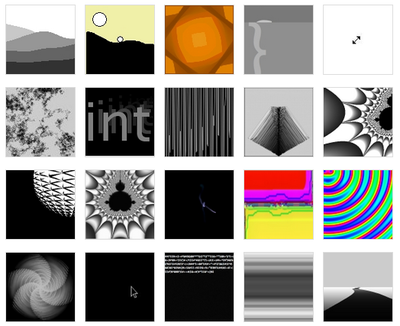
\includegraphics[width = 1\textwidth]{imgs/tinysketch.png}
\end{center}



Snad největší předností pro začínající programátory je výtečná dokumentace a velmi přívětivá komunita lidí poskytující neúnavně rady začátečníkům.


\oddil{Tvorba softwaru}

Programy jsme v současnosti zvyklí spíše využívat než sami vytvářet. Tvoření programu je náročný proces a tvorba uživatelsky přátelského prostředí je velmi složitá.

{\em Processing} se svým způsobem neliší od žádného jiného programu, který běžně využíváme. Jde o sadu příkazů a programovací prostředí, které nám dovoluje určitou formou vytvářet svébytný program. I když se již jedná o~programování, nelze jej běžně zaměňovat s klasickou tvorbou vyspělého nástroje.

Zde si musíme uvědomit, že náš potenciální výsledek -- program bude vždy spíše banální v porovnání například se samotným prostředím {\em Processingu}. Processingový kód je výčet všech možností, které můžeme při tvorbě našeho programu využít. Obecně se dá říci, že {\em Processing} je nástroj pro tvorbu speciálních nástrojů. Výsledek našeho programování bude vždy pravděpodobně obsahovat poměrně větší část {\em Processingu} samotného.

Je dobré od začátku pochopit, k čemu lze {\em Processing} využít a k čemu jej opravdu využívat chceme. {\em Processing} se především hodí k rychlé tvorbě programu, ověření teze nebo spontánního nápadu. Pro podobné programování se také vžil pojem \uv{rapid engineering}. Tvorba dospělejších nástrojů není sice nemožná, obecně ale platí, že {\em Processing} bude svými zkrácenými zápisy a jednoduchostí prostředí velmi nápomocný v začátcích. 

{\em Processing} se svou konstrukcí zejména hodí pro práci s obrazem, \lnb a tedy obrazu bude také věnována nejrozsáhlejší část této knihy. Výstupy \lnb z {\em Processingu} lze nadále zpracovávat, {\em Processing} tak může sloužit například jako mezičlánek ve výrobním procesu.

Dnes je {\em Processing} využíván hlavně grafickými designéry, designéry užitého umění, tvůrci webových aplikací, softwarovými návrháři, \lnb vizuálními umělci a umělci, kteří se věnují instalacím v prostoru nebo živé projekci. K {\em Processingu} si ovšem nacházejí cestu i více technické obory, zejména architekti, badatelé v oboru přírodních věd, statistici a všeobecně tvůrci softwaru. Software nachází využití i v oborech zabývajících se humanitními vědami, jako například v sociologii nebo jazykovědě.

{\em Processing} se neomezuje na jeden obor, svou koncepcí spíše nabízí společnou platformu pro mezioborovou komunikaci.


\pododdil{Otevřenost softwaru}

{\em Processing} je jedním z jazyků, které byly vytvořeny v diskurzu zjednodušování programování. Jako každý jiný programovací jazyk je i {\em Processing} navržen pro jisté účely. V případě tohoto programovacího jazyka se nejvíce jedná o důraz na rychlý vývoj a zjednodušené nakládání s obrazem \lnb i prostorem. Z více technického pohledu pak {\em Processing} vyniká otevřeností zdrojového kódu a důrazem na multiplatformovost.

Z pohledu vývojáře je velmi důležité, že jazyk i programovací prostředí {\em Processing} jsou v současnosti \slovnik{otevřený software}, což znamená, že prostředí včetně samotného zdrojového kódu jsou volně k dispozici. {\em Processing} je dále šiřitelný pod \slovnikpl{MIT licence}. Pro vývojáře otevřenost zdrojového kódu znamená zásadní věc pro dosažitelnost celého zdroje, který se dá následně kupříkladu implementovat do různých prostředí. Další možnost vývojáře je rozšířit jazyk o vlastní funkce, a tím participovat na projektu, například tvorbou takzvaných knihoven \odkaz{Knihovny}. Otevřenost kódu teoreticky navyšuje počet možných participantů a de facto celý projekt udržuje v dlouhodobém horizontu naživu.

Z hlediska uživatele je velmi příjemné, že software je k dostání zdarma na stránkách projektu. Za jeho užívání není nutné platit žádné poplatky, a to ani v případě komerčních užití. V případě potřeby vyjádření vděku za práci autorů je možné zmínit kdekoli ve vašem produktu \slovnik{Built with Processing}. \bublina{V začátcích nemusíte věnovat velikou pozornost této zvyklosti, dostane-li se vám po čase dobré pomoci z komunity, nebo budete-li jednoduše Processing využívat ke~své práci, můžete jej někde zmínit, a~tím vlastně projekt podpořit.} \index{svobodný software}


Programovací jazyk {\em Processing} není na první pohled zvláštní. V podstatě by se dalo říci, že se jedná pouze o rozsáhlou knihovnu původního jazyku {\em Java}.


To, co {\em Processing} řadí mezi oblíbené softwary pro tvorbu, je přívětivá komunita uživatelů s velmi odlišnými stupni znalostí a úhly pohledu. \lnb Zvláštní důraz je v komunitě kladen na poskytnutí co největší podpory právě začínajícím uživatelům. Tomu odpovídá i počet rozmanitých průvodců a rozsáhlá, velmi dobře a stručně napsaná dokumentace ke každému z příkazů v {\em Processingu}.

K otevřenosti kódu v neposlední řadě přistupuje i celá řada velmi zkušených tvůrců. Tím se uživatel na jakémkoli stupni znalostí může kdykoli naučit nové postupy nebo může svobodně recyklovat algoritmy ostatních uživatelů. Čím dál více uživatelů {\em Processingu} ctí filozofii otevřeného softwaru, která (mimo jiné) hlásá: \uv{Vědomosti nesmí být privatizovány!}

\pododdil{Syntetický obraz}

Hlavní doménou {\em Processingu} je schopnost vytvářet \uv{živé} programy, \lnb tj. programy běžící v reálném čase. Již název programovacího jazyka {\em Processing} napovídá akcent v čase se odvíjejících událostí.

Obraz vytvořený tímto způsobem, na první pohled zaměnitelný s videem, nemusí například podléhat časové omezenosti nebo může určitým způsobem reagovat na své okolí. Obecně jev běžícího programu v čase můžeme pojmenovat {\em Generovaný obraz} (nebo {\em zvuk}). Rozdělení je zde trochu problematické, v případě digitálního obrazu se již dnes nejedná o nic jiného než o~generovaný obraz. Sám proto raději používám výraz {\em Syntetický obraz}. Syntetický obraz je takový obraz, který byl vytvořen uměle, tedy skladbou logických prvků, které obraz nakonec vytváří. Pro ilustraci zde lze například použít rozdíl mezi syntetickým zvukem a zvukem pořízeným nahrávkou.


\pododdil{Empirický přístup k programování}

	I když bychom zásadní odlišnost od jiných programovacích jazyků hledali stěží, {\em Processing} proslul zejména snadností použití. Kompilovat program není otázkou nastavování kompileru a veškerých jeho parametrů, program jednoduše po stisku tlačítka {\em RUN} běží (je-li správně napsán). Samozřejmě tento redukcionistický přístup má své nevýhody, speciálně při rozsáhlejších projektech tato jednoduchost může dokonce omezovat. {\em Processing} ovšem lze jako svobodný software naimplementovat do řady jiných prostředí, a~potřebujete-li si kompilační proces nastavit sami, nic vám nebrání použít {\em Processing} jen jako knihovnu do {\em Javy}.

Tato jednoduchost na druhou stranu nezdržuje uživatele od myšlenkového toku psaní programu. Častou kontrolou výsledku kódu může uživatel lépe sledovat postupné změny v programu.

Nazývám tento způsob programování empirický, je to přístup, kdy je podle zkušenosti s běžícím programem dotvářen i samotný zdrojový kód. Mnoho technicky zaměřených lidí by zřejmě mohlo tento postup kritizovat pro přílišnou reduktivnost a amatérský přístup. Zde bych oponoval faktem, že kreátora vytvářejícího například instalaci do galerie příliš nezajímá formální dokonalost programu. Program je v pojetí tvůrců jen prostředníkem pro další sdělení, a jestliže toto sdělení předá, je to dobrý program.

Proces poznávání struktur jazyka při tvorbě obrazu prostřednictvím {\em Processingu} bych přirovnal k vývoji od začátečnické malby na tkaninu k postupnému tkaní gobelínu. Zde je nutno podotknout, že ne každý autor využívající {\em Processing} \bublina{Zamyslete se, k čemu byste Processing rádi využívali, účel světí prostředky. V Processingu tomu bývá, bohužel, často právě na\-opak.} chce tkát gobelín, a najde-li nástroj vhodný \uv{jen} pro \uv{malbu} na plátno, je to dobrý nástroj.


\chapter{Processing jako prostředí}


{\em Processing} představuje ucelené programovací prostředí, tzv. PDE\poznamka{Processing Development Enviroment.}. Jedná se o kompletní prostředí určené především k rychlému vývoji aplikací. Samotný program je jednak otevřeným softwarem\poznamka{Tedy s otevřeným veřejně dostupným zdrojovým kódem.}, jednak je zdarma ke stažení pro všechny majoritní platformy. {\em Processing} je k dispozici pro \slovnik{GNU / Linux}, Mac OS i pro Microsoft Windows na stránkách projektu {\em processing.org}. {\em Processing} je teoreticky možné spustit v jakémkoli prostředí umožňujícím chod virtuálního stroje {\em Javy}. Celý jazyk i samotné PDE vychází pod licencí \slovnik{GNU / GPL}, jedná se tedy o svobodný software \odkaz{Otevřenost softwaru}. 

\oddil{Základní prostředí}



\begin{center}
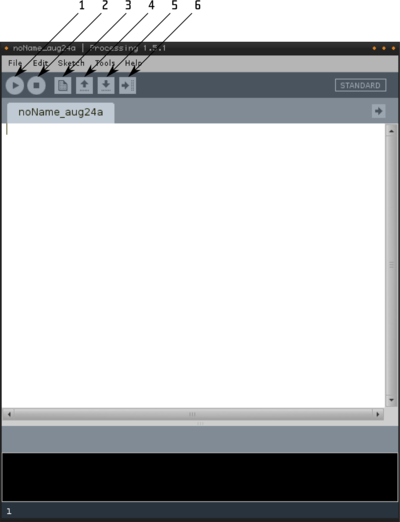
\includegraphics[width = 0.8\textwidth]{imgs/processing.png}
\end{center}


Základní rozhraní tvoří textový editor s několika nezbytnými funkcemi. Patrně nejdůležitější je v liště tlačítko {\em (1)} \klavesy{RUN}, které kompiluje a spouští program aktuálně rozpracovaný v textovém editoru. {\em (2)} Tlačítko \klavesy{STOP} naopak program zastaví. V případě chyby v programu je lze též využít jako vynucené zavření programu. Zbylá tlačítka slouží k diskovým operacím.\bublina{Zkuste nyní spustit Processing, bude dobré ho mít při ruce. Nemáte-li \nlb jej po ruce, doporučuji přeskočit následující kapitoly věnované prostředí.} \index{PDE}


\pododdil{Základní diskové operace}

Jsou to operace, jež něco zapisují či načítají z disku. Tyto operace zahrnují veškerou manipulaci se sketchí, její vytvoření, uložení, načtení či export do webového formátu či kompilaci do spustitelné aplikace.

Processingová sketch nemusí být nutně uložena, abyste ji mohli spustit. Nové úpravy, které v textovém poli napíšete, budou dočasně uloženy v závislosti na vašem operačním systému jinde. Tímto způsobem můžete experimentovat s kódem, aniž byste přišli o předchozí verzi.

Mezi základní operace patří vytvoření nové sketche {\em (3)}, otevření předešlé {\em (4)}, uložení {\em (5)} a export programu do webového appletu {\em (6)}.

Tlačítka mají dále speciální vlastnosti s podržením tlačítka: tlačítko s novou sketchí otevře také nové okno editoru. V kombinaci s načtením předchozí sketche {\em (4)} otevřete též sketch v novém editoru, aniž byste ztratili předchozí okno. U uložení se modifikace projevuje funkcí {\em uložit jako}. Při exportu přepínáte stisknutím klávesy \klavesy{SHIFT} mezi exportem samostatné aplikace nebo appletu\poznamka{Pouze ve verzi 1.x, {\em Processing 2.0} již export do appletu nepodporuje.}, aplikace schopné běžet v prohlížeči nebo obecně na webových stránkách. \index{ovládání}


\pododdil{Sketch}

Sketch je v {\em Processingu} označení pro jednotlivé projekty. Sketch je ve své podstatě složka obsahující alespoň jeden stejně nazvaný soubor s příponou {\em *.pde}. Sketch při vytvoření nevyžaduje název, je jí přidělen pouze aktuální datový kód zaznamenávající datum vytvoření. Tímto decentním způsobem {\em Processing} toleruje například nejasnost záměru autora při vytváření nového díla, jeho název či pracovní název lze tímto způsobem přiřadit až později, po nabytí jasnějších obrysů.

Program si vystačí pouze se samotným zdrojovým kódem, tj. souborem (soubory) {\em *.pde}. Ovšem operujeme-li s externími daty stojícími mimo zdrojový kód, můžeme využít dvě možnosti. Za prvé soubor, se kterým potřebujeme operovat, tažením myši přesunout na textové pole {\em Processing \index{PDE}PDE}. Touto operací bude soubor zapsán do naší sketche automaticky. Nebo lze operaci provést manuálně, stačí vytvořit v adresáři sketche adresář \lnb s názvem \slovnik{DATA}. {\em Processing} tuto složku automaticky rozpozná a soubory v této složce budou dobře dostupné pro pozdější operace.

Typy standardních adresářů, které se často objevují ve struktuře sketche, si stačí zapamatovat jen dva:

\begin{enumerate}
\item
adresář nazvaný {\em DATA} -- Tento adresář je využíván při práci s jakýmikoli vnějšími daty, jako jsou například obrázky, zvuky, videa, vektorové grafiky nebo textové soubory.

\item
adresář nazvaný {\em CODE}, obsahující externí zdrojový kód, případně kód kompilovaný v podobě knihovny mající nejčastěji přípony \lnb {\em *.java, *.class, *.jre}. -- Tento adresář se nalézá v systémové cestě daného projektu, a umístíme-li zde soubory, budou též dobře dostupné z daného projektu. (Adresář {\em CODE} nás zatím nemusí příliš zajímat, později se jeho prostřednictvím můžeme pokusit rozšiřovat funkce {\em Processingu} externím kódem.)

\end{enumerate}


\pododdil{Sketchbook}

Místo na disku, které {\em Processing} využívá k uskladnění sketchí, se nazývá povšechně {\em sketchbook} a je v podstatě pouze adresářem obsahujícím jednotlivé projekty. Koncepce {\em sketchbooku} spočívá v uspořádání jednotlivých projektů do organizované formy, a ačkoli nevnáší do jednotlivých projektů sám o sobě řád, může napomoci k vytvoření řádu vlastního. Ze své zkušenosti mohu říci, že organizace jednotlivých projektů do jakékoli struktury má opravdu smysl. Mnou preferovaná struktura obsahuje jednotlivé roky následně ještě dělené do měsíců, ale možnosti organizace záleží čistě na uživatelských preferencích. Tímto chci spíše ilustrovat možnost uspořádání nežli nezbytnost, ale přítomnost vašeho systému od počátku vřele doporučuji.

Ve {\em sketchbooku} se dále nachází jeden speciální adresář nazvaný {\em libraries}. Adresář v sobě uchovává externí rozšíření {\em Processingu} o komunitní knihovny. Standardně {\em Processing} již své základní knihovny nese v sobě, \lnb tj. jsou běžně přidány do samotného {\em Processingu}. V tomto adresáři se nacházejí knihovny, které budete moci použít později. Na stránkách projektu {\em http://processing.org} můžete nalézt velké množství komunitních knihoven s dobrou dokumentací volně ke stažení. Veškeré tyto knihovny tedy {\em Processing} potřebuje nalézt v tomto adresáři.






\pododdil{Editor}

Editor je textové pole a je vaším hlavním nástrojem komunikace s {\em Processingem}. Veškeré informace, které zadáte do tohoto pole, budou interpretovány samotným {\em Processingem}. Textový editor není nijak dokonalý, pro začátek si s ním ovšem vystačíme. Formát, který tento editor produkuje, je ve své podstatě textový soubor s příponou {\em *.pde}. \index{textový editor}




Textový editor má několik funkcí, které vám mohou usnadnit práci. \lnb Odlišuje například mezi příkazy {\em Processingu} barvami -- tato zdánlivá drobnost speciálně v začátcích napomůže, nebo v případě objemnějších kódů může výrazně zpřehlednit, organizaci programu. Jedná se o programátorskou konvenci obecně v anglickém jazyce nazývanou \slovnik{syntax highlighting}.


Další konvencí, se kterou se často setkáte, je tzv. \slovnik{indenting}, zarovnávání kódu do úhledných paragrafů. V {\em Processingu} si ze začátku vystačíte se standardním zarovnáním, posléze lze zarovnávání aktivovat stiskem kombinace kláves \klavesy{CONTROL (APPLE) + T}.


\begin{center}
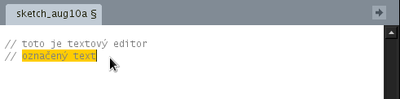
\includegraphics[width = 1\textwidth]{imgs/editor.png}
\end{center}

Horní lišta editoru označuje záložky, kliknutím na šipku na pravé straně lišty se vám zobrazí možnosti operací se záložkami. Pro začátek \lnb s nimi nebudeme pracovat. V případě delšího kódu záložky slouží k lepší organizaci struktury programu. V podstatě se dá říci, že každá záložka \lnb odpovídá jednomu souboru ve sketchi \odkaz{Sketch}.

Jak můžete vidět na obrázku, editor operuje i s českými znaky, ačkoli bych je z důvodů internacionalizace neradil používat. V komentářích, \lnb tj. textem uvozeným dvěma dopřednými lomítky \uv{//}, což je text, který kompiler ignoruje, jsou diakritická znaménka přípustná.

Naopak v případě názvu proměnných nebo jakýchkoli funkčních definic je použití diakritiky nepřípustné.\poznamka{Standardní jazykové kódování, ve kterém {\em Processing} operuje, je {\em UTF-8}.}


\oddil{Klávesové zkratky}

\begin{itemize}
\item[\klavesy{CTRL + r}]  spustí program
\item[\klavesy{CTRL + SHIFT + r}] takzvaný present mode spustí program a zatemní zbytek obrazovky
\item[\klavesy{CTRL + t}] automatické formátování textu, zarovnává text do odrážek
\item[\klavesy{CTRL + k}] otevře adresář konkrétního projektu
\item[\klavesy{CTRL + f}] vyhledávání v textu a nástroj pro hromadné nahrazování
\item[\klavesy{CTRL + SHIFT + f}] vyhledávání u označeného příkazu v referencích
\item[\klavesy{CTRL + s}] uloží projekt na disk
\item[\klavesy{CTRL + SHIFT + s}] uložit jako

\item[\klavesy{CTRL + e}] export jako webový applet\poznamka{Pouze v {\em Processingu 1.0}.}, otevře exportovaný projekt
\item[\klavesy{CTRL + SHIFT + e}] export jako aplikace, zobrazí okno s výběrem platforem pro export

\end{itemize}

* \klavesy{CTRL} značí klávesu \klavesy{CTRL} na PC a \klavesy{APPLE} na Mac



\oddil{Soustředěná činnost}

Než začneme doopravdy programovat, musíme si uvědomit, že tento proces vyžaduje velikou dávku koncentrace. Obecně se nedá říci, jaké fyzické prostředí je k programování ideální. To se samozřejmě může lišit. Ale platí, že fyzický prostor, který k programování potřebujete, je prostor, ve kterém se můžete sami soustředit na práci.

Koncentrace při psaní programu je specifická dovednost, kterou se začátečník učí jen stěží. Bohužel pouhým čtením této knihy se již vyvádíte \lnb z potenciální koncentrace. Učení se programovat je náročný proces a vyžaduje velikou dávku koncentrace sám o sobě. Okamžité zkoušení nových poznatků pomáhá zápisu informací do vaší dlouhodobé paměti a opakování je samozřejmě nezbytné k utužení těchto struktur. Co je, bohužel, při počátečním programování nezbytné, je například hledání v referencích a spolu se soustředěním se na program samotný je celý proces učení se velmi náročný na koncentraci.



V problematice programování obecně platí, že není nic složitějšího než číst cizí kód, nebo dokonce kód vlastní s odstupem času. Při programování se lidská mysl dostává do stavu mimořádné bdělosti a koncentrace. Tento stav je často popisován programátory jako tzv. \slovnik{flow}. Jedná se o stav, ve kterém mysl vědomě udržuje celý program\poznamka{Nebo větší části programu.} v paměti.

Pokaždé, když si programátor takový stav přivodí, vše v kódu\poznamka{Podle míry ovládnutí programovacího jazyka.} se pro něj jeví srozumitelné. Formátování a standardy velmi napomáhají k rychlému navození bdělého stavu, protože samy o sobě jsou jistou formou jazyka.

\oddil{Základní pravidla a zvyklosti}

V programování obecně platí jisté zákonitosti. Není tomu jinak ani u pravidel, která nejsou důležitá pro čtení kódu strojem, ale spíše pro člověka. Speciální zákonitosti formátování kódu mají ryze praktickou funkci. Jedná se o standard dodržovaný programátory, aby byli schopni sdílet své úsilí. \bublina{Otevřete některý \lnb z příkladů \lnb z lišty {\em File $\rightarrow$ Examples}, a letmo se seznamte s kódem. I když mu nebudete rozumět, podívejte se, jaká znaménka a barvy se v kódu opakují.}
  

\chapter{Stavba programu a~syntax}

  
\oddil{Logika programování}
Pro začátek je dobré si představit program jako sadu instrukcí. Každá \lnb instrukce má svůj význam a své místo. Instrukce se píšou v programovacím jazyku a jejich interpretace je vždy pro stroj jednoznačná. Stroje podle svého návrhu neudělají nic, kromě toho, co mají instruováno.

Veškeré programy, které používáte, dokonce i programy, o nichž nevíte, že používáte, byly někdy naprogramovány lidmi pomocí programovacích jazyků. Programovací jazyk je pouze plánovací forma zápisu programu. \lnb K tomu, aby byl program spuštěn, musí být v případě jazyka {\em Processing} převeden do strojového kódu. Strojový kód se liší od toho zdrojového, našeho čitelného plánovacího jazyka tím, že není čitelný pro člověka, je čitelný pro stroj.

Počítač je pouhý stroj. Umí opravdu rychle vykonávat sled banálních operací. Programovací jazyk slouží k vytvoření smyslu v těchto operacích. Proces převodu ze zdrojového kódu do strojového se nazývá kompilace.

O kompilaci toho nemusíme naštěstí mnoho vědět, vše bylo již tvůrci {\em Processingu} a jazyku {\em Java} shrnuto pod tlačítko \klavesy{RUN}.\bublina{Budete-li \nlb mít otevřený nějaký kód z~Examples, zkuste ho nyní spustit, uvidíte, jak se program chová. Vyzkoušejte několik příkladů.}


%\part{Stavba programu a syntax}



\pododdil{Komentář}
\label{komentar}

Komentář je vše, co program ignoruje. Je to místo v programu určené ke čtení člověkem. Komentáře dále často slouží k rychlé editaci programu. Odkomentováním řádky funkčního kódu lze vynechat některé funkce {\em Processingu}.


Následuje zápis tak, jak jej již můžete vepsat do editoru {\em Processingu}. Vřele doporučuji mít v této chvíli {\em Processing} čtení knihy zapnutý a po ruce, abyste si příklady v rámečcích mohli vyzkoušet. Komentář je řádek textu nebo jeho část uvozená dvěma dopřednými lomítky.


\begin{lstlisting}
// komentar je uvozen dvema doprednymi lomitky
\end{lstlisting}

Spustíte-li nyní program tlačítkem \klavesy{RUN}, objeví se šedé okénko prvního processingového programu. Jelikož jste zatím nedefinovali nic funkčního, program také nic nedělá. \index{komentáře v kódu}

V praxi je pak často využíván i druhý způsob komentáře, takzvaný víceřádkový komentář. Ten začíná dopředným lomítkem a hvězdičkou a~končí těmito znaky v obráceném pořadí.

\begin{lstlisting}
/* viceradkovy komentar je uvozen
doprednym lomitkem a hvezdickou
ukoncen hvezdickou a lomitkem 
(v obracenem poradi)

toto je viceradkovy KOMENTAR
toto je viceradkovy KOMENTAR
toto je viceradkovy KOMENTAR
toto je viceradkovy KOMENTAR
*/

/*zacatek .............. konec*/

\end{lstlisting}

Komentáře v {\em Processingu} poznáte vždy nejrychleji tak, že je bude editor obarvovat šedou barvou. \bublina{Vyzkoušejte si napsat nějaký text do textového editoru, spusťte program, následně před něj vložte dvě dopředná lomítka, pozorujte rozdíl.}

\pododdil{Základní datatypy}

K stavbě programu potřebujeme stavební materiál. Pro základní pochopení fungování programu je nezbytné nejdříve pochopit základní datatypy. Datatyp si lze obecně představit jako obálku na informaci.

{\em Processing} rozlišuje mezi jednotlivými datatypy. Informace, které se nacházejí v paměti, se musejí nacházet pod správným datatypem, aby program věděl, jak s nimi operovat.

K datatypu je možné si představit různé paralely, má oblíbená je podobnost s obálkami nebo nádobami. Různé datatypy si můžeme představit jako tvary nádob. Do rozličných nádob lišících se tvarem se směstná rozmanitý obsah. Typy obsahů se dají názorně představit na rozdílu mezi textovou informací a informací číselnou.

{\em Processing} potřebuje nejdříve vědět, zda nádoba obsahuje text, nebo číslo, aby s ní mohl operovat. Například nelze provést matematickou operaci mezi dvěma slovy. Sčítat, odčítat, dělit či násobit se dají pouze čísla.


\pododdil{Seznam základních datatypů}
\index{datatypy}
Datatypů je jen několik, dají se vcelku snadno zapamatovat:

\begin{lstlisting}
int mojeCeleCislo = 1;

float mojeCisloSDesetinnouCarkou = 1.33;

boolean mojePravdaCiNepravda = true;

String mujSlovniRetezec = "Ahoj svete!";

char mujJednotlivyZnak = 'A';

\end{lstlisting}

Takovému zápisu již bude {\em Processing} rozumět. Vepsáním těchto řádků do processingového editoru již dochází k alokaci vašich informací ve správných datatypech v paměti. Vysvětleme si nyní několik nejasností.

První slovo na každém řádku označuje odlišný datatyp (náš tvar nádoby), následuje jméno proměnné (název pro naši nádobu), poté může následovat rovnítko, které již přiřazuje obsah -- hodnotu do proměnné (nádoba je naplněna).

Každý příkaz je ukončen středníkem \uv{;}.

Podivné názvy takzvaných proměnných, jako například {\em mojeCeleCislo}, jen ukazují, že název pro svoji proměnnou můžete zvolit téměř podle libosti. Proměnná ale nesmí mít v názvu mezeru, tedy prázdný znak. Podle zvyklostí by dále proměnná měla začínat malým písmenem, a potřebuje-\lnb te-li nutně použít víceslovný název, napište velké písmeno místo mezery.

Proměnná nesmí být číslo, ale slovní název. Programátorské konvence při pojmenovávání proměnných jsou ryze praktické. Proměnná by měla mít co možná nejkratší a nejvýstižnější název.  Toto je spíše dobré doporučení nežli pravidlo. Správným pojmenováním proměnných docílíte větší přehlednosti v kódu, kratší délkou si ušetříte zbytečné psaní. \bublina{Bedlivě si prostudujte jednotlivé datatypy, přepište je do Processingu a~zkuste pojmenovat po~svém. Podle toho, co mohou reprezentovat, přiřaďte patřičné hodnoty.}


\pododdil{Barva}

Zvláštním datatypem v {\em Processingu} je datatyp určený pro barvy, \vyraz{color()}. Barvy lze definovat následujícími způsoby. 

\begin{lstlisting}
// skala sede, 0 = cerna, 255 = bila
color mojeBarvaSeda = color(127);

// skala sede s pruhlednosti
color mojeBarvaSeda2 = color(255,127);

// cervena, modra, zelena
color mojeBarvaOranzova = color(255,127,0);
   
// cervena, modra, zelena, pruhlednost 
color mojeBarvaOranzova2 = color(255,127,0,127);
   
// barva vyjadrena stylem HTML, v hexadecimalnim tvaru
color mojeBarvaOranzova3 = color(#FFCC00);
\end{lstlisting}

Pro výběr oblíbené barvy lze využít nástroj z lišty {\em Tools $\rightarrow$ Color \lnb Selector}.

Základní barevné nastavení je 24bitové RGB, to znamená, že každá barevná hloubka jednoho kanálu je 8 bitů, což značí 256 možných stupňů. Nejvyšší stupeň je ovšem 255, jelikož ten nejnižší není 1, nýbrž 0.

Kolorimetrické prostory a jejich rozmezí se dají volně definovat pomocí příkazu \vyraz{colorMode()}.\bublina{Otevřete si lištu Tools $\rightarrow$ Color Selector, zkuste vybrat několik barev a přepsat je do správného tvaru.}


\pododdil{Tisk do konzole}
\index{konzole}
Tento jednoduchý program zatím jen definoval několik proměnných do správných datových typů a nedělá nic zajímavého. Celá alokace probíhá uvnitř programu. {\em Processing} provádí většinu svých operací skrytě. Program kreslí nebo jinak interaguje s uživatelem, jen je-li o to požádán.

Nejjednodušší výstup z programu je tisk do tzv. konzole. Konzoli jsme si již krátce uvedli v kapitole {\em Základní prostředí}. V {\em Processingu} se konzole nachází pod textovým editorem. Toto černé pole má pouze textový výstup a slouží k doladění programu.

Tiskem do konzole si nyní můžeme například zkontrolovat obsah našich proměnných. To můžeme provést následujícími dvěma způsoby:


\begin{lstlisting}
print(mojeCeleCislo);

println(mujSlovniRetezec);
\end{lstlisting}

Oba příkazy tisknou obsah našich proměnných. Jediný rozdíl mezi příkazy je ten, že druhý příkaz končí znakem:
 
\begin{lstlisting}
"\n"
\end{lstlisting}

Jedná se o tzv. {\em newline character}, přidáním speciálního charakteru příkaz tiskne pokaždé na nový řádek. Není nutné si pamatovat tento speciální znak, postačí, když si zapamatujeme příkaz 

\begin{lstlisting}
println( cokoli );

\end{lstlisting}

Spustíme-li program nyní, v konzoli se nám ukáže výstup z našeho programu:

\console{1Ahoj svete!}\\

Zde je názorně vidět, že tisk pomocí pouhého příkazu \vyraz{print()} nepoložil další příkaz na nový řádek, a tedy vytiskl {\em 1Ahoj} dohromady.

Tisk do konzole se hojně používá při ladění programu. Kdykoli se na něco potřebujete kódu zeptat, můžete tak učinit tímto prostým příkazem.

V konzoli se tisk projevuje bílou barvou. Další možný obsah konzole jsou chyby. Ty jsou označeny barvou červenou. {\em Processing} vám chybou naznačuje, že něco není v pořádku s vaším kódem. V případě takto jednoduchého programu se v drtivé většině případů bude jednat o překlep či zapomenutý znak.

Programovací jazyk, bohužel (naštěstí?), neodpouští překlepy. Tedy bude stačit jeden chybný znak v programu, aby celý program nebyl spustitelný.

Bohužel chybové hlášení se nedá označit za dokonalé a pro začátečníky bude velmi složité dobrat se pomocí chybových hlášení původu chyby. Na zlepšení chybových hlášek se pracuje již dlouhou dobu a některé základní chyby {\em Processing} v angličtině umí dobře popsat. Většinou ale {\em Processing} tiskne řetězec svých chyb, které byly nastartovány chybou vaší, a chybová hlášení čítající několik desítek řádků vám toho nakonec o původní chybě moc nesdělí.

V případě chyby se vás {\em Processing} bude snažit přesměrovat na řádek, kde chyba pravděpodobně vznikla. V případě takto jednoduchých programů, jaké si zde ukazujeme, chybu identifikuje zcela bezchybně, bohužel tomu tak nebude ve všech případech.\bublina{Vyzkoušejte si vytisknout různé proměnné, ověřte, zdali tisknou hodnoty, které jste jim zadali.}\index{chybové hlášení}


\pododdil{Základní operace s datatypy}

Náš program nyní neprovádí nic světoborného. Definuje několik proměn\-ných a následně některé z nich tiskne do konzole. Operujeme zde stále s~\uv{abstraktními} hodnotami, které se zapisují do paměti programu a pak je z paměti zpětně získáváme.

Nyní si ukážeme, co s již definovanými proměnnými můžeme dělat. Jednotlivé datatypy mají různé přípustné operace. Zkusme si letmo projít možnosti našich proměnných.

\begin{itemize}


\item{{\em Integer} a {\em float} neboli čísla: {\em int} a {\em float}}

První proměnná {\em mojeCeleCislo}, které byla přiřazena hodnota {\em 1}, je takzvaný {\em Integer}, tedy celé číslo. Tento typ může mít hodnotu\poznamka{Na 32bitových strojích.} v~rozsahu -$2147483648$ až $2147483647$. V rozmezí těchto hodnot můžeme provádět různé matematické operace s čísly:

\begin{lstlisting}
int prvniCislo = 1;
int druheCislo = 5;
int tretiCislo;

tretiCislo = prvniCislo + druheCislo;

println(tretiCislo);
\end{lstlisting}

Tímto jsme provedli základní matematickou operaci, sečetli jsme dvě čísla a následně jsme výsledek vytiskli do konzole.

\pagebreak

Další možné operace jsou:

\begin{lstlisting}
// aritmeticke operace
a + b;
a - b;
a * b;
a / b;

// prirustky
a += b;
a -= b;

// prirustek, ubytek o 1
a ++;
a --;

// modulo (prebytek po deleni)
a % b;

// a porovnavani
// vetsi, mensi
a < b;
a > b;

//vetsi nebo rovna se, mensi nebo rovna se
a <= b;
a >= b;

// shoda, neshoda
a == b;
a != b;

// pozor, vysledkem porovnavani jiz neni cislo
// ale odpoved ANO, nebo NE, TRUE, nebo FALSE
// pravda, nebo nepravda, datatyp boolean

\end{lstlisting}

S celými čísly neboli {\em int} nebude problém se sčítáním, odčítáním \lnb a násobením. V případě dělení může nastat logicky problém, výsledek nemusí být celé číslo. Budeme-li chtít výsledek takové operace uchovat v paměti, tj. zapsat pod naši proměnnou, musíme použít datatyp operující s desetinnou čárkou nebo výsledek zaokrouhlit.

\pagebreak
Například:

\begin{lstlisting}
int a = 10;
int b = 3;
float c;

c = a / b;

println(c); 
\end{lstlisting}

Vytiskne:

\console{3}

Pozor, to není správný výsledek! Kde se stala chyba? {\em Processing} operující s celými čísly speciálně při dělení předpokládá výsledek opět celé číslo. Tedy ono zaokrouhlení provádí již sám. Stačí si nyní pamatovat, že pro přesné dělení čísel bychom měli dělit vždy číslem s desetinnou čárkou, tj. s datatypem {\em float}.

Tedy správně by dělení mělo proběhnout takto:

\begin{lstlisting}
float a = 10;
float b = 3;
float c;

c = a / b;

println(c); 
\end{lstlisting}

Tisk do konzole již ukazuje \uv{správnou} hodnotu:

\console{3.333333}

Pro další operace s čísly bych pro přesnost výsledků důrazně doporučil používat jen {\em float}. Další operace mohou vypadat například takto:

\begin{lstlisting}
float a = 3;
float b;

// sq je funkce pro "square", cislo na druhou
b = sq(a);
println(b);

// sqrt je funkce pro "square root", odmocninu
b = sqrt(a);
println(b);

// pow je funkce pro "power", cislo na N-tou
// minusova cisla v N jsou odmocniny
b = pow(a,3);
println(b);

b = pow(a,-3);
println(b);

// atp.
\end{lstlisting}

\item{{\em char} a {\em String}}, znak a řetězec znaků, text}

S textem nelze operovat stejně jako s čísly, je logické, že nemůžeme násobit texty mezi sebou. {\em String} je speciální datatyp pro uchovávání textů v paměti a nakládá se s ním speciálními funkcemi. Prozatím nám bude stačit, když si ukážeme velmi jednoduchou operaci s textem, spojení dvou řetězců dohromady.
\index{práce s textem}

Pro označení hodnoty řetězce se používají dvojité uvozovky. S textem se pracuje následovně:

\begin{lstlisting}
String prvniSlovo = "Ahoj";
String druheSlovo = "svete!";
String slovniSpojeni;

slovniSpojeni = prvniSlovo + " " + druheSlovo;

println("Dve spojena slova: " + slovniSpojeni);
\end{lstlisting}

Všimněte si, prosím, mezery vložené mezi slova. Uvozená mezera je také řetězec textu. Výsledným tiskem do konzole tedy dostaneme následující řetězec textu:

\console{Dve spojena slova: Ahoj svete!}


Zde jsme provedli jednu ze základních operací s textem, spojování řetězců. {\em String} lze také spojit s jednotlivými znaky nebo i s čísly, výsledkem bude ovšem vždy další {\em String}.

\begin{lstlisting}
int a = 1;
int b = 2;
String slova = "test";

// "slova = slova + neco" lze take nahradit znamenkem "+="
// stejnym znamenkem, ktere u cisel znamena prirustek,
// tedy namisto:
// slova = slova + " " + a + " " + b;
// muzeme zkratit na:

slova += " " + a + " " + b;

println(slova);
\end{lstlisting}

Výsledkem bude: 

\console{test 1 2}\bublina{Pospojujte vlastní větu z~jednotlivých slov, vyzkoušejte do věty spojit i~čísla.}

Řetězce se dají dále porovnávat, seřazovat, lze v nich vyhledávat znak či slovo a tak podobně. Pro naše účely zatím postačí si uvědomit rozdílné operace mezi textem a číslem.


\item{{\em boolean} neboli pravda nebo nepravda}
\index{boolean}

{\em Boolean} je nejjednodušším datatypem v {\em Processingu}, může vyjadřovat pouze dva stavy. Pravdu {\em (true)} nebo nepravdu {\em (false)}. Žádnou jinou hodnotu {\em boolean} nepřijímá, a proto je, co se týče paměti, velmi úsporným datatypem. Operace s {\em booleany} se nazývají logické operace a vypadají následovně:


\begin{lstlisting}
boolean prvniTvrzeni = true;
boolean druheTvrzeni = false;
boolean tretiTvrzeni;

// "&&" znaci logickou operaci AND
// vysledek bude TRUE, pravda, JEN pokud
// prvniTvrzeni a druheTvrzeni bude pravda
tretiTvrzeni = prvniTvrzeni && druheTvrzeni;

println(tretiTvrzeni);

// "||" dve svisle cary je OR, tj "nebo"
// vysledek bude TRUE, pravda, pokud
// prvniTvrzeni nebo druheTvrzeni je pravda
tretiTvrzeni = prvniTvrzeni || druheTvrzeni;

println(tretiTvrzeni);

// posledni zakladni operaci je porovnani
// muzeme porovnat dva booleany pomoci "=="
// dvojiteho rovnitka
tretiTvrzeni = (prvniTvrzeni == druheTvrzeni);

println(tretiTvrzeni);

// pro negativni vysledek je zaporne porovnani "!="
// vykricnik pred booleanem vzdy znaci opak

tretiTvrzeni = (prvniTvrzeni != druheTvrzeni);

println(tretiTvrzeni);

\end{lstlisting}

{\em Boolean} je možné si představit jako vypínač světla. Zapnuto a vypnuto jsou jediné dva stavy podobného vypínače. {\em Booleany} často řídí tok programu, je možné si je představit jako přepínače mezi jednotlivými stavy programu.

\end{itemize}


\pododdil{Základní struktura programu}
\index{funkce setup() a draw()}
{\em Processing} rozlišuje mezi jednotlivými programovacími přístupy. Textový editor se automaticky přizpůsobí způsobu programování. Tímto přístupem se {\em Processing} snaží co nejvíce přiblížit začátečníkovi. Základní prostředí nám dovoluje pouze nakreslit tvary a ukončit program. K pohybu v čase musíme {\em Processingu} definovat základní strukturu programu.

Dvě nejzákladnější funkce, se kterými se budeme při programování \lnb setkávat, jsou \vyraz{setup()} a \vyraz{draw()}:

\begin{itemize}
\item
\vyraz{setup()} je funkcí, která bude spuštěna jednou, na začátku programu \lnb -- zde se nejčastěji nastavují počáteční parametry, které si potřebujeme připravit, než se spustí kreslicí funkce

\item
\vyraz{draw()} je funkce pro opakované kreslení, bude spouštěna stále po dobu chodu programu -- tady budeme nejčastěji kreslit tvary a provádět proměnlivé výpočty pro animaci
\end{itemize} 


Základní funkce pro vyvolání překreslování výstupního okna je funkce \vyraz{draw()}. Funkce je uvozena slovem \vyraz{void}. O funkcích se více dozvíme později \odkaz{Funkce}. Jedná se o základní smyčku, která zajišťuje jakoukoli proměnlivost, tedy animaci v obraze. Smyčka je de facto operace, která v programu vyjadřuje rozměr času.

Základní struktura bude vypadat asi takto:


\begin{lstlisting}
void setup(){ 
  
  size(200,200);
  frameRate(15); 
  println("tisk z funkce setup()");  

}


void draw(){

  background(0); 
  println("tisk z funkce draw() " + frameCount);  

}

\end{lstlisting}

Po spuštění programu uvidíte v konzoli následující výstup:


\begin{lstlisting}
tisk z funkce setup()
tisk z funkce draw() 1
tisk z funkce draw() 2
tisk z funkce draw() 3
tisk z funkce draw() 4

\end{lstlisting}
\bublina{Velmi pozorně si pročtěte předchozí dva příklady. Ujistěte se, zda rozumíte dobře rozdílu mezi setup() a~draw(), pro další pokračování bude pochopení klíčové.}

\oddil{Zobrazení}

\pododdil{Orientace v prostoru}
\index{prostor}
Okno programu by se dalo přirovnat k listu papíru, popřípadě k malířskému plátnu. Ve standardním dvoudimenzionálním modu má dva základní parametry, $X$ a $Y$, označující souřadnice, ve kterých se veškeré kreslicí operace pohybují. Důležité je zmínit, že oproti jisté konvenci v matematických grafech nese levý horní roh hodnotu $X = 0$, $Y = 0$. Směrem dolů hodnota $Y$ přibývá, stejně tak jako hodnota $X$ přibývá směrem doprava:

\begin{center}
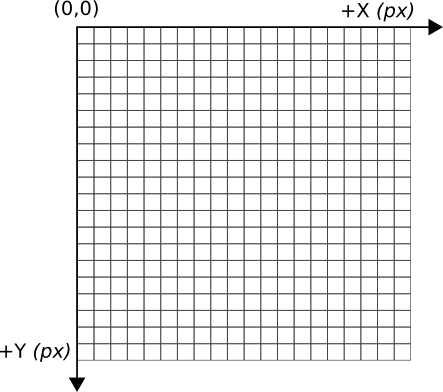
\includegraphics[width = 0.65\textwidth]{imgs/grid2d.png}
\end{center}

Tato konvence je převzata ze standardu počítačové grafiky, kdy první pixel v levém horním rohu nese souřadnicovou hodnotu právě $X = 0$, $Y = 0$. Obrácená osa $Y$ se může ze začátku jevit matoucí. Důvody pro zdánlivé převrácení os pochopíme později, například právě při operacích se samotnými obrazovými body, pixely, které jsou standardně uspořádány od levého horního rohu doprava a níže.

Plochu je možné si představit jako prázdný prostor, na kterém lze zobrazovat grafiku. Tvary nebo kupříkladu text se zobrazují právě prostřednictvím zdrojového kódu, tj. instrukcemi psanými v editoru.

Na první pohled by se mohlo zdát, že je kód například při zobrazení obdélníka příkazem:

\begin{lstlisting}
rect(x,y,sirka,vyska);
\end{lstlisting}

jehož výsledkem je kresba pouhého obdélníka, zbytečně komplikovaný oproti jiným zobrazovacím metodám. Důležité je si zde uvědomit koncepci {\em Processingu}, který tímto zobrazením primitivních objektů sestavuje celý obraz. To, co se zpočátku může zdát jako nadbytečná práce, tedy psaní \lnb koordinátů každého ze zobrazovaných objektů, se posléze ukáže jako sofistikovaný a velmi ulehčující způsob přemýšlení o obraze. Veškeré parametry oddělené čárkou v kulatých závorkách příkazu {\em rect} náleží samotným vstupním hodnotám. Příkaz {\em rect} očekává čtyři parametry. Parametry mohou být celá čísla nebo čísla s desetinnou čárkou. Pro názornost, zadáme-li do parametrů \uv{natvrdo} hodnoty:

\begin{lstlisting}
rect(8,6,7,5);
\end{lstlisting}

výsledné zobrazení na naší pomyslné ploše bude zhruba následující:

\begin{center}
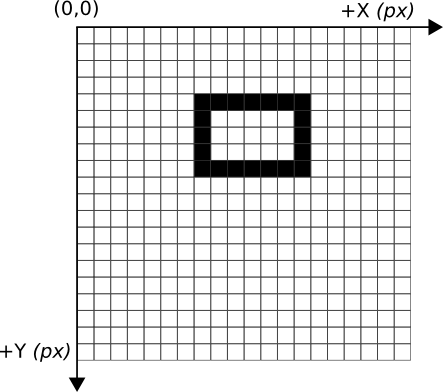
\includegraphics[width = 0.65\textwidth]{imgs/gridRect2d.png}
\end{center}


Zamyslíme-li se kupříkladu nad tím, že bychom v jakémkoli jiném nástroji chtěli zobrazit vícero, například tisíc obdélníků, na první pohled jednodušší GUI \poznamka{Zkratka pro Guided User Interface klasické grafické editory jako Gimp nebo Photoshop.} grafické editory nám nedovolí tuto operaci učinit jinak, než že musíme všech tisíc obdélníků nakreslit. V případě {\em Processingu} nám bude stačit vytvořit rutinu pro kreslení libovolného počtu obdélníků a pak tuto rutinu spustit.

Zde se již dostáváme k samotnému jádru processingového přemýšlení. Programování obecně dokáže velmi ulehčit operace, jejichž pravidelnost dovedeme popsat. Veškeré umění psaní programu tedy spočívá v definicích těchto chování a redukci složitých jevů na jednoduché rovnice.

Celé řemeslné umění psaní kódu v podstatě záleží na eleganci zápisu složitějších vztahů mezi různými parametry. Dovednosti se člověk učí postupně, osvojení si gramatické korektnosti a logické posloupnosti se mohou zpočátku jevit zbytečně komplikované, ovšem už po ovládnutí pouhých pár jednoduchých pravidel lze {\em Processing} využít kreativním způsobem. \bublina{Zkuste si na kus papíru, nejlépe čtverečkovaného, nakreslit jednotlivé objekty. Uvědomte si, v jakých dimenzích se pohybují.}


\oddil{Hodnota a její zobrazení}

K čemu jsou vlastně hodnoty dobré? Tisk do konzole je jen kontrolní mechanismus, většinou se nejedná o výslednou podobu programu.

Po celou dobu sčítání a odčítání hodnot jsme nevyvolali žádnou funkci, která by kreslila na plátno.

Nyní je na čase ukázat si, jakým způsobem {\em Processing} rozumí kresbě. Tytéž hodnoty, které máme nyní v paměti, mohou být použity pro jakýkoli kreslený výstup. Řekněme, že chceme z těchto hodnot zobrazit například elipsu. K tomu potřebujeme vyvolat funkci pro tvorbu elipsy, pokud ji nechceme zrovna z nějakých důvodů popisovat matematicky (to je samozřejmě dobře možné).

{\em Processing} nemá předdefinované žádné složité tvary. Pracuje sám o~sobě pouze s tvary primitivními, jako je bod, linka, trojúhelník, obdélník a~elipsa. Pomocí těchto tvarů lze zkonstruovat nepřeberné množství obrazů. Před\-stavíme-li si nyní digitálně zpracovanou fotografii, můžeme kupříkladu říci, že je zkonstruována z bodů. Jednotlivé body, tj. pixely, mají jinou barevnou hodnotu a takto poskládaný obraz se ve výsledku jeví jako fotografie.

Problém v případě konstrukce syntetické fotografie nespočívá v geomet\-rii; to je známá mřížka bodů s počtem šířky krát výšky obrazových bodů digitální fotografie. Problém je v barevných hodnotách, které neznáme a~synteticky je jakoukoli matematickou funkcí velmi těžko obsáhneme.

Dat pro výpočet fotorealistického obrazu potřebujeme opravdu hodně, nástroje, které dokážou simulovat fotorealistický obraz, existují a není jich málo. Dokonce i v {\em Processingu} existují podobná rozšíření, která přímo zpracovávají a zajišťují obrazový výstup.

Tento příklad je trochu extrémní, ale naprosto pravdivý. Věc, kterou se snažím ilustrovat, je, že i s minimálním počtem primitivních geometrických tvarů lze docílit téměř nekonečného (spočitatelně obrovského) množství obrazů, což by nám mělo dlouho stačit.

Nyní zpět k hodnotám. Máme-li již jakékoli hodnoty v paměti programu, můžeme kterékoli z nich použít na jakoukoli kreslicí funkci. Zde začíná naše experimentální část, často se totiž stává, že výsledek kreslení neumíme plně předpovědět a teprve zobrazením nám kresba vzhledem k~hodnotě začne dávat smysl.

\oddil{Kresba}

Jak zobrazit hodnoty, které uchovává program v paměti? Jakoukoli hodnotu lze použít například jako jeden z vstupů (tzv. argumentů) v kreslicích funkcích.

Již zmiňovaný \vyraz{rect()}, tedy rectangle -- obdélník, vyžaduje k svému úspěšnému vykreslení čtyři parametry, čtyři číselné hodnoty\poznamka{Zde nezáleží, jestli se jedná o celé číslo {\em (int)} nebo číslo s desetinnou čárkou {\em (float)}.}. Tyto parametry, hodnoty, můžeme buď zadat jako přímé číselné hodnoty, nebo do těchto parametrů můžeme zadat naši proměnnou, která obsahuje číslo.

Názorně:

\begin{lstlisting}

// prvni zpusob vykresleni obdeniku
rect(10, 8, 40, 20);

// druhy zpusob vykresleni obdelniku
int prvniCislo = 10;
int druheCislo = 8;

rect(prvniCislo, druheCislo, 40, 20);

\end{lstlisting}


\begin{center}
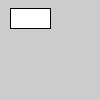
\includegraphics[width = 0.2\textwidth]{imgs/kresba-1.png}
\end{center}

Nyní je nám zřejmé, jak hodnoty mohou ovlivnit zobrazení. Místo hodnot zadaných číselně se zde v druhém způsobu vykreslení obdélníku objevují naše proměnné, které již mají zadaný obsah. Výsledek zobrazení bude v obou případech stejný, ovšem z hlediska struktury programu je druhý způsob daleko flexibilnější.
\index{tvary 2D}

V {\em Processingu} je předdefinovaných jen několik základních tvarů, se kterými lze bohatě vystačit. Kromě již zmíněného \vyraz{rect()} jsou zde také základní tvary:

\begin{itemize}
\item[\vyraz{point()}] bod ($X$, $Y$)
\item[\vyraz{line()}] čára ($X_1$, $Y_1$, $X_2$, $Y_2$)
\item[\vyraz{ellipse()}] elipsa ($X$, $Y$, šířka, výška)
\item[\vyraz{triangle()}] trojúhelník ($X_1$, $Y_1$, $X_2$, $Y_2$, $X_3$, $Y_3$)
\item[\vyraz{quad()}] čtyřúhelník ($X_1$, $Y_1$, $X_2$, $Y_2$, $X_3$, $Y_3$, $X_4$, $Y_4$) 

\end{itemize}\bublina{Nakreslete jeden bod, čáru a~elipsu tak, aby se vzájemně nepřekrývaly. Zkuste změnit jejich pořadí, sledujte změny po spuštění.}

\pododdil{Výplň a obrys}

Některé tvary mají výplň a jiné (\vyraz{point()} a \vyraz{line()}) pouze konturu. Potřebuje-me-li změnit barvu kresby objektů, můžeme použít vědomosti z předchozí kapitoly \odkaz{Barva}.

Výplň je definována jednou barevnou hodnotou přidanou do funkce \vyraz{fill()}. V kódu bude zápis vypadat následovně:

\begin{lstlisting}
fill(255,127,0);
rect(10, 10, 40, 20);

fill(0,127,255);
rect(10, 40, 40, 20);

\end{lstlisting}


\begin{center}
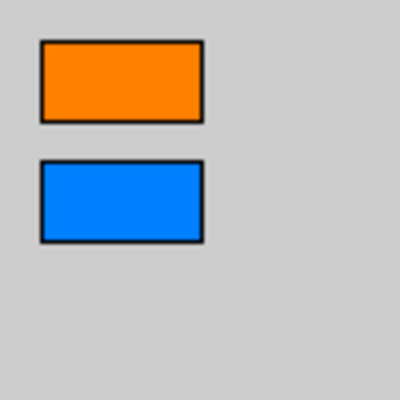
\includegraphics[width = 0.2\textwidth]{imgs/vypln-1.png}
\end{center}

Opak příkazu \vyraz{fill()} je \vyraz{noFill()}. Potřebujeme-li vykreslovat u objektů s~výplní pouze jejich konturu, můžeme použít právě příkaz \vyraz{noFill()}.

K ovládání barvy kontury použijeme příkaz \vyraz{stroke()}, ten opět přijímá hodnotu barvy. Jeho opakem je \vyraz{noStroke()}.

Ukažme si názorně zápisy:

\begin{lstlisting}
fill(255, 127, 0);
noStroke();
rect(10, 10, 40, 20);

noFill();
stroke(0,127,255);
rect(10, 40, 40, 20);

noFill();
stroke(0,127,255);
triangle(80, 70, 60, 60, 90, 30);


stroke(255);
line(10, 80, 90, 90);

\end{lstlisting}

Všimněte si zde pořadí, v jakém příkazy určují výsledný obraz. Jeden příkaz na změnu barvy bude aplikován postupně na všechny objekty, které poté budou vykresleny, dokud opět nezměníte nastavení barev pro kresbu.

Výsledek kódu vypadá následovně:

\begin{center}

\includegraphics[width = 0.2\textwidth]{imgs/vypln-2.png}
\end{center}




Představme si nyní, že hodnota zadaná prvním způsobem zápisu se již nikdy v průběhu programu nemůže proměnit. V případě druhého způsobu zápisu získáváme díky možnosti změny jednoho parametru kontrolu nad kresebným výstupem.

Veškeré příkazy, které jsme si zatím ukázali, byly spuštěny pouze jednou. To znamená, že obdélník byl vykreslen a program, který již neměl žádné další příkazy, jednoduše skončil.

V další kapitole si předvedeme, jak vdechnout procesům pohyb a stálost, následující kapitola je věnována animaci.



\oddil{Pohyb}

\pododdil{Proměnlivost}


Potřebujeme-li programu vdechnout život, musíme nejprve pochopit, jakým způsobem se program může proměňovat.

Proměnlivost se dotýká základní myšlenky programu trvajícího v čase. K tomu, abychom takovou proměnlivost mohli okem pozorovat, program může komunikovat pomocí různých výstupů. {\em Processing}, který byl navržen s důrazem na vizuální výstup, bude nejčastěji komunikovat právě obrazem. Obecně řečeno, proměnlivost je jakákoli změna hodnot v délce běhu programu, lze si ji představit například jako rozdíl mezi dvěma okénky filmu.

U filmových okének je rozdíl sice velmi těžko definovatelný, ilustruje ovšem dobře celý problém. Film nám zprostředkovává iluzi pohybu sledem několika okének za vteřinu. Stejně se chová i vizuální program. Rozdíl mezi filmem a programem je zhruba ten, že program může mít teoreticky dva a více různých konců, nebo nemusí končit vůbec. Zde by se dalo namítnout, že program je také nakonec nositelem kauzálního sledu operací. Vtip je v tom, že stejný program spuštěný dvakrát nemusí produkovat stejný výsledek.

Změny v chodu programu se dá docílit několika způsoby. Základní změna v běhu programu je lidská intervence, která je z pohledu programu, respektive tvůrce programu, jen velmi těžko předpovídatelná. Změna v chování programu bez takového vnějšího zásahu je pak vždy umělá \odkaz{Náhoda}.


Vraťme se ovšem k proměnlivosti. Proměnlivost je nezbytnou součástí animace. Pohyb je proměna stavu v čase. Měli bychom mít vždy na paměti, že program nerozumí tomu, co zrovna zobrazuje, program rozumí pouze hodnotám. Rozpohybovat lze tyto hodnoty, a tím posléze například jevy, které se v programu zobrazují a člověku dávají nějaký smysl. 

Pro příklad si můžeme ukázat, jak proměna jedné hodnoty ovlivňuje \lnb obraz. K tomu, abychom mohli hodnotu proměňovat, ji musíme nejdříve pojmenovat.

\begin{lstlisting}
int y = 0;
\end{lstlisting}

Tímto jsme pojmenovali svoji proměnnou. Jednou z možných variant zápisu je okamžité přiřazení hodnoty, tedy {\em y} je nyní nula. Pro animaci hodnoty použijeme přírůstek, tedy při kresbě jednotlivého okénka přičteme k~hodnotě $1$. Abychom viděli nějaký výsledek, můžeme opět kreslit objekt, který bude využívat proměňující se hodnotu v čase.

\begin{lstlisting}
void setup(){
	size(640,480);
}

void draw(){
	background(255);
	
	// prirustek o jedna
	// lze zapsat i zkracene y++;
	y += 1;
	
	// kresba
	line(0 ,y ,width ,y);

}
\end{lstlisting}

Po spuštění tohoto programu uvidíte animaci trvající $480$ okének. Animace bude pokračovat i nadále, hodnota {\em y} se bude stále proměňovat. Kresba bude teoreticky probíhat mimo plátno. K tomu, abychom kresbu udrželi v~mezích plátna, můžeme použít jednoduchou podmínku, která bude vracet hodnotu {\em y} zpět na nulu.


\begin{lstlisting}
if(y > height){
	y = 0;
}
\end{lstlisting}

Celá tato procedura jen ilustruje logiku programu. Hodnota {\em y} je zde přímo zobrazena, ale stejně tak se dá použít kdekoli jinde, tedy ne nezbytně na kresbu. Pro lepší představu jiného použití uvedu následující příklad.

Pod hodnotou si lze například představit pevně stanovenou hodnotu, dejme tomu výšku domu. Zadání výšky nepostaví dům, ale stanoví hodnotu, se kterou můžeme dál počítat. Známe-li výšku plánované budovy, můžeme kupříkladu přidávat patra, dokud se této výšky nedosáhne. Tuto proceduru již lze považovat za logickou konstrukci a jedním ze základních postupů, jak takové logiky v programu docílit, je podmínka \odkaz{Podmínka}. \bublina{Vyzkoušejte přidat podmínku na konec programu nebo ji vynechat, ujistěte se, že rozumíte tomu, co v animaci způsobuje, zaměňte číslo v~podmínce za jiné, s nižší hodnotou a~pozorujte výsledek.}

\pododdil{Animace}

Statická kresba na plátno je jen jeden z možných výstupů. Animace v {\em Processingu} znamená, jak jsme si ukázali v předchozím příkladě, překreslovat plátno pokaždé jinými obrazy. Nyní si ukážeme základní pojetí tvorby \lnb pohyblivého obrazu.

Jak jsme si již uvedli dříve \odkaz{Základní struktura programu} funkce \vyraz{draw()} je pouze prostředek pro změnu, nepřináší změnu sama o~sobě. Funkce \vyraz{draw()} zajišťuje sousledné vyvolání příkazů v neustálém  trvání\poznamka{Po dobu běhu programu.}. V {\em Processingu} si v podstatě uvědomíme, že psaním příkazů do smyčky píšeme pravidla jakoby pro jedno okénko filmu. Pohyb je vždy zajištěn proměnou našich datatypů \odkaz{Základní datatypy}, které v~tomto okénku figurují.

Tedy například napíšeme-li takto samotnou smyčku:

\begin{lstlisting}
void draw(){
	// 60x za vterinu spustena operace
}
\end{lstlisting}

vše uzavřené do složených závorek bude spuštěno šedesátkrát za vteřinu. Bude-li obsah základní funkce \vyraz{draw()} neměnný, tj. budeme-li vyvolávat šedesátkrát za vteřinu totéž, animace tím bude v případě vizuálního výstupu jen abstraktním pojmem.

V tomto příkladu již dochází k spuštění smyčky. Výsledkem bude pouze šedivá plocha o rozměrech sto krát sto pixelů, jelikož na plátno nebylo zatím nic vykresleno. Následujícími příkazy \vyraz{background()} a \vyraz{rect()} nakreslíme nejprve plné pozadí a následně obdélník.

\pagebreak
Zápis bude vypadat takto:

\begin{lstlisting}
void draw(){
	background(255);
	rect(10 , 10 , 30 , 30);
}
\end{lstlisting}

Takový zápis již provádí animaci a kreslí na plátno. Animace ovšem v~tomto případě nebude patrná, jelikož zatím se v obraze nic neproměňuje. Veškeré hodnoty jsou statické, tudíž se vykresluje jeden čtverec na bílém pozadí na stále stejném místě.

K rozhýbání objektů jednoduše potřebujeme proměnit jeden z~paramet\-rů v čase. \bublina{Animace je proměna obrazu v čase, jednotlivá okénka se v čase musí lišit. Přemýšlejte, jakým způsobem k~proměně může dojít.}  Abychom docílili animace, zkusme například vložit místo parametru pro kresbu čtverce v ose $X$ počitadlo okének. {\em Processing} má již nastavenou proměnnou s údajem o počtu uběhlých okének pod názvem \vyraz{frameCount}.

Proměnnou \vyraz{frameCount} lze využít následovně:

\begin{lstlisting}
void setup(){
	size(640,480);
}

void draw(){
	background(255);
	rect( frameCount % width , 10 , 30 , 30 );
}

\end{lstlisting}

Výsledkem tohoto zápisu bude opět animace. Čtverec se bude pohybovat rychlostí šedesáti pixelů za vteřinu zleva doprava. Tato hodnota v~podstatě udává počet vykreslených cyklů funkce \vyraz{draw()}, ta je v tomto případě pouze využita k pohybu vykreslovaného čtverce.

Počet okének vykreslovaných za vteřinu můžeme ovlivnit pomocí \lnb funkce \vyraz{frameRate()} vložené do funkce \vyraz{setup()}.

Tento pohyb je velmi názorný, ukazuje, že hodnotu počtu vykreslených okének lze použít například i jako hodnotu pro animaci. Stejně tak si můžeme založit i vlastní proměnnou, která bude mít identickou funkci.\poznamka{V tomto konkrétním příkladu to sice nedává smysl, dá se použít stejně tak standardní proměnná \vyraz{frameCount}, ukázka je zde jen pro ilustraci možností využití proměnných.}

\pagebreak

\begin{lstlisting}
// nase promenna nazvana priznacne: pocitadlo
int pocitadlo = 0;


void setup(){
	size(640,480);
	frameRate(30);
}

void draw(){
	background(0);
	rect( pocitadlo, 10 , 30 , 30 );

	// zde jiz pricitame hodnotu, lze napsat i zkracenym zapisem:
	// pocitadlo++;

	pocitadlo += 1;

	// zde muzeme pouzit modulo na omezeni pocitadla na sirku platna

	pocitadlo = pocitadlo % width;

}

\end{lstlisting}

Definicí této hodnoty lze například časovat animace. Další metodou je animaci časovat pomocí funkce \vyraz{millis()}. Tato funkce je nezávislá na počtu vykreslených okének za vteřinu, měří počet uběhnutých milisekund od startu programu. Může se nám také hodit pro precizní časování událostí v~programu.


\pododdil{Dynamika pohybu}

K docílení jednoduché interakce není zapotřebí mnoho. Animace je ovšem složitější problém, který budeme řešit v {\em Processingu} nejvíce matematicky. Zdá se, že dosažení dynamického pohybu je jeden z průvodních jevů pokročilého programování.

\pagebreak

 Nyní si můžeme ukázat, jak lze zkombinovat dosavadní znalosti k vytvoření nelineárního pohybu:
 
 \begin{lstlisting}
float x;
float y;
float rychlost;

void setup(){
	size(640,480);
     x = width / 2;
     y = height / 2;
     rychlost = 0.1;
}

void draw(){
	background(255);
	x += (mouseX - x) * rychlost;
	y += (mouseY - y) * rychlost;
	rect(x,y,30,30);
}
\end{lstlisting}

Čtverec bude nyní následovat kurzor nelineárním pohybem. Dynamika pohybu je dána prostou formulí:
\begin{lstlisting}
x += (mouseX - x) * rychlost;
y += (mouseY - y) * rychlost; 
\end{lstlisting}\bublina{Opište formuli a zkuste změnit rychlost, pozorujte změny, pozměníte hodnoty tak, aby se objekt pohyboval po křivce.}
K proměnným {\em x} a {\em y} přiřazujeme zlomek rozdílu mezi pozicí kurzoru a proměnnou v obou osách. Tuto formuli lze využít téměř kdekoli, například při jemném přechodu barev a vyhlazování hodnot obecně.

Druhá proměnná, {\em rychlost}, by se k docílení podobného efektu měla pohybovat v rozmezí od $0$ do $1$.
\index{nelineární pohyb}



\oddil{Podmínka}

Po seznámení s proměnlivostí procesů se můžeme dostat k prvnímu opravdovému strukturování programu. Zkusme nyní nastínit, jak taková struktura vypadá. Patrně nejpřímější řízení dějů v programu je podmínka. Podmínka říká: Jestliže je něco pravda, spusť následné příkazy. Podmínka funguje v podstatě jako výhybka, která odklání program do jeho různých cest. Uvedu zde krátký příklad vytváření podobné struktury v programu:

\begin{lstlisting}
boolean prepinac = false;
int hodnota;

if(prepinac == true){
    hodnota = 1;
}else{
    hodnota = 0;
}

println(hodnota);

\end{lstlisting}

Velmi prostá struktura je v tomto příkladu vytvořena jednou podmínkou. Podmínka je v {\em Processingu} (a řadě jiných jazyků) značena slovem \vyraz{if}, \uv{jestli}. \uv{Jestli} potřebuje dostat odpověď na otázku v kulatých závorkách (ta může být jen pravda nebo nepravda), k tomu se hodí nejlépe již zmíněný \vyraz{boolean}. Výsledkem {\em booleanu} může být porovnávání dvou čísel, znaků nebo řetězců znaků, tj. operace, které nám vrátí \vyraz{true} nebo \vyraz{false}.

Definujeme-li tedy náš \vyraz{boolean} na začátku jako nepravdu, podmínka se v tomto případě nenaplní a program spustí kód uvozený složenými závorkami následujícími až slovo \vyraz{else}.

V našem příkladu se jedná o druhou větev podmínky; ta sice není povinná, ale pro ukázku jsem ji zde rovnou zmínil. Tedy za ukončením \vyraz{if} a~vložením složených závorek můžeme dále za slovem \vyraz{else}, \uv{jestliže ne}, říci, co se stane v případě nenaplnění naší podmínky.

V tomto konkrétním případě se k proměnné {\em hodnota} přiřadí číslo $0$.

To program následně ověřuje tiskem do konzole, kde se objeví $0$.


\pododdil{If}

Jak jsme si již uvedli, podmínka je jedním ze základních stavebních kamenů programu. Podmínku lze použít ve všech případech, kdy předpokládáme jednoznačnou odpověď {\em ano} nebo {\em ne}. Podmínka v {\em Processingu}, stejně jako v řadě ostatních jazyků, je vytvořena příkazem \vyraz{if}.


\pagebreak
Konstrukce podmínky vypadá pak následovně:


\begin{lstlisting}

boolean pravda = true;

if(pravda == true){

    // spust nasledujici blok

}

\end{lstlisting}

Za povšimnutí zde stojí dvojité rovnítko. Tento speciální symbol se po\-užívá při již zmíněném porovnávání dvou stran. Proměnná nazvaná {\em pravda} získala hodnotu \vyraz{true}. V případě podmínky nezáleží na počtu proměnných v kulatých závorkách, otázka může být i více kombinována. Záleží na výsledku, který vždy musí být pravda nebo nepravda, tedy \vyraz{true} anebo \vyraz{false}. Pro zkonstruování takové věty lze použít následující znaménka: \bublina{Vyzkoušejte i jiné logické operace, ujistěte se, že správně rozumíte, jak fungují, použijte vykřičník jako zápor, změňte logické operace.}

\begin{lstlisting}
boolean pravda = true;
int cislo = 3;
String text = "Lorem ipsum dolor et amet";

if(cislo == 3){
    // tato podminka je spustena
}

if(cislo != 3){
    // tato podminka neni spustena, znamenko nerovna se je opakem rovnitka
}

if(cislo > 3){
    // tato podminka neni spustena, cislo neni vetsi nez 3
}

if(cislo < 3){
    // tato podminka neni spustena, cislo neni mensi nez 3
}

if(cislo >= 3){
    // tato podminka je spustena, znamenko vetsi nebo rovna se, cislo rovna se 3
}

if(cislo <= 3){
    // tato podminka je spustena, znamenko mensi nebo rovna se, cislo rovna se 3
}

if(text.equals("Lorem ipsum dolor et amet")){
	// tato podminka je spustena, porovnavani textu je take mozne, ovsem pozor
	// k porovnavani celych retezcu textu se pouziva funkce equals("String")
}

\end{lstlisting}

Takovým výčtem operací jsme si pokryli základní konstrukci podmínky. Další znaménka slouží k skládání jednotlivých otázek. Znaménko pro logické \uv{A} je \uv{\&\&}. Používá se následovně:

\begin{lstlisting}
boolean a = true;
boolean b = false;

if(a == true && b == false){
	// tento blok bude spusten, a je pravda A b je pravda
}

if(a == true && b == true){
	// tento blok nebude spusten, b totiz neni pravda, b == false
}

\end{lstlisting}


\uv{Ampersand} se na české klávesnici nevyskytuje, na anglické klávesnici jej naleznete většinou pod \klavesy {SHIFT - 7}, pro logické \uv{nebo} se používá dvojitá svislá čára \uv{||}, tzv. pipe:

\begin{lstlisting}
boolean a = true;
boolean b = false;

if(a == true || b == false){

	// tento blok bude spusten, k tomu staci pouze, ze a je pravda NEBO b je pravda

}


if(a == true || b == true){

	// tento blok bude tedy opet spusten

}


if(a == false || b == true){

	// tento blok jiz spusten nebude, a ani b neni pravda 

}

\end{lstlisting}

Pomocí skládání otázek můžeme zkonstruovat celé věty a složitější podmínky. V kombinaci s~kulatými závorkami si vystačíme pouze s~logickým {\em AND} a~{\em OR}. Pokusme se ilustrovat situaci následovně:


\begin{lstlisting}
boolean a = true;
boolean b = true;
boolean c = false;

if( (a && b) || c ){

	// tento blok bude spusten
	
}

if( !(a && b) || c ){

	// tento blok nebude spusten
	
}

\end{lstlisting}

Jaký je rozdíl mezi prvním a druhým blokem? Poslední specialita booleanovských operací je znaménko vykřičník. Takové znaménko před proměnnou typu \vyraz{boolean} znamená opak tvrzení, tedy, je-li {\em pravda} pravdou, {\em !pravda} \label{!pravda} je nepravdou, výsledkem je \vyraz{false}.\bublina{Zkuste si v duchu představit otázky, na které lze odpovědět \uv{ano} nebo \uv{ne}, zkuste je poté přepsat do tvaru podmínky, zkuste k~tomu využít další proměnné, porovnávejte je a~pokuste se přemýšlet, k~čemu se dají takto využít.}


\begin{lstlisting}
boolean pravda = true;

println( pravda ); // tiskne true
println( !pravda ); // tiskne false
\end{lstlisting}



Dále si všimněte, že v podmínce chybí jakékoli porovnávací znaménko. Ve skutečném programování se setkáte spíše s tímto zápisem, je to zápis zkrácený. Místo neustálého rozepisování {\em něco rovná se rovná se \vyraz{true}} lze napsat pouze v kulatých závorkách. Je-li naše {\em něco} datového typu \vyraz{boolean}, {\em Processing} bude takovému zápisu rozumět. Tedy nejjednodušší zápis může vypadat i takto:

  
\begin{lstlisting}
boolean a = true;

if(a)
	;//pouze tento jediny radek bude spusten
	
	
if(a){
	// cely tento blok
	// bude spusten
}
\end{lstlisting}

K úplnému zkrácení se dají vypustit i složené závorky, to vede opět k~rychlejšímu zápisu. Rozdílem takového zápisu je fakt, že taková podmínka spouští pouze jeden následující řádek. Přestože je to naprosto správný způsob programování, někteří programátoři takový zápis neradi používají kvůli zhoršení přehlednosti v kódu. Opět se s takovým zápisem často setkáte, člověk je jednoduše líný živočišný druh a \vyraz{if} se v programování po\-užívá opravdu často.

\pododdil{Else}

K dalšímu rozšíření podmínek slouží již zmíněný příkaz \vyraz{else} a dá se přeložit takto: jestliže je něco pravda, udělej toto, jestliže ne, proveď něco jiného. Zápis vypadá následovně:

\begin{lstlisting}
boolean a = false;

if(a){

	// kdyby a bylo true, tak by se spustil tento blok kodu 

}else{

	// ale protoze je nase a false, spusti se nyni kod
	// v tomto bloku
	
}
\end{lstlisting}



\pododdil{ ? : }

Abychom podmínky vyčerpali nadobro, ukážeme si poslední možný zápis, který může být ještě úspornější. \bublina{Vyzkoušejte si zkrácené zápisy, ověřujte jejich funkčnost tiskem do konzole nebo například proměnou barev objektů.}
  
  
\begin{lstlisting}
boolean a = true;

if(a)
background(0);
	
	
background( a ? 0 : 255 );

\end{lstlisting}






\oddil{Interakce}

\Slovnik{interakce} se dá obecně definovat jako vzájemné působení. V počítačové terminologii se má nejčastěji na mysli vzájemné působení člověka a stroje. Přímá interakce, která znamená vzájemné působení dvou prvků, předpokládá rozměr času\poznamka{Tedy program trvající v čase.}. Takový rozměr trvání programu v čase umožňuje uživateli přímý vstup do proměnných, tedy do obsahu našich hodnot.

Je dobré si uvědomit, že \slovnik{interakce} je do jisté míry při práci s počítačem pozorovatelná neustále. Pouhý pohyb myši lze považovat za interakci člověka se strojem. Pohyb uživatele přímo proměňuje hodnoty vykreslující pozici kurzoru, stiskem klávesy v textovém editoru píšeme text atp.

Při interakci je nutné do určité míry předvídat chování uživatele. Interakce primárně vychází z fyzické zkušenosti s předměty kolem nás, je jí myšleno vše, co může uživatel přímo ovlivnit.

Interakce se dá rozdělit do dvou základních oblastí -- na interakci přímou a nepřímou nebo, chcete-li, na interakci vědomou a nevědomou. Mezi těmito kategoriemi neexistuje jednoznačná hranice.

Obecně je toto rozlišení spíše stupnicí od jednoduchých, přímo a okamžitě viditelných jevů po uživatelově vstupu ke komplikovanějším procedurám spouštěným jen s částečným (nebo žádným) vědomím uživatele.

\pagebreak

Základní, tedy přímou interakci si můžeme ukázat v následujícím příkladu:

\begin{lstlisting}
void setup(){
	size(640,480);
}

void draw(){
	background(0);
	// vsimnete si parametru mouseX a mouseY
	rect(mouseX,mouseY,30,30);
}
\end{lstlisting}


\begin{center}
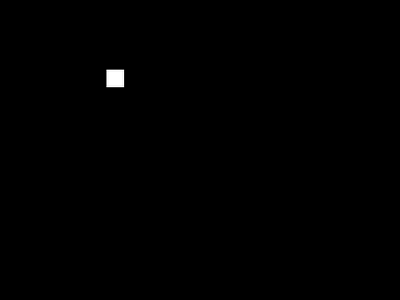
\includegraphics[width = 0.8\textwidth]{imgs/interakce-1.png}
\end{center}

Toto je jedna z nejzákladnějších možných interakcí. Vstupem pro pozici kresleného obdélníka se nám stávají dva parametry \vyraz{mouseX} a \vyraz{mouseY}.

Čtení pozice myši je jedním z nejsnazších možných způsobů interakce stroje s člověkem. Nyní si ukážeme, jak lze detekovat stisknutí tlačítka myši. Pro tento účel můžeme využít předdefinovaných metod {\em Processingu}. K detekci kliku lze použít funkci \vyraz{mousePressed()}.

\pagebreak

\begin{lstlisting}
boolean stisknuto = false;

void setup(){
	size(640,480);
}

void draw(){
	background(0);
	
	if(stisknuto){
		fill(255);
	}else{
		fill(255,0,0);
	}
	
	rect(mouseX,mouseY,30,30);
}

void mousePressed(){
	stisknuto = !stisknuto;
}

\end{lstlisting}


\begin{center}
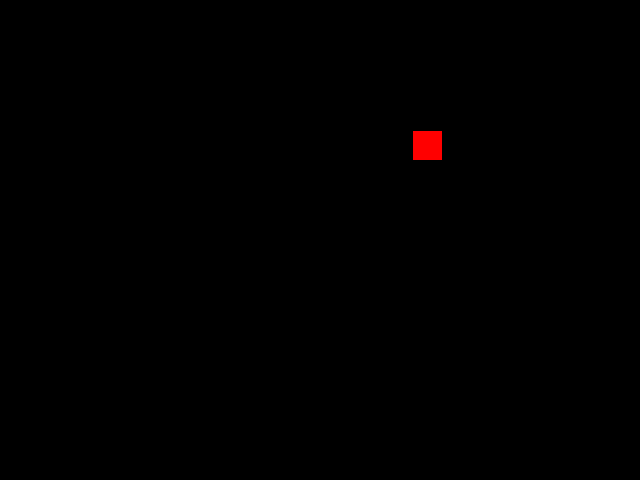
\includegraphics[width = 0.8\textwidth]{imgs/interakce-2.png}
\end{center}

Všimněte si poslední funkce \odkaz{Funkce}. Ta je programem spuštěna jen tehdy, stiskne-li uživatel tlačítko myši. Abychom uchovali in\-formaci o stisku, přepneme jím stav jedné z~našich proměnných nazvané {\em stisknuto}. Jednořádkový zápis s vykřičníkem je zkrácení pro přepnutí stavu \odkaz{Podmínka}.

K tomu, abychom detekovali stisk tlačítka myši, použijeme funkci \vyraz{mousePressed()}. Další možností interakce je detekovat, které tlačítko myši jsme stiskli, popřípadě detekovat stisk klávesy. Výčet dalších možností je následující:


\begin{lstlisting}
// detekce stisku tri ruznych tlacitek mysi
void mousePressed(){
	if(mouseButton==LEFT){
	
	}else if(mouseButton==RIGHT){
	
	}else if(mouseButton==CENTER){
	
	}
}


// detekce tazeni stisknute mysi
void mouseDragged(){
	// muzeme zde opet detekovat tlacitko
}

// timto detekujeme moment
// uvolneni stisku tlacitka
void mouseReleased(){
	// opet zde muzeme detekovat, ktere
	// tlacitko bylo stisknuto
}

// stisk klavesy s detekci typu
void keyPressed(){

	if(key=='a'){
	
	}else if(keyCode=='ENTER'){
	
	}
}


// detekce uvolneni klavesy
void keyReleased(){

}

\end{lstlisting}

Tímto výčtem jsme v podstatě vyčerpali možnosti interakce se standardními vstupy uživatele v {\em Processingu}. Veškeré tyto definice musí stát mimo základní funkce {\em Processingu}, tedy mimo \vyraz{setup()} a \vyraz{draw()}.

Proměnná \vyraz{mouseButton} nám říká údaj o naposledy stisknutém tlačítku myši, stejně tak funguje proměnná \vyraz{key} a \vyraz{keyCode} ve funkci \vyraz{keyPressed()} a~\vyraz{keyReleased()}.

Obě proměnné \vyraz{key} a \vyraz{keyCode} jsou buď vyjádřeny číslem, které lze vyhledat například v mapě znaků, nebo znakem ve tvaru {\em char}. Hodnotu \vyraz{key} lze také porovnávat přímo se znakem uvozeným apostrofy (například {\em 'k'}). V případě \vyraz{keyCode} lze porovnávat hodnotu kódovaných kláves.

Jestli je klávesa kódovaná, zjistíme dále pomocí proměnné \vyraz{CODED}. Asi takto:

\begin{lstlisting}
void keyPressed(){

	if(key == CODED){
		if(keyCode==ENTER){
			// detekce klavesy ENTER
		}
	}else{
		if(key==' '){
			// detekce mezerniku
			// porovnano s prazdnym znakem
		}
	}
}
\end{lstlisting}

Hrubý výčet pojmenovaných kláves, které můžeme porovnat s proměnnou \vyraz{keyCode}, je následující:

\begin{lstlisting}
// spiky
UP, DOWN, LEFT, RIGHT

// specialni klavesy
ALT, CONTROL, SHIFT

// dalsi dulezite klavesy
BACKSPACE, TAB, ENTER, RETURN, ESC, DELETE
\end{lstlisting}

Nevíme-li si rady, jak určitou klávesu detekovat, můžeme si jednoduše vytisknout do konzole její číslo pomocí  příkazu \vyraz{println()}.


\begin{lstlisting}
void keyPressed(){
	println("cislo klavesy: "+key);
}
\end{lstlisting}

\bublina{Vyzkoušejte detekovat různé klávesy, zkonstruujte jednoduché přepínače, které mohou \lnb reagovat na podněty.}


\oddil{Pole}

Jedna proměnná může uchovat pouze jednu hodnotu. V programování se brzy dostaneme do situace, kdy budeme potřebovat operovat s vícero hodnotami najednou. Tak například, chceme-li použít deset čísel z Fibonacciho řady, můžeme si je definovat postupně.

\begin{lstlisting}
int hodnota0 = 2;
int hodnota1 = 3;
int hodnota2 = 5;
int hodnota3 = 8;
int hodnota4 = 13;
int hodnota5 = 21;
int hodnota6 = 33;
int hodnota7 = 54;
int hodnota8 = 87;
int hodnota9 = 141;
\end{lstlisting}


K zkrácení zápisu místo neustálého přepisování téhož je zde takzvané pole. Pole neboli {\em Array} se v programování vyznačuje hranatými závorkami.

\begin{lstlisting}
int mojePoleHodnot[];
\end{lstlisting}

Všimněte si zde pouze hranatých závorek na konci názvu proměnné. Druhý možný zápis s naprosto identickým významem je vložit hranaté závorky před název definované proměnné.


\begin{lstlisting}
int [] mojePoleHodnot;
\end{lstlisting}

Oba způsoby jsou naprosto identické. Pouhá definice pole ovšem pole nevytváří. K tomu, abychom nyní do pole něco mohli začít ukládat, ho musíme nejprve inicializovat na pevný počet hodnot. V tomto případě lze hodnoty zadat přímo v definici pole. Pro takovou operaci je možné využít zápis pomocí složených závorek:

\begin{lstlisting}
int mojePoleHodnot[] = {0,1,1,2,3,5,8,13,21,33};
\end{lstlisting}

Tento zápis inicializace je v tomto konkrétním případě zřejmě nejrychlejší. Hodnoty z pole, které je nyní celé uloženo pod jednou proměnnou, můžeme získat následujícím způsobem:

\begin{lstlisting}
int mojePoleHodnot[] = {0,1,1,2,3,5,8,13,21,33};

println(mojePoleHodnot[0]);
println(mojePoleHodnot[1]);
println(mojePoleHodnot[5]);
//atd.
\end{lstlisting}


Další způsob zápisu je ovšem obvyklejší, a jak se dozvíme v příští kapitole \odkaz{Smyčka}, bude pro nás nejvýhodnější.


\begin{lstlisting}
int mojePoleHodnot[];

void setup(){
	mojePoleHodnot = new int[10];
	
	mojePoleHodnot[0] = 0;
	mojePoleHodnot[1] = 1;
	mojePoleHodnot[9] = 33;
	// atp.
}
\end{lstlisting}

Všimněte si, že  se v zápisu objevilo slovo \vyraz{new}. Toto slovo jsme zatím nepoužili a jeho význam rozvedeme později \odkaz{Třída a objekt}. \lnb K~tomu, abychom přiřadili hodnotu jednotlivých míst v poli, musíme nejdří\-ve uvést do hranatých závorek, kam budeme hodnotu zapisovat. Stejně tak se později k číslu, které jsme uložili, můžeme dostat. 

Tímto způsobem jsme si definovali pole o rozměru deseti hodnot. Stále je ovšem patrné, že v kódu se zbytečně opakujeme rozepisováním názvu jedné proměnné.\bublina{Pole jsou abstraktní koncepce. Ujistěte se, že dobře rozumíte, jakým způsobem pracují. Najděte si pro pole vhodnou paralelu, například číslované zásuvky pro představu fungují dobře, pročtěte si kapitolu klidně vícekrát, abyste polím dobře rozuměli.}

Hodnot v polích nebude vždy jen deset. K lepší práci s poli potřebujeme rychlejší způsob. Jak na to, zjistíte v následující kapitole věnované smyčkám. 


\oddil{Smyčka}


Smyčka je mocný nástroj a dobrý pomocník při práci s opakovanými operacemi. V minulé kapitole jsme si definovali pole. Definici nyní zopakujeme a zkusíme ji více automatizovat pomocí smyčky.


\begin{lstlisting}
int mojePoleHodnot[];

void setup(){
	mojePoleHodnot = new int[10];
	
	for(int i = 0; i < 10; i += 1){
		mojePoleHodnot[i] = 0;
	}
}
\end{lstlisting}

A první smyčka je na světě. Zápis, který na první pohled vypadá trochu odpudivě, může být váš dobrý přítel. Trochu si jej rozebereme. 

Formule začíná slovem \vyraz{for}. Následují kulaté závorky. V nich je v podstatě rozsah, který potřebujeme zopakovat. Hodnoty jsou odděleny středníkem. \bublina{Vyzkoušejte si rozdílné smyčky s~různým rozsahem, opakujte si složitější zápis \uv{for}, dokud jej nebudete umět sami bezchybně zkonstruovat, zkuste smyčku využít s~měnící se proměnnou uvnitř, kreslete ze smyčky objekt.}

\begin{itemize}
\item[počátek] int i = 0
\item[konec] i < 10
\item[přírůstek] i += 1
\end{itemize}

Hodnota, se kterou pracujeme, se jmenuje {\em i}, ale může se jmenovat dle vaší libosti například:

\begin{lstlisting}
	for(int pocitadlo = 0; pocitadlo < 10; pocitadlo += 1){
		mojePoleHodnot[pocitadlo] = 0;
	}
\end{lstlisting}

Podle potřeby lze také definovat rozsah smyčky. Kupříkladu počítání v~opačném pořadí:


\begin{lstlisting}
	for(int pocitadlo = 9; pocitadlo >= 0; pocitadlo -= 1){
		mojePoleHodnot[pocitadlo] = 0;
	}
\end{lstlisting}

Název pro jednoduchou smyčku {\em i} se používá velmi často, může například značit slovo {\em index}. Smyčky vykonávají v programu tvrdou práci, využívají se pro hromadné operace, z nichž se často stávají náročné výpočty.

Vraťme se ovšem k definici Fibonacciho řady z předchozí kapitoly \odkaz{Pole}. Pokusíme se nyní skloubit to, co jsme se naučili o smyčkách a polích. Zkusíme si napsat jednoduchý program, který nám vygeneruje tolik čísel z Fibonacciho řady, kolik budeme potřebovat.


\begin{lstlisting}
int delka = 18;
int fibonacci[];

void setup(){
	fibonacci = new int[delka];
	fibonacci[0] = 0;
	fibonacci[1] = 1;
	
	
	for(int i = 2; i < delka; i += 1){
		fibonacci[i] = fibonacci[i-1] + fibonacci[i-2];
	}
	
	println(fibonacci);
}

\end{lstlisting}

V konzoli se nám objeví:

\begin{lstlisting}
[0] 0
[1] 1
[2] 1
[3] 2
[4] 3
[5] 5
[6] 8
[7] 13
[8] 21
[9] 34
[10] 55
[11] 89
[12] 144
[13] 233
[14] 377
[15] 610
[16] 987
[17] 1597
\end{lstlisting}

Čísel samozřejmě může být nepočitatelně. Smyčky mají tu výhodu, že dokážou opakovat jednu operaci. Můžeme využít jazyka k definici operace a zapojením dalších proměnných ji povýšit na princip. Máme-li takto zpracovaný princip, můžeme jej například zobrazit nebo s ním dále pracovat. K lepšímu uspořádání se dostaneme v další kapitole \odkaz{Funkce}.

Pro ilustraci Fibonacciho řady můžeme využít druhou smyčku ke kresbě:

\begin{lstlisting}
for(int i = 0; i < delka; i += 1){
	line(fibonacci[i],0,fibonacci[i],height);
}
\end{lstlisting}

a výsledkem kresby bude:

\begin{center}

\includegraphics[width = 0.8\textwidth]{imgs/smycka-1.png}
\end{center}


\oddil{Uspořádání struktury programu}
\index{void}

Jednotlivé bloky kódu lze dále strukturovat. Strukturování v kódu se provádí zpravidla tam, kde potřebujeme opakovaně spouštět identický blok kódu nebo si zpřehlednit probíhající operace.


\pododdil{Funkce}

Nejjednodušším řešením problému je jeho rozdělení na menší části. Problém, jak dojít k jednomu výsledku, se dá rozložit na jednotlivé po sobě jdoucí události a ty postupně popsat.

Dílčí operace si pro přehlednost můžeme definovat do bloku takzvané funkce. Základní funkcí je \vyraz{void}. {\em Void} v podstatě tvoří blok kódu, který uceluje nějakou proceduru, ta může být posléze jednoduše spuštěna jedním příkazem. Jestliže by mohly jednotlivé proměnné ve větě označovat podstatná jména, funkce se dají například chápat jako slovesa. S funkcemi jsme se setkali již dříve při definici základních smyček programu.

\begin{lstlisting}

void setup(){

}

void draw(){
	nakresliObdelnik();
}

void nakresliObdelnik(){
	rect(10,10,20,20);
}

\end{lstlisting}

Vedle standardních funkcí {\em Processingu} \vyraz{setup()} a \vyraz{draw()} jsme si nyní definovali třetí funkci, nazvanou {\em nakresliObdelnik()}. Tato funkce je pak spuštěna uvnitř kreslicí smyčky \vyraz{draw()}.

V tomto konkrétním případě samotná funkce nedává mnoho smyslu. Příkaz \vyraz{rect()} v podstatě není nic jiného nežli funkce {\em Processingu} \uv{nakresli obdélník}. Všimněme si ovšem, že tato funkce \vyraz{rect()} má v kulatých závorkách parametry, které označují, kde má být obdélník vykreslen a jaké má mít rozměry. Tyto parametry se v programování obecně nazývají {\em arguments} nebo také vstupní hodnoty funkce.

Chceme-li vytvořit funkci a potřebujeme-li do ní poslat vstupní paramet\-ry, musíme při její definici vepsat do kulatých závorek, jaké paramet\-ry bude funkce očekávat.


\begin{lstlisting}

void nakresliObdelnik(int x, int y){
	rect( x , y , 20 , 20 );
}

\end{lstlisting}

Jednotlivé parametry se v kulatých závorkách oddělují čárkou a může jich být teoreticky neomezené množství. Parametry vždy musí dodržovat dané datatypy, v opačném případě {\em Processing} funkci nedokáže najít.

Důležité je upozornit, že vstupní hodnoty jsou vytvořeny pokaždé, \lnb spustíme-li funkci, a zanikají, je-li funkce ukončena. Takovým proměnným se říká dočasné nebo lokální. V programátorské praxi se můžeme setkat s~jejich uvozováním podtržítkem.

\pagebreak


\begin{lstlisting}

void nakresliObdelnik( int _x, int _y ){
	rect( _x , _y , 20 , 20 );
}

\end{lstlisting}

Podtržítka nemají žádný faktický význam, jsou jen součástí názvu proměnné a programátoři je používají pro lepší organizaci.

V {\em Processingu} lze dále definovat funkce, které se jmenují stejně, ty pak ale musí mít jinou skladbu vstupních hodnot. Představme si, že budeme potřebovat dvě funkce {\em nakresliObdelnik()}, jednu můžeme nechat bez vstupních parametrů a druhou budeme definovat parametry {\em x} a {\em y}. Tak můžeme odlišit dvě různé funkce pouze způsobem spuštění.

\begin{lstlisting}

void nakresliObdelnik( int _x, int _y ){
	rect( _x , _y , 20 , 20 );
}

void nakresliObdelnik(){
	rect( 10 , 10 , 20 , 20 );
}

void draw(){
	nakresliObdelnik();
	nakresliObdelnik( 10 , 20 );
}

\end{lstlisting}

Tento příklad je správně a vykreslí dva různé obdélníky. Máme nyní na výběr, potřebujeme-li zadat parametry, nebo ne, v druhém případě se nakreslí obdélník v předem nadefinované pozici.


{\em Void} je pouze jedna z možností definic funkcí. Další možné funkce můžeme definovat podle datatypů, které budeme očekávat jako výsledek funk\-ce. Tedy můžeme si definovat funkci, která nám zjistí, zdali se kurzor nachází v daném obdélníku. Místo prázdné funkce \vyraz{void} budeme očekávat odpověď ve tvaru \vyraz{boolean} pravda nebo nepravda. Funkce uvozená datatypem bude vždy očekávat odpověď ve stejném tvaru takového datatypu. Pomocí slova \vyraz{return} můžeme funkci přiřknout výsledek, v tomto případě \vyraz{true} nebo \vyraz{false}.

\pagebreak

\begin{lstlisting}

Void setup(){

	size(640,480);

}

void draw(){
	if( jeKurzorVObdelniku(10,20,20,20) ){
		nakresliObdelnik(10,20);
	}

}

boolean jeKurzorVObdelniku(int _x, int _y, int _sirka, int _vyska){
	
	if(mouseX >= _x && mouseX <= _x +_sirka &&
	mouseY >= _y && mouseY <= _y +_vyska){
	
		return true;
	
	}else{
	
		return false;
	
	}
}

void nakresliObdelnik(){
	rect( 10 , 10 , 20 , 20 );
}

void nakresliObdelnik(int _x, int _y){
	rect( _x , _y , 20 , 20 );
}

void nakresliObdelnik(int _x, int _y, int _sirka, int _vyska){
	rect( _x , _y , _sirka, _vyska );
}


\end{lstlisting}


Bude-li se kurzor nacházet v prostoru vymezeném v otázce, nakreslí se obdélník o stejné velikosti. Náš program již začíná být strukturovaný. Tímto způsobem můžeme dále větvit podmínky a rozdělovat kód do jednotlivých spustitelných bloků příkazů.

Funkce stejně jako proměnné doporučuji pojmenovávat stručně a výstižně. U funkcí dále platí, že by měly dělat pouze jednu věc a měly by ji provádět dobře. Je lepší problém rozdělit na více funkcí, a tím  strukturovat program. Strukturování podobným způsobem je velmi výhodné, budete-li se ke kódu vracet s odstupem času nebo bude-li jej číst někdo jiný než vy.

Budete-li kód chtít sdílet, je dobré jej učinit co nejvíce čitelným pro ostatní. Zde je velmi dobrá tradice napsat ke každé funkci jeden řádek nebo odstavec komentáře o tom, co funkce přesně dělá  (pokud to není na první pohled zřejmé).

Co se délky funkcí týče, dobré pravidlo zní: Přesáhne-li počet vnitřních proměnných tucet, měli byste už přemýšlet o rozdělení do dvou funkcí.

\pododdil{Funkce a jejich datatypy}

Funkce \vyraz{void} je jen jednou možností z celé škály definic funkcí. Prázdná funkce \vyraz{void} nic nevrací zpět, jednoduše řečeno, nemá žádný výsledek. Funk-ci s výsledkem můžeme definovat pomocí příkazu \vyraz{return} zevnitř funkce.

Příkaz \vyraz{return} musí navracet hodnotu stejného datatypu, jako je naše funk\-ce. Pro pochopení budu lépe ilustrovat zápis plodné funkce. Řekněme, že potřebujeme funkci, která k vstupní proměnné přičte polovinu její původní hodnoty. Taková funkce by mohla vypadat následovně:

\begin{lstlisting}
float prictiPolovinuHodnoty(float _vstup){

	_vstup += _vstup / 2.0;
	return _vstup;

}

\end{lstlisting}

Za pozornost zde stojí místo slova \vyraz{void} nám již dobře známé slovo \vyraz{float}. Zapojení takové funkce do chodu našeho programu by v praxi mohlo vypadat následovně:
\begin{lstlisting}
float a = 5;

println(a);
// vytiskne 5 do konzole

a = prictiPolovinuHodnoty(a);

println(a);
// vytiskne 7.5

a = prictipolovinuHodnoty(a);

println(a);
// vytiskne 11.25

//atd.
\end{lstlisting}

Jak můžeme vidět, definice funkce zůstala stejná a výsledky se liší podle zaslaných argumentů, vstupních hodnot do funkce. Naše vlastní definice funkcí mohou mít dále jakékoli datatypy, které již známe.


\begin{lstlisting}

String pozdrav(){
	return "ahoj!";
}

int inverze(int _vstup){
	return vstup*(-1);
}

// vice moznosti podminkou

String pozdrav(int _vstup){
	if(_vstup==1){
		return "ahoj vracim jedna!";
	}else if(_vstup==2){
		return "zdravim tu mate dva!";
	}else{
		return "dobry den, nevim co chcete ...";
	}
}
// atd.

\end{lstlisting}

\bublina{Zkuste si zvykat na strukturování pomocí funkcí, využívejte je všude, kde vznikne ucelená operace, zkuste přemýšlet a~definovat obecné a~šikovné funkce, myslete na psaní komentářů u delších funkcí, pomocí funkcí zkuste \lnb udržet \vyraz{draw()} co nejpřehlednější.}


V další kapitole se přesuneme de facto již k definici vlastních datatypů, budeme hovořit o třídách a objektech.





\pododdil{Třída a objekt}

Funkce jsou jedním ze způsobů, jak strukturovat program. Veškerý kód, který jsme doposud psali, je vlastněn takzvanou třídou. Třída vlastní veškeré funkce i proměnné, které v {\em Processingu} běžně píšeme. Můžeme to nazvat mateřským objektem. V rámci tohoto objektu můžeme definovat své vlastní objekty, které mohou mít různé vlastnosti.

V úvodu jsme se dozvěděli, že {\em Processing} je objektově orientovaný jazyk. Nad tím je na čase se pozastavit. Co to vlastně znamená objekt? Ilus\-trace koncepce programování je prostá, stačí se rozhlédnout kolem sebe a~zaměřit se na jeden konkrétní objekt (hrnek, propiska, kniha). Tento \lnb objekt má nějaké vlastnosti. Tak třeba psací pero má svoji hmotnost, rozměry ve třech osách, barvu inkoustu, obsah inkoustu a vlastní barvu pera, pravděpodobně také nějaké logo jako potisk. Propiska dále může být \lnb \uv{otevřená} nebo \uv{zavřená}, mohli bychom takto pokračovat dále. Všechny tyto vlastnosti si můžeme představit jako naše proměnné. Třída pak bude to, co mají psací pera společného, jednotlivými parametry budeme odlišovat jedno pero od druhého.

To, co s psacím perem můžeme dělat, si představme jako funkci. Tak například uzávěr pera lze \uv{otevřít} a \uv{zavřít}. Perem pak můžeme psát atp. Tyto činnosti ovlivňují naše parametry konkrétního objektu.

Třída je tedy souhrn definic, které popisují nějaký typ objektu, pero, tužku, hrnek. Objekt je pak konkrétní propiska, hrnek atp.

V kódu naše propiska vypadá takto:


\begin{lstlisting}
class Pero{

	// promenne hodnoty propisky
	float rozmery[];
	float pozice[];
	color barvaNaplne;
	boolean otevrene;
	String napis;

	// konstruktor misto pro vstupni hodnoty
	Pero(float _x, float _y, color _barva){
		pozice = new float[2];
		barvaNaplne = _barva;
		
		pozice[0] = 30;
		pozice[1] = 40;
	}
	
	// funkce pera
	void otevri(){
		otevrene = true;
	}
	
	void zavri(){
		otevrene = false;
	}
	
	void napisNeco(){
	
		otevri();
		stroke(barvaNaplne);
		line(pozice[0],pozice[1],10,10);
		zavri();
		// a tak dale
	}
}

\end{lstlisting}

Tímto jsme si definovali naši propisku. Než si ukážeme, jak ji použít, vysvětleme si některé nejasnosti. Třída se definuje pomocí slova \vyraz{class}, za ním následuje název třídy, v našem případě {\em Pero}.

Uvnitř složených závorek, které vymezují definici, nyní můžeme nastavit potřebné vlastnosti, proměnné. Následuje takzvaný konstruktor. Konstruktor není v definici povinný, ale pro ilustraci jej zde uvádím. Konstruktor se nám bude hodit později, kdy budeme chtít vytvořit naši propisku připravenou k práci.

Konstruktorů v definici jedné třídy může být i více. Rozlišujeme je počtem, pořadím a typem zasílaných argumentů. Tímto způsobem si můžeme popsat všechny způsoby vytváření objektu. Například podle stupně známých proměnných, které jsme schopni v dané chvíli nově vznikajícímu objektu definovat.

Konstruktor je zkrátka místo, kde můžeme do nově vznikajícího objektu \lnb zaslat počáteční informace. Budu-li například nyní potřebovat dvě propisky, jednu červenou a druhou modrou, mohu je vytvořit následujícím způsobem:




\begin{lstlisting}
Pero modrePero;
Pero cervenePero;

void setup(){

	size(640,480);
	
	// vytvareni dvou objektu zde
	modrePero = new Pero(30,30,color(0,0,255));
	cervenePero = new Pero(50,80,color(255,0,0));

}


void draw(){


	modrePero.otevri();
	modrePero.napisNeco();
	modrePero.zavri();
	
	cervenePero.otevri();
	// atp.
}
\end{lstlisting}

Podobně nyní můžeme vytvářet propisek, kolik budeme chtít. Definice třídy pomocí slova \vyraz{class} je jako připravená šablona. Vytvoření samotného objektu slovem \vyraz{new} vytváří jednu instanci.

Příkaz \vyraz{new} se používá vždy, žádáme-li třídu, tj. šablonu, o manipulovatelný objekt. Tento příkaz se dá přirovnat k výrobě objektu. Slovem \vyraz{new} žádáme šablonu o produkt, se kterým budeme moci manipulovat.

V předchozím příkladu se vyskytl ještě jeden důležitý znak, který není na první pohled dobře patrný. Novým znakem je tečka. Tečka je velmi důležitá v objektově orientovaném přemýšlení. Skrze tečku za objektem, perem, se v {\em Processingu} můžeme dostat ke všem definovaným vnitřním proměnným, stejně tak jako můžeme spouštět veškeré funkce objektu.

Pro použití tečky se v programátorském žargonu vyskytuje výraz \uv{tečková syntaxe}. V případě naší třídy ji můžeme ilustrativně využít pro změnu vnitřních hodnot objektu, změňme například barvu náplně našeho modrého pera na černou.
 
\begin{lstlisting}
modrePero.barvaNaplne = color(0);
\end{lstlisting}

Jak je z příkladu patrné, modrá propiska je objekt, který má pojmenovanou hodnotu {\em barvaNaplne}. K němu se dostaneme pomocí tečkové syntaxe a {\em Processing} nám jej dovolí změnit.

Příklad s propiskou je ryze abstraktní a jistě naleznete sami řadu \lnb lepších. \bublina{Rozhlédněte se kolem sebe  a~zkuste se zamyslet o~objek\-tech a~jejich možných vlastnostech.}


\pododdil{Práce s objekty}

Nyní již víme, jak definovat a vytvořit objekt. Tyto schopnosti nám nyní velmi ulehčují práci se složitějšími vztahy mezi objekty.

Zkusme si pro ukázku naplnit nám známé pole jednotlivými objekty. Takové uvažování se nyní může jevit trochu abstraktně, zkusme ho proto nejdříve uvést nějakým příkladem.

Místo propisek si vytvoříme {\em entitu}, která bude reagovat na náš podnět. Bude mít následující vlastnosti. Za prvé každá z {\em entit} bude mít své vlastní číslo, dále bude mít údaje o své pozici a každá z {\em entit} bude následovat kurzor jinou rychlostí, naposledy se jednotlivé {\em entity} budou odlišovat barvou. Při přemýšlení nad interakcí objektů s uživatelem si můžeme vzpomenout na kapitoly o pohybu \odkaz{Interakce} a jeho dynamice \odkaz{Dynamika pohybu}.

Můžeme zde pro ukázku definovat více konstruktorů, tedy více možných způsobů vytvoření objektu.

Nejprve se pusťme do obecné definice naší {\em entity}:

\begin{lstlisting}
class Entita {
  int id;
  // vice promennych na jednom radku
  float x, y;
  float rychlost;
  color c;

  // prvni konstruktor
  Entita(int _id, int _x, int _y, int _rychlost, color _c) {
    id = _id;
    x = _x;
    y = _y;
    rychlost = _rychlost;
    c = _c;
  }

  // druhy konstruktor
  Entita(int _id) {
    id = _id;
    x = random(width);
    y = random(height);
    rychlost = random(0.01, 0.3);
    c = color(random(255));
  }

  void kresli() {
    noStroke();
    fill(c);
    ellipse(x, y, 10, 10);
  }
  
  void posunSeKeKurzoru(){
    x += (mouseX - x) * rychlost;
    y += (mouseY - y) * rychlost;
  }
}

\end{lstlisting}

Definice je až na pár výjimek opakováním známého. První novinka je možnost definovat více proměnných stejného typu na jeden řádek. Je to pouze úspornější.

 Dále přichází ony dva konstruktory. Oba se jmenují stejně, mají ovšem rozdílný počet vstupních argumentů, a tím se odlišují. Při tvorbě naší nové {\em entity} jako živého objektu ji můžeme vytvořit oběma způsoby. V~druhém konstruktoru jsem použil příkaz \vyraz{random()}, ten zatím neznáme, více se \lnb o~něm můžete dočíst v další kapitole o náhodě. V podstatě nám tento příkaz umožňuje vygenerovat náhodné číslo\poznamka{Správně tedy pseudonáhodné číslo.}. To se nám nyní bude hodit: chceme, aby každá z entit, kterou vytvoříme, měla vlastní způsob chování.
 
Funkce {\em kresli()} pouze zobrazí na konkrétních souřadnicích každé {\em entity} elipsu. Stejně tak bychom zde mohli kreslit jakoukoli jinou obrazovou reprezentaci našeho objektu. Tvar ponechám na vaší fantazii.
 
K funkci {\em posunSeKeKurzoru()} není třeba příliš dodávat, dělá přesně to, co byste od ní očekávali. Připomínáme si zde formuli z kapitoly \lnb o~pohy\-bu \odkaz{Dynamika pohybu}.

\pagebreak

Nyní nám nic nebrání zaplnit rozličnými instancemi objektu celé pole:


\begin{lstlisting}
int pocet = 300;
Entita[] naseEntity;

void setup() {
  size(640, 480);

  naseEntity = new Entita[pocet]; 

  for (int i = 0 ; i < naseEntity.length; i++) {
    naseEntity[i] = new Entita(i);
  }
}

void draw() {
  background(0);

  for (int i = 0 ; i < naseEntity.length; i++) {
    naseEntity[i].posunSeKeKurzoru();
    naseEntity[i].kresli();
  }
}
\end{lstlisting}

Výsledkem kódu bude celý had tří set entit různých odstínů šedi lačnících po vašem kurzoru.


\begin{center}
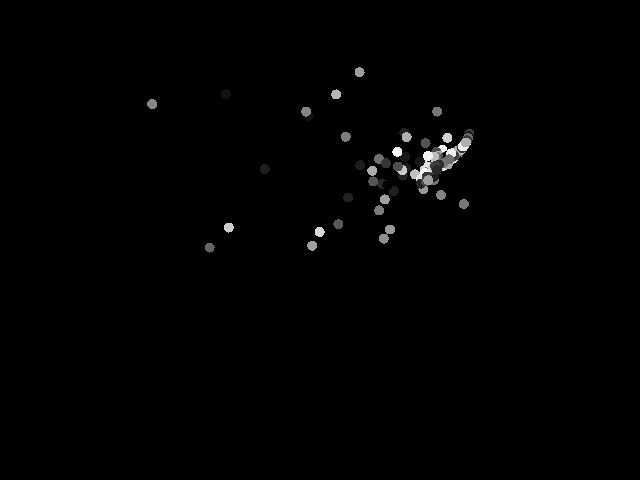
\includegraphics[width = 0.75\textwidth]{imgs/prace-s-objekty-1.png}
\end{center}

Rozeberme si jen letmo, k čemu vlastně došlo. Nejprve jsme definovali prázdné pole určené pro naše {\em entity}. Posléze jsme mu stanovili velikost a~celé pole jsme naplnili novými objekty {\em entit} (odborněji {\em instancemi}). V~poli se tedy nachází na každém místě jedna {\em entita}. Každou {\em entitu} poté ve~funkci \vyraz{draw()} k životu probouzíme prostřednictvím vnitřní funkce objektu {\em posunSeKeKurzoru()}. Všimněte si spuštění příkazu přes {\em tečkovou syntaxi}. Tím dochází k drobnému posunu každé okénko animace směrem ke kurzoru a~následnému vykreslení tvaru na plochu funkcí {\em kresli()}.



\oddil{Náhoda}

V minulé kapitole jsme hovořili o výrazu \vyraz{random()}, nyní se pokusíme poodhalit tajemství náhody v programování.

Proč má smysl v případě strojů vůbec hovořit o náhodě? Náhodu je z~pohledu výpočetní techniky třeba důsledně vnímat jako vnější vliv. V rámci počítačové logiky náhoda v podstatě neexistuje (není přípustná). Každý jev má svoji příčinu a~může mít svůj následek. Počítačové jazyky znají jen pojem takzvané pseudonáhodnosti.

Předložka pseudo- již nastiňuje určitou náhražku. Pseudonáhodnost je ve své podstatě strojová simulace náhody v čistě logickém prostředí. Náhodou pojmenováváme zpravidla jev, který nedokážeme pro jeho složitost předpovědět. Reálný svět vnímaný člověkem obsahuje takzvanou pravou náhodu, tedy to, co skutečně nelze vypozorovat.

Situace přenesení náhody do světa logického uvažování je velmi problematická proto, že člověk velmi těžko stroji popisuje fakt srozumitelnosti. Některá jednoduchá pravidla srozumitelná jsou, a jiná, z pohledu stroje \lnb obdobně jednoduchá, se lidskou optikou jeví již jako nesrozumitelná.

Pseudonáhodou člověk definuje takový výpočet, který samozřejmě vychází z logického výpočtu, člověk už ale nedokáže předpovědět jeho \lnb výsledek.

Konkrétní příklad, jak lze v {\em Processingu} vygenerovat pseudonáhodné číslo pomocí příkazu \vyraz{random()}, je:

\begin{lstlisting}
float nahodna = random(10);
println(nahoda);
\end{lstlisting}

Proměnná nazvaná {\em nahoda} nyní přijímá pseudonáhodnou hodnotu v rozmezí od nuly do deseti, již následně vytiskne do konzole. Druhý možný zápis je zadání dvou čísel, tedy rozsahu výsledné pseudonáhodné hodnoty.


\begin{lstlisting}
float nahodna = random(-10,20);
println(nahoda);
\end{lstlisting}

Jak je zřejmě pochopitelné, náhoda se nyní bude pohybovat v rozmezí čísla od minus deseti do dvaceti. To, co se vám konkrétně objeví v konzoli, nedokážu předpovědět, jedná se totiž o vaše pseudonáhodné číslo.

Tisk do konzole je samozřejmě jeden z možných výstupů. Náhodné číslo můžeme zobrazit graficky. Můžeme například animovat pozici elipsy na ploše:

\begin{lstlisting}
void setup(){
	size(640,480);
}


void draw(){
	background(255);
	fill(255);
	ellipse(width/2 + random(-5,5), height/2 + random(-5,5), 20, 20);
}
\end{lstlisting}


Spustíme-li tento program, uvidíme kmitající elipsu ve středu kreslicího plátna. Kmitání probíhá v rozmezí od minus pěti do plus pěti pixelů od středu v obou osách. Pro každé jednotlivé okénko se obměňuje nová pseudonáhodná hodnota, a tím dochází k animaci.

Příkazy {\em width} a {\em height} označují šířku a výšku plátna.




\pododdil{Perlinův šum}

Dalším možným strůjcem pseudonáhodně generované hodnoty je takzvaný {\em Perlinův šum} ({\em Perlin noise}). {\em Perlinův šum} je pojmenovaný po svém vynálezci Kenu Perlinovi a je velmi často využíván při generování přirozeně vypadajícího náhodného pohybu. Oproti příkazu \vyraz{random()} se {\em Perlinův šum} \vyraz{noise()} odvíjí plynule. Pro ilustraci si zde můžeme ukázat rozdíl mezi {\em Perlinovým šumem} a holým pseudonáhodným číslem.



\begin{lstlisting}
void setup(){
	size(640,480);
}


void draw(){
	background(255);
	fill(255);
	ellipse(width/2 + noise( frameCount/30.0 ), height/2 + noise( frameCount/10.0 ), 20, 20);
}
\end{lstlisting}

Pohyb obrazce bude nyní probíhat plynule ve zdánlivě nepředpovídatelných směrech. Příkaz \vyraz{noise()} předpokládá vstup, který určuje pozici v~šumu. {\em Perlinův šum} si můžeme představit jako neměnný graf, kterým můžeme procházet tam i zpět v závislosti na zaslané hodnotě. Jelikož do příkazu \vyraz{noise()} posíláme proměnnou hodnotu \vyraz{frameCount}, procházíme variacemi {\em Perlinova šumu}, výstupem bude vždy číslo v rozmezí nula až jedna.  \nlb Budeme-li potřebovat rozmezí jiné, můžeme šum vynásobit požadovaným rozsahem (jak je tomu v předchozím příkladu).

\bublina{Vyzkoušejte použití náhody a šumu ke kresbě různých prvků v~obraze, ovládejte rozsah pomocí myši.}



\chapter{Metody zobrazení}

\oddil{Renderovací mody}

Doposud jsme pracovali pouze s jednou metodou zobrazení. Standardně je {\em Processing} nastaven do dvourozměrného modu vykreslování, který se nazývá {\em JAVA2D}. Tento mod bude nastaven vždy, nezvolíte-li jiný mód. Další varianty jsou následující\poznamka{{\em Processing 2.0} přichází se značně pozměněným renderovacím enginem, varianty renderů {\em P2D} a {\em P3D} vzhledem ke zpětné kompatibilitě fungují, vnitřně je ovšem kompletně nahrazuje render {\em OPENGL}.}:

\begin{itemize}
\item[{\em JAVA2D}] Základní renderovací engine, který jsme používali doposud. Tento render podporuje dvoudimenzionální kresbu  a vyznačuje se dobrou kvalitou a precizností obrazu. Je obecně pomalejší než akcelerované rendery.

\item[{\em P2D}]  ({\em Processing 2D}) -- Akcelerovaný 2D render pro dvoudimenzionální kresbu, velmi výkonný pro operaci s jednotlivými pixely, postrádá ovšem přesnost {\em JAVA2D}. 

\item[{\em P3D}]({\em Processing 3D}) -- Akcelerovaný 3D render, používaný zejména pro webové aplikace. Přesnost je opět menší než u standardního renderu, dominuje rychlost.

\item[{\em OPENGL}] Rychlý 3D render využívající systém {\em OpenGL} pro grafické karty. {\em OpenGL} se hodí k vykreslování velkého množství objektů v relativně dobré kvalitě. Kvalita a hlavně rychlost velmi závisí na hardwaru.\poznamka{Ve verzi 1.0 render vyžaduje \vyraz{import} knihovny \odkaz{Knihovny}.}
\end{itemize}

Použití jednotlivých vykreslovacích prostředí lze provést ve funkci \vyraz{setup()} pomocí příkazu \vyraz{size()}:

\begin{lstlisting}
void setup(){

	//nastaveni renderu
	size(640, 480, P3D);

}

void draw(){

}
\end{lstlisting}

\oddil{3D zobrazení}

V případě renderů, které operují ve třetí dimenzi, v {\em Processingu} funguje řada příkazů podobně, jako jsme byli zvyklí v dvoudimenzionálním zobrazení. Největší změny se budou samozřejmě týkat zobrazení. V případě kresby primitivních obrazců v řadě případů přibude právě třetí rozměr.

Velmi ilustrativně je vidět rozdíl na příkazech \vyraz{point()} a \vyraz{line()}. U těchto příkazů jsme byli zvyklí zadávat dva parametry pro každou osu, tedy $X, Y$ pro bod, popřípadě čtyři parametry $X_{1}, X_{2}, Y_{1}, Y_{2}$ pro linku. K těmto parametrům v případě trojdimenzionálních zobrazení přibývá pro každý bod logicky ještě jeden parametr pro osu $Z$. 

\vfill



\begin{center}
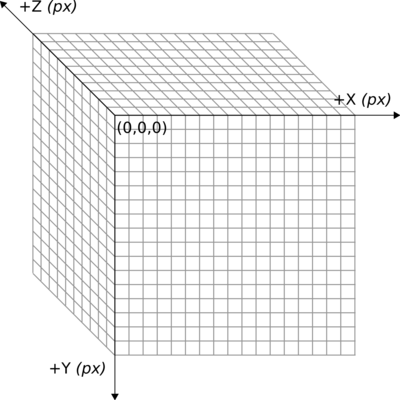
\includegraphics[width = 0.7\textwidth]{imgs/3d.png}
\end{center}

Osa $Z$ jakoby míří směrem k nám, negativní hodnoty se pak zobrazují ve větší vzdálenosti. Měrnou jednotkou je opět jeden pixel a hodnota nula pro všechny tři osy se nachází v levém horním rohu.

\pododdil{Kamera}

Zobrazení je zde pro ilustraci, ve skutečnosti probíhá v perspektivě, tedy se sbíhajícími se úběžníky. V prostoru se lze pohybovat pomocí nastavení pomyslné kamery funkcí \vyraz{camera()}.

\begin{lstlisting}
void setup() {

  // nastaveni 3D renderu
  size(300, 300, P3D);
  stroke(0);
  noFill();

    // prikaz pro nastaveni kamery 
    camera(-170.0, -135.0, 320.0, 50.0, 50.0, 0.0, 
    0.0, 1.0, 0.0);
}

//kresba
void draw() {

  background(255);
  
  box(120);
}
\end{lstlisting}

Příkaz \vyraz{camera()} nám nastaví pohled v trojrozměrné scéně. Příkaz přijímá poměrně hodně parametrů, rozeberme si, co všechno tyto parametry znamenají.

První tři parametry značí pozici kamery (nebo oka, chcete-li) ve třech rozměrech. Další tři parametry určují pozici bodu v prostoru, na který se kamera soustředí. Zbylé tři parametry udávají pozici nahoru ve tvaru vektoru.

Chceme-li se orientovat v prostoru tak, jak jsme byli zvyklí doposud, poslední tři hodnoty nastavíme jako $ 0,1,0$.

\begin{center}
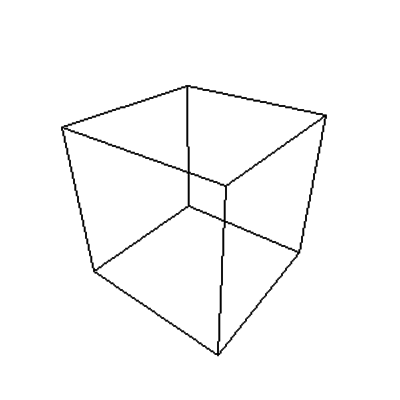
\includegraphics[width = 0.7\textwidth]{imgs/3dbox.png}
\end{center}

Kamera byla v předchozím příkladu nastavena ve funkci \vyraz{setup()}. Stejně tak lze nastavení obnovovat a měnit pro každé okénko. Shodně, jako jsme již animovali pohybující se objekt \odkaz{Animace}, můžeme animovat i kameru proměnou jednotlivých parametrů.

\pododdil{3D objekty}

V kontextu 3D zobrazení jsme zatím hovořili o bodu, lince a v předchozím příkladu jsme si zobrazili krychli příkazem \vyraz{box()}. Stejným příkazem \vyraz{box()} lze zkonstruovat i kvádr. Ten lze vytvořit pomocí tří parametrů pro rozměry ve třech osách $X,Y,Z$.

\bublina{Zkuste proměňovat hodnoty proměnné camera(), pozorujte jak se objekt proměňuje, ujistěte se, že rozumíte všem hodnotám zadávaným do funkce camera().}




Mezi další jednoduché tvary s možností zobrazení ve třech dimenzích patří dále koule -- \vyraz{sphere()} a úsečka ve třech dimenzích \vyraz{line()}. Její definice vyžaduje jediný parametr, ten určuje poloměr zobrazované koule. Nastavení počtu segmentů lze dále definovat příkazem \vyraz{sphereDetail()}. Pokud rozlišení nenastavíme, je standardně nastaveno na hodnotu 30, která klade nový segment každých 12 stupňů podle prostého výpočtu $360 / X = 12°$. $X$ je hodnota, kterou přijímá příkaz \vyraz{sphereDetail()}.


\begin{lstlisting}
void setup() {

  // nastaveni 3D renderu
  size(300, 300, P3D);
  sphereDetail(36);
  stroke(0,100);
  noFill();
  
    // prikaz pro nastaveni kamery 
    camera(-170.0, -135.0, 130.0, 0.0, 0.0, 0.0, 
    0.0, 1.0, 0.0);
}

//kresba
void draw() {
  background(255);
  sphere(120);
  
}
\end{lstlisting}


\begin{center}
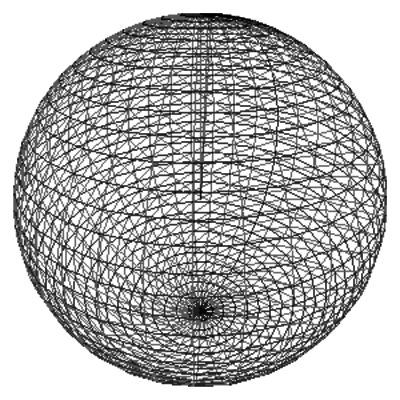
\includegraphics[width = 0.7\textwidth]{imgs/3dsphere.png}
\end{center}


Na veškeré objekty se vztahuje definice výplně a~kontury, tedy funkce \vyraz{fill()} a \vyraz{stroke()} \odkaz{Výplň a obrys}.

Tím výčet trojdimenzionálních objektů pomalu končí. Nic nám nebrání vytvářet kompozice pomocí bodů, krychlí a čar v prostoru. Složitější tvary lze stejně jako u dvoudimenzionálního zobrazení zkonstruovat pomocí \lnb vlastní definice tvaru, za použití takzvaných {\em vertexů} -- sadou příkazů \lnb \vyraz{vertex()} uzavřených do bloku \vyraz{beginShape()} a \vyraz{endShape()}.


Zde si musíme uvědomit, že konstrukce objektu po nás bude vyžadovat veliké množství informací. Pro přirovnání si vezměme konstrukci koule, v~případě vaší vlastní konstrukce byste museli každý z bodů definovat buď ručně, nebo lépe matematicky.

Metod, jak konstruovat 3D objekt, je mnoho a rozhodně by toto téma vystačilo na celého průvodce. Nyní nám postačí vědět, že je možné konstruovat i složitější tvary.

Další možností k tvorbě modelů je využít jiných programů (jako například otevřený software {\em Blender}) a následně pomocí rozšíření importovat externí modely přímo do {\em Processingu}\poznamka{K tomu lze použít externí knihovnu {\em ObjLoader} v {\em Processingu 1.x} anebo vestavěnou proměnnou {\em PShape} v {\em Processingu 2.x}.} \odkaz{Knihovny}.





\oddil{Transformace}

Vraťme se nyní zpět k dvěma rozměrům. {\em Processing} disponuje příkazy, které usnadňují práci s prostorem. Souhrnně se takové funkce dají nazvat transformace.


Uvedeme si zde základní koncepci práce s objekty v prostoru a jejich zobrazením. Nové funkce se jmenují \vyraz{translate()}, \vyraz{rotate()} a \vyraz{scale()}.

Představme si situaci, kdy potřebujeme pohybovat s jedním objektem. Jak jsme si ukázali již dříve \odkaz{Animace}, můžeme objektem pohybovat zadáváním jeho pozice.

Druhý způsob je v {\em Processingu} běžně využívaný a je o poznání dynamičtější, dovoluje nám totiž s objekty nejen pohybovat, ale měnit jejich rotaci nebo velikost.


\begin{center}
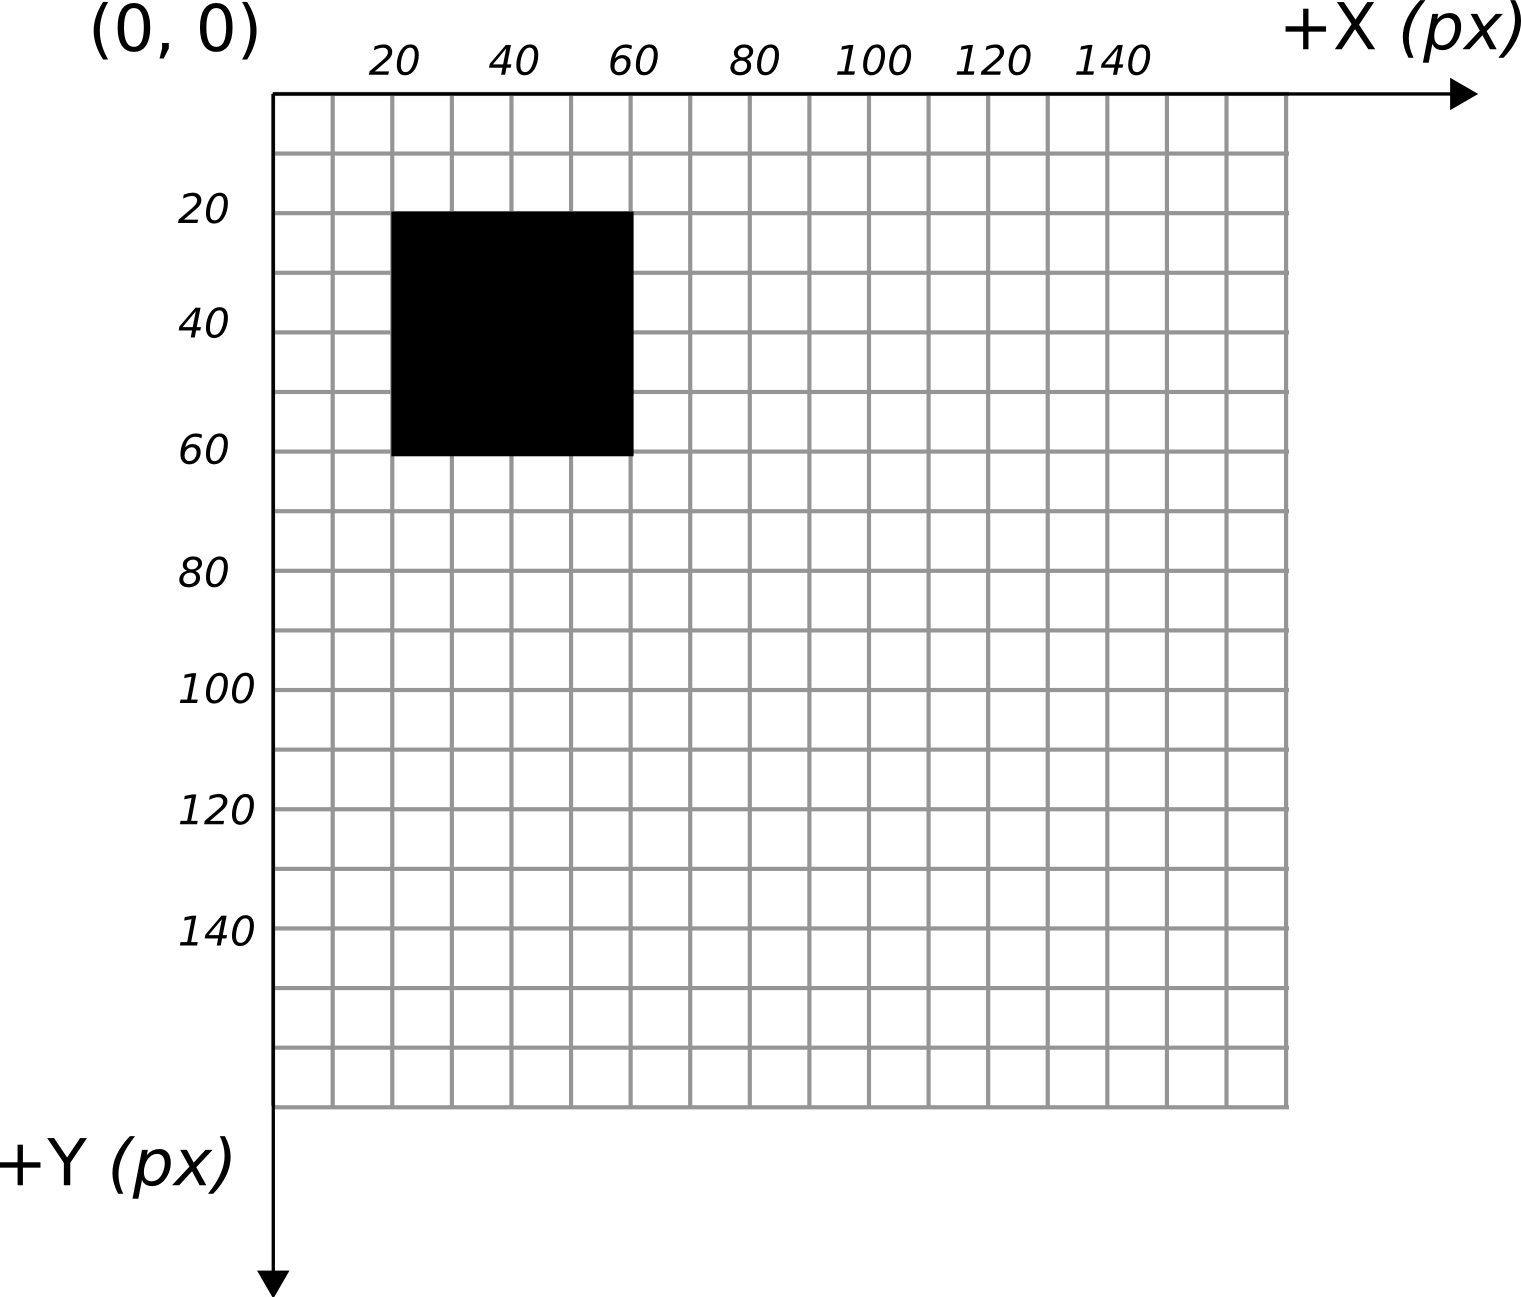
\includegraphics[width = 0.7\textwidth]{imgs/trans1.png}
\end{center}

Představme si nyní náš objekt jako čtverec na pozici $X=20, Y=20$ o~šířce a výšce dvaceti pixelů.



Jestliže budeme chtít přesunout čtverec o dvacet pixelů doprava a čtyřicet dolů, můžeme přičíst ke koordinátům tyto hodnoty:

\begin{lstlisting}
rect(20 + 20, 20 + 40, 40, 40);
\end{lstlisting}

Nebo můžeme použít transformaci posunu. Ta nám posune jakoby celou čtvrtkou papíru, na který kreslíme. Posun je vyjádřen funkcí \vyraz{translate()}.

\begin{lstlisting}
translate(20, 40);
rect(20, 20, 40, 40);
\end{lstlisting}

Čtverec se tak zobrazí na stejném místě, jako bychom docílili ručním posunem. Způsob je ale odlišný, ve skutečnosti jsme posunuli celým kreslicím plátnem.

\begin{center}
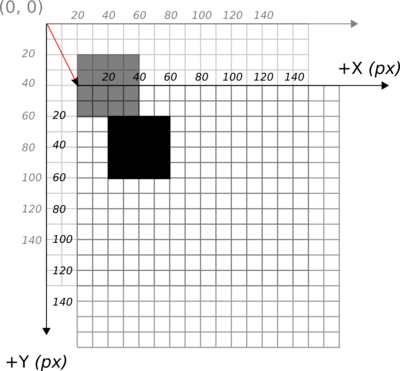
\includegraphics[width = 0.7\textwidth]{imgs/trans2.png}
\end{center}

Veškeré tvary, které nyní vykreslíme, budou posunuty o náš posun, tedy nemusíme posouvat všemi jednotlivými tvary zvlášť. Další operací, kterou můžeme provést, je rotace. Rotace vždy probíhá kolem bodu $X=0$, $Y=0$. Pomocí transformace můžeme přesunout objekt na požadované místo. K dalším operacím se nám budou hodit dva příkazy: \vyraz{pushMatrix()}, funkce, která započíná transformace, a \vyraz{popMatrix()}, která navrací plátno na původní místo. Při vícenásobných transformacích se nám může běžně stát, že budeme tyto bloky transformací vrstvit jednu do druhé. Exemplární rotaci si můžeme ukázat u podobného příkladu se čtvercem.

\bublina{Proměňte hodnoty ve funkci translate(), můžete použít například pozici myši mouseX a~mouseY a~pozorovat změny v kresbě.}

\begin{lstlisting}
void setup() {
  size(500, 500);
  fill(0);
  rectMode(CENTER);
}

void draw() {

  background(255);
  
  pushMatrix();  
  translate(150, 150);

  rotate( radians(45) );
  rect(20, 20, 100, 100);
  popMatrix();
}
\end{lstlisting}

Výsledkem bude čtverec otočený o $45°$. Příkaz \vyraz{rotate()} přijímá úhel \lnb v~radiánech, chceme-li otáčet o $45°$, musíme nejprve provést konverzi mezi úhly a radiány. Můžeme to provést snadno pomocí příkazu \vyraz{radians()}. Opačnou konverzi lze provádět pomocí příkazu \vyraz{degrees()}.




%\begin{center}
%
\includegraphics[width = 0.7\textwidth]{imgs/rot.png}
%\end{center}

Naše rotace v diagramu bude vypadat asi takto:

\begin{center}
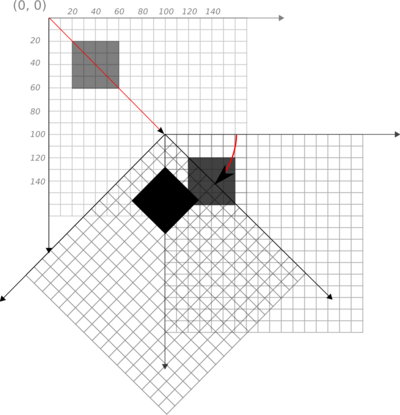
\includegraphics[width = 0.7\textwidth]{imgs/trans3.png}
\end{center}

První šipka znázorňuje posun, druhá šipka rotaci plátna. Osvojení si koncepce transformací je otázka zvyku, výhody toho, co se nyní jeví jako nepraktické, si uvědomíte možná později. Velikou výhodou transformací je například to, že si můžete definovat nový střed kresby, ke kterému se můžete vztahovat v relativních vzdálenostech.

Bez transformací se téměř vůbec neobejdete při kreslení ve třech rozměrech. Podobně jako u jiných příkazů i příkazy pro transformace zůstávají stejné. K funkci \vyraz{translate()} přibude třetí rozměr a funkce \vyraz{rotate()} se obohatí o rotace ve třech osách  \vyraz{rotateX()}, \vyraz{rotateY()}, \vyraz{rotateZ()}.


\pododdil{Použití transformací}

Jako souhrn všeho, co jsme nastínili v úvodu do transformací, se nyní pokusme analyzovat jeden z příkladů ze stránek {\em openprocessing.org} vytvořený Keithem Petersem.

\begin{lstlisting}
float[] x = new float[20];
float[] y = new float[20];
float segLength = 9;

void setup() {
  size(500, 500);
  smooth(); 
  strokeWeight(5);
  stroke(0, 100);
}

void draw() {
  background(225);
  dragSegment(0, mouseX, mouseY);
  for(int i=0; i<x.length-1; i++) {
    dragSegment(i+1, x[i], y[i]);
  }
}

void dragSegment(int i, float xin, float yin) {
  float dx = xin - x[i];
  float dy = yin - y[i];
  float angle = atan2(dy, dx);  
  x[i] = xin - cos(angle) * segLength;
  y[i] = yin - sin(angle) * segLength;
  segment(x[i], y[i], angle);
}

void segment(float x, float y, float a) {
  pushMatrix();
  translate(x, y);
  rotate(a);
  line(0, 0, segLength, 0);
  popMatrix();
}
\end{lstlisting}



V úvodu se nám objevují dvě pole, která představují soupis souřadnic. Další proměnná je definice délky jednoho segmentu. Ve funkci \vyraz{setup()} si můžeme povšimnout nového výrazu \vyraz{smooth()}.

Funkce \vyraz{smooth()} zajišťuje vyhlazení renderování, její protějšek je \lnb \vyraz{noSmooth()}. Vykonává jemnější obrazový výstup na úkor rychlosti.

Další funkcí, kterou jsme doposud neuvedli, je \vyraz{strokeWeight()}, ten definuje tloušťku čar a potažmo všech objektů. Šířka čáry je nastavena na~$1.0$. Funkce pracuje stejně jako výraz \vyraz{stroke()}, nastavuje tloušťku čáry pro \lnb všechny objekty níže.

Nakonec tu máme dvě definované funkce. První funkce {\em dragSegment()} přijímá hodnotu i ze smyčky a provádí trigonometrické matematické operace. Funkce začíná načtením minulé hodnoty souřadnic, kterou porovná \lnb s~hodnotami současnými a uloží výsledek. Zajímavá je funkce \vyraz{atan2()}. Ta~zjišťuje úhel v radiánech podle dvou hodnot v pořadí $Y$ a $X$. Zde jako vstupní hodnoty pro výpočet úhlu zadáváme rozdíl mezi současnými souřadnicemi segmentu pozicí minulého segmentu.

Podle zjištěného úhlu se dále modifikuje současná pozice za pomoci zpětného převedení na souřadnice přes \vyraz{cos()} a \vyraz{sin()}. Trigonometrii zde příliš rozvádět nebudu. Sinusovou křivku lze zkonstruovat lineárním přírůstkem ve funkci \vyraz{sin()}. Další goniometrické funkce jsou v {\em Processingu} \vyraz{asin()} a \vyraz{acos()}, šikovné pro práci s funkcemi jsou předdefinované hodnoty zlomku čísla $\pi$, \vyraz{PI}, \vyraz{HALFPI}, \vyraz{QUARTERPI}.

A konečně přicházejí na řadu naše transformace. Ve funkci {\em segment} dochází ke kresbě jednotlivých segmentů hada. Funkce přijímá tři argumenty, dva pro pozici $X$, $Y$ a jeden pro úhel $\alpha$. Sled transformací pomocí posunu a rotace již známe. 

\bublina{Transforma\-ce mohou být náročné na prostorovou představivost, nezoufejte při prvních nezdarech, po nějaké době a~cviku s~dvěma rozměry se můžete pokusit o transformace ve třetím rozměru.}
 




\chapter{Práce s daty}


Jak jsem v úvodu knihy \odkaz{Sketch} zmínil, adresář pro externí soubory se nazývá DATA. Tento adresář je umístěn přímo v adresáři projektu. Veškeré soubory, které do tohoto adresáře umístíme, budou programu dostupné.

V případě ukládání bude {\em Processing} zapisovat soubory do adresáře projektu. Všechny cesty k souborům budou tedy relativní.

Ukažme si nyní, jakým způsobem můžeme uložit a načíst vnější data do našeho programu.





\oddil{Ukládání informací}

Kresba do okna programu je jen jeden způsob výstupu programu. V určitém momentu budeme potřebovat zaznamenat obraz nebo jiná data pro další práci nebo archivaci. {\em Processing} umí ukládat data do rozmanitých formátů, při práci s obrazem se jedná o základní druhy bitmap a vektorového výstupu ve standardizovaném formátu {\em PDF}.

Při ukládání holých dat můžeme například využít prosté textové soubory, které se hodí při dalším zpracování pomocí {\em Processingu}. Velmi častý formát takového zápisu je takzvaný \slovnik{CSV}, což je v podstatě textový soubor obsahující data oddělená čárkou. Jeho velikost závisí na objemu dat. V~případě hieraticky strukturovaných dat je možné použít k uložení kupříkladu formát {\em XML}.


\pododdil{Ukládání obrazových dat}

Doposud jsme pracovali s obrazem, který je dočasný. Po zavření okna {\em Processingu} obraz nenávratně zmizí. K tomu, abychom z {\em Processingu} dostali obrazový výstup, potřebujeme kresbu uložit do souboru.

{\em Processing} umí ukládat různé formáty souborů. Nejběžněji budeme potřebovat uložit obrazová data jako rastrový obrázek. Formát obrázku si můžeme zvolit.

{\em Processing} umí ukládat rastrová data do následujících formátů:


\begin{itemize}
\item[TIFF]
nekomprimovaný obraz s příponou {\em *.tif, *.tiff}
\item[JPEG]
ztrátově komprimovaný obraz s příponou {\em *.jpg, *.jpeg}
\item[TARGA]
bezztrátově komprimovaný obraz (RLE) s příponou {\em *.tga}
\item[PNG]
bezztrátově komprimovaný obraz (DEFLATE) s příponou {\em *.png}

\end{itemize}

S některými formáty jste se již mohli setkat v minulosti. Jedná se \lnb o~standardní a rozšířené formáty pro uchovávání obrazových dat.

Uložení obrázku ze současného plátna se provádí příkazem \vyraz{save()}. Příkaz potřebuje znát cestu a koncovku souboru. Nenapíšeme-li plnou cestu, {\em Processing} data uloží přímo do adresáře naší sketche.

Nevíte-li, jakou koncovku souboru zvolit, doporučil bych vám vřele formát PNG. Takzvaný Portable Network Graphics je standard, který vyniká relativně malou velikostí a bezztrátovou kompresí dat. Vaše data tak budou uložena jedna ku jedné a můžete s nimi beze ztráty dále operovat. 

Samotné ukládání se provádí následujícím způsobem:

\begin{lstlisting} 
void setup(){
	size(640,480);
}

void draw(){
	background(255);
	line(mouseX,mouseY,pmouseX,pmouseY);

}


void mousePressed(){
	save("obrazek.png");
}

\end{lstlisting}


Příkaz \vyraz{save()} provede uložení obrazových dat okamžitě. Kdybychom vložili příkaz do kreslicí smyčky, {\em Processing} by se pokusil ukládat obrá\-zek šedesátkrát za vteřinu, což by se mu z důvodu relativní náročnosti operace zřejmě nepodařilo a byli bychom svědky zpomalení rychlosti ve vykreslování.

V příkladu tedy budeme ukládat obrázek jen po kliknutí myší.


Nyní si představme, že z nějakého důvodu potřebujeme zachytit plnou sekvenci po sobě jdoucích obrázků. Problém příkazu \vyraz{save()} je ten, že v~případě pevně zadané cesty bude stále přepisovat obrazovými daty tentýž soubor. Abychom uložili vícero obrázků, potřebujeme proměňovat cestu, kam {\em Processing} obrázky ukládá. Můžeme k tomu využít počitadlo nebo zvláštní příkaz  {\em Processingu} \vyraz{saveFrame()}:



\begin{lstlisting} 
void setup(){
	size(640,480);
}

void draw(){
	// kresba probehne zde

	save("obrazek" + nf( frameCount , 5 ) + ".png");
}

\end{lstlisting}

Využití počitadla je možné, ale trochu zdlouhavé. Všimněte si zde pouze způsobu, jakým číslujeme názvy souborů. Hodnota \vyraz{frameCount} se mění podle počtu vykreslených okének. Příkaz \vyraz{nf()} je zde z kosmetických důvodů, přidává pouze daný počet nul před naše počitadlo. Celý tento zápis se dá ovšem elegantně zkrátit příkazem \vyraz{saveFrame()}.


\begin{lstlisting} 
void setup(){
	size(640,480);
}

void draw(){
	// kresba probehne zde

	saveFrame("obrazek#####.png");
}

\end{lstlisting}

Příkaz \vyraz{saveFrame()} vyžaduje stejně jako příkaz \vyraz{save()} cestu k ukládanému souboru. Příkaz má ovšem navíc tu vlastnost, že vložíme-li do názvu souboru znaky křížku, {\em Processing} je rozpozná jako počet nul v počitadle okének.

\bublina{Vygenerujte si jednoduchou animaci za použití metody save-Frame(), zkuste ukládat jen na stisknutí tlačítka.}


\pododdil{Ukládání holých dat}

Ukládání informací do obrazu je jedna z možností. Někdy se nám může hodit uložit informace v jiném formátu. Řekněme, že potřebujeme uložit pozice myši pro pozdější animaci. Jistě bychom mohli uložit tuto informaci do série obrázků, z hlediska programování by to ovšem nebylo prozřetelné.

Konkrétní údaje o pohybu kurzoru známe. Můžeme je tedy zaznamenat například do nám již známého pole souřadnic. Pro tento účel si vytvoříme program, který bude umět zaznamenávat údaje o pohybu kurzoru do textového souboru. Předtím, než se pustíme do práce, je dobré si uvědomit, že text neobsahuje číselné informace. Vzpomínáte na kapitolu o základních datatypech \odkaz{Základní datatypy}? S textem, tedy ani textovým souborem, nelze manipulovat jako s čísly.

Při ukládání dat do textové podoby tudíž musíme mít již na mysli, jak je posléze budeme číst, a proto zvolíme vhodný formát pro ukládání. Vhodným formátem pro uchovávání informací v textové podobě je \slovnik{CSV}, Comma Separated Values. Jak z anglického názvu vyplývá, jedná se o hodnoty, které jsou odděleny čárkou. Pro naše potřeby budou stačit hodnoty dvě, pro osu X a osu Y našeho kurzoru.

Program si můžeme navrhnout následovně:

\begin{lstlisting}
float osaX[];
float osaY[];
int pocetHodnot = 300;

void setup(){

	size(640,480);
	osaX = new float[pocetHodnot];
	osaY = new float[pocetHodnot];
}


void draw(){

	osaX[frameCount] = mouseX;
	osaY[frameCount] = mouseY;

	if(frameCount >= pocetHodnot-1){
		ulozDoSouboru();
		exit();
	}
}

void ulozDoSouboru(){

	String[] holyText = new String[pocetHodnot];
	for(int i = 0 ; i < pocetHodnot; i++){
		holyText[i] = osaX[i]+", "+osaY[i];
	}
	
	saveStrings("soubor.csv",holyText);
}
\end{lstlisting}

Program je hotový. Rozeberme si doposud nevídané věci. Pole by nám měla být již srozumitelná, v tomto případě pouze používáme datatyp \vyraz{float}. Vytvořili jsme si dvě rozdílná pole pro dvě osy.

 Ve funkci \vyraz{draw()} nyní dochází k samotnému zápisu, a to pomocí již známé proměnné \vyraz{frameCount}. Hodnota je pokaždé zapsána na novou pozici. Následuje podmínka, která dříve novým příkazem \vyraz{exit()} ukončuje program. Podmínka je spuštěna pouze tehdy, máme-li již dostatečný počet zaznamenaných hodnot.
 
Podmínka navíc, dříve než ukončí celý program, spustí námi definovanou funkci pro uložení nashromážděných dat.

Tato funkce prostřednictvím smyčky převede číselné informace do textové podoby. Proměnné {\em osaX} a {\em osaY} funkce spojí dohromady pomocí znaménka plus spolu s čárkou a mezerou. Dále již následuje funkce {\em Processingu} \vyraz{saveStrings()}, která zajišťuje zápis pole textu do souboru. Koncovku jsem zde zvolil {\em *.csv}, ale je možné použít jakoukoli jinou, například {\em *.txt}.

 Podívejme se nyní do adresáře projektu (pomocí klávesy \klavesy{CTRL + k}). Soubor s názvem {\em soubor.csv} by měl být plný zaznamenaných hodnot.
 
 
 \begin{center}
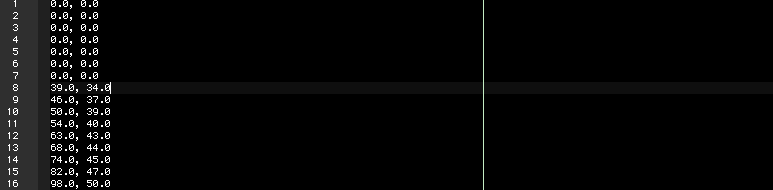
\includegraphics[width = 1\textwidth]{imgs/csv.png}
\end{center}

\bublina{Vyzkoušejte si ukládání různých proměňujících se hodnot, ověřte si po uložení v textovém editoru jak výsledný text vypadá.}

\pododdil{Tisk do PDF, ukládání vektorů}

Ukládat obrazové informace lze v rozmanitých formátech. Představme si, že jsme v {\em Processingu} navrhli grafiku, kterou bychom rádi tiskli v dobré kvalitě. Standardními postupy, tj. uložit obrazová data jako rastrový \nlb obrázek, docílíme kvality výsledného souboru jen v~rozměrech zadaných v~příkazu \vyraz{size()}. Sketch je primárně připravena pro zobrazení na obra\-zovce, a rozměry výsledného obrazu tedy většinou nepřesahuje rozměry naší obraz\-ovky.

Nic nám sice nebrání nastavit velikost sketche na několikanásobně větší plochu, než jakou naše obrazovka fyzicky disponuje, důmyslnějším řešením ovšem je uložit obrazová data jako vektorová ve formátu {\em PDF}. {\em PDF} je standardní formát pro práci s grafikou a předtiskovou přípravou a kromě rastrových obrazových dat může obsahovat i data vektorová.

 Největší výhodou vektorových dat je obecně škálovatelnost výstupních rozměrů. Jelikož jsou tvary vyjádřeny matematicky, celý obraz lze teoreticky tisknout v jakýchkoli rozměrech ve stejné kvalitě.
 
 Exportovat vektorová data lze v rozdílných formátech, dvourozměrná data budeme nejčastěji exportovat právě ve formátu {\em PDF} nebo {\em SVG}. Trojrozměrná data lze exportovat nejjednodušeji pomocí formátu {\em DXF}.
 
    {\em Processing} má funkci exportu do {\em PDF} již v sobě, pro jeho aktivaci ovšem musíme {\em Processingu} sdělit, že ji hodláme využít v naší sketchi.
    \newpage
 Postup při použití vykreslování do {\em PDF} je následující:
 
\begin{lstlisting} 

import processing.pdf.*;

void setup() {
  size(400, 400, PDF, "jmenoSouboru.pdf");
}

void draw() {

  //kreslit budeme zde
  line(0, 0, width/2, height);

  //a zde ukoncime program
  println("hotovo");
  exit();
}

\end{lstlisting}

V úvodu se objevil neznámý příkaz. Takzvaný \vyraz{import} značí načtení některých zvláštních funkcí rozšiřující funkce {\em Processingu}. Takové rozšíření se provádí pomocí takzvaných knihoven, o kterých se dočtete dále \odkaz{Knihovny}. 

Pro náš tisk je nyní důležité, že za příkazem \vyraz{import} se nachází právě cesta ke knihovně s {\em PDF} manipulacemi. Tuto cestu si nemusíme pamatovat, stejného výsledku docílíme i pomocí rozhraní {\em Processingu}. V~liště {\em Sketch $\rightarrow$ Import Library $\rightarrow$ PDF Export}.

V kódu je dále důležitá nová definice funkce \vyraz{size()}. Víme už, že tato funkce definuje rozměry sketche, v našem případě bude ovšem definovat rozměry výsledného {\em PDF} souboru. Za rozměry je dále nutné definovat vykreslovací prostředí {\em PDF} a jméno souboru, do kterého chceme zapisovat. Cesta k souboru je relativní, to znamená, že výsledný soubor se zobrazí přímo v adresáři naší sketche.

 Předchozí příklad vykreslil první okénko programu přímo do souboru, aniž by cokoli zobrazil a ukončil sám sebe. V dalším příkladu si ukážeme, jak vykreslovat v průběhu programu jinou fázi animace. K podobné manipulaci potřebujeme spustit a ukončit vykreslování do souboru na vyžádání.
 
\pagebreak
 
 \begin{lstlisting}
import processing.pdf.*;

boolean zaznam;

void setup() {
  size(400, 400);
}

void draw() {
  if (zaznam) {
    // vsimnete si ze #### bude nahrazeno cislem okenka
    beginRecord(PDF, "frame-####.pdf"); 
  }

  // kresleme zde
  background(255);
  line(mouseX, mouseY, width/2, height/2);

  if (zaznam) {
    endRecord();
	zaznam = false;
  }
}

// Use a keypress so thousands of files aren't created
void mousePressed() {
  zaznam = true;
}
 
 \end{lstlisting}
 
 
 Jak je na příkladu dobře vidět, zapisování do souboru spouštíme pomocí proměnné {\em zaznam}. Nahrávání vektoru do souboru začíná příkazem \vyraz{beginRecord()} a končí příkazem \vyraz{endRecord()}. Celou proceduru spouštíme prostřednictvím příkazu \vyraz{mousePressed()}.
 
 Pomocí předchozího způsobu uvidíme animaci vykreslovanou na plochu, kterou lze v daný moment uložit do jednotlivých souborů pojmenovaných podle čísla okénka, kdy kresba proběhla.
 
 Podobným způsobem, jakým lze zapsat vektorový obraz, je i metoda postupné kresby na jedno plátno, tedy do jednoho souboru.
 
\pagebreak
 
\begin{lstlisting}
import processing.pdf.*;

void setup() {
  size(400, 400);
  beginRecord(PDF, "platno.pdf");
}

void draw() {
  // nebudeme vykreslovat pozadi, abychom neprepsali nasi predchozi kresbu
  
  // kresba pomoci mysi
  line(mouseX, mouseY, width/2, height/2);
}

// ukoncime kresbu a program
void keyPressed() {
  if (key == 'q') {
    endRecord();
    exit();
  }
}
\end{lstlisting}

Takovým postupem lze kreslit opakovaně do jednoho souboru. Kresbu a celý program ukončíme pomocí funkce \vyraz{keyPressed()}, tedy klávesy \klavesy{Q}.

\bublina{Můžete vytvářet neomezeně složité tvary, zkuste jiné barvy výplně a~obrysů, otevřete vždy výsledný soubor a~ověřujete si výslednou podobu vektorové kresby. Zkuste kresbu načíst a~upravit v jiném vektorovém editoru (například otevřený Inkscape).}

\oddil{Načítání informací}

Za vnější informace lze v {\em Processingu} považovat vše, co není zdrojovým kódem {\em Processingu}. Takové informace můžeme souhrnně nazvat data. {\em Processing} umí nakládat s širokou škálou dat. Mezi ty nejčastěji používané bude patřit obrazová informace -- ať už v podobě rastrového, nebo vektorového obrazu. Mezi další vektorová data patří 3D modely nebo například záznamy z databází ve formátu {\em XML}, {\em CSV}, naprosto holé textové \lnb soubory atp. 

\pododdil{Načítání obrázků}

{\em Processing} ukládá obrázky do vnitřní paměti. Využívá k tomu speciální datatyp nazvaný \vyraz{PImage}. Pomocí tohoto datatypu si můžeme do našeho programu načíst externí obrazová data, se kterými můžeme dále pracovat. Načíst obrázek můžeme prostřednictvím příkazu \vyraz{loadImage()}. Příkaz bude očekávat jediný parametr, cestu k obrázku.

Zde je namístě připomenout \odkaz{Sketch}, že budeme-li potřebovat externí data, je dobré si je umístit přímo do adresáře naší sketche do složky s názvem {\em DATA}. Veškeré cesty, které budeme v kódu psát, budou k našim souborům relativní, to znamená, že přemístěním externích dat do našeho adresáře můžeme místo:

\begin{lstlisting}
PImage obrazek = loadImage("/obrazek/kdesi/v/hlubinach/adresaru/obrazek.jpg");
\end{lstlisting}

nyní napsat jednoduše:

\begin{lstlisting}
PImage obrazek = loadImage("obrazek.jpg");
\end{lstlisting}

Načítání obrázků provádíme zpravidla ve funkci \vyraz{setup()}. Tedy obrázek potřebujeme načíst pouze jednou za celý běh programu, a jelikož se jedná \\o poměrně náročnou operaci, je dobré ji v průběhu neopakovat příliš často.\poznamka{Jako například každé okénko animace, což je velmi obvyklá začátečnická chyba.}

Správné načítání obrázku do paměti a následné vykreslení bude vypadat takto:


\begin{lstlisting}
PImage obrazek;

void setup(){
  size(512,512);
  obrazek = loadImage("obrazek.jpg");
}

void draw(){
  image(obrazek,0,0);  
}
\end{lstlisting}

Zde stojí za povšimnutí funkce \vyraz{image()} -- touto funkcí můžeme zobrazovat jednotlivé obrázky. Druhé dva parametry udávají pozici levého horního rohu obrázku v obou osách. Pro změnu, například vycentrování obrázku, buď můžeme odečíst polovinu ze šířky obrázku:

\begin{lstlisting}
  image(obrazek, -obrazek.width/2, -obrazek.height/2);  
\end{lstlisting}

anebo použít funkci \vyraz{imageMode()}. Funkce dokáže proměnit chování příkazu \vyraz{image()}, možné hodnoty jsou {\em CORNER}, {\em CORNERS} a {\em CENTER}. \lnb {\em CORNER} je standardní chování příkazu \vyraz{image()}, místo odčítání poloviny šířky a výšky obrázku můžeme použít právě mod {\em CENTER}. Modus {\em CORNERS} se nám může hodit, potřebujeme-li definovat dva rohy místo šířky a~výšky vykreslovaného obrázku.

\bublina{Dejte si pozor na velikost obrázků, pracujte vždy raději s menšími.}

\pododdil{Načítání textových souborů}

Textové soubory jsou jednou z nejjednodušších cest, jak ukládat textové informace. To, že potřebujeme textový soubor, poznáme, jakmile budeme chtít pracovat s větším objemem textu, který se bude hromadit u definic proměnných.

Pokusme se nyní vrátit k předchozímu příkladu pro ukládání textových souborů \odkaz{Ukládání holých dat}. Zde jsem názorně ukázal, jak si uložit data generovaná {\em Processingem} pro další použití. Zkusme je tedy načíst. Pro připomínku, data vypadají následovně:

Na každém řádku jsou dvě hodnoty, které představují určitý záznam. Víme, že to je záznam pohybujícího se kurzoru, ale data mohou být opravdu cokoli. Co je pro nás důležité, je to, že jsme si uložili data v jednom tvaru, tzv. \vyraz{CSV}. Vždy se jedná o dvě hodnoty s desetinnou čárkou na jednom řádku oddělené čárkou a mezerou.

K samotnému načtení textových informací do paměti programu tak, \lnb abychom s textem mohli dále pracovat, použijeme stejně jako při ukládání pole řetězcových hodnot. To, co zní odpudivě, je ve skutečnosti docela prosté:

\begin{lstlisting}
String celyText[] = loadStrings("soubor.csv");
\end{lstlisting}

Příkazem \vyraz{loadStrings()} načteme veškeré textové informace ze souboru do obsahu naší proměnné. Proměnná musí být pole, pole typu \vyraz{String}.

Co příkaz \vyraz{loadStrings()} přesně udělá? Naplní celé pole hodnotami, každý jeden řádek přiřadí jedné přihrádce. Pro prosté ověření si nyní můžeme \lnb vytisknout obsah naší proměnné do konzole.

\begin{lstlisting}
println(celyText);

//////////// vysledek:
//[0] 0.0, 0.0
//[1] 0.0, 0.0
//[2] 0.0, 0.0
//[3] 0.0, 0.0
//[4] 0.0, 0.0
//[5] 0.0, 0.0
//[6] 0.0, 0.0
//[7] 39.0, 34.0
//[8] 46.0, 37.0
//[9] 50.0, 39.0
//... atd.
\end{lstlisting}

Tisk do konzole pomocí \vyraz{println()} je nastaven tak, že jestliže tiskne pole, zobrazí také hodnoty o místech, na kterých jsou informace v poli uložené.


\oddil{Operace s textem}

V minulé kapitole jsme úspěšně načetli hodnoty do paměti programu. Bude-me-li je nyní potřebovat k něčemu použít, musíme si rozmyslet, v jakém tvaru se nacházejí.

Navážeme-li na příklad z minulé kapitoly, naše proměnná má v sobě stále tytéž hodnoty a je ve tvaru pole {\em String[]}.

Kdyby se jednalo například o souvislý text -- báseň, patrně bychom ji chtěli zachovat v textové podobě. Jelikož jsou to ale čísla -- hodnoty, budou nám více platné pod datovým typem, se kterým budeme moci zacházet jako s číslem. Potřebujeme je tedy převést do čísel.

Převod z textových údajů do hodnot jiných typů se nazývá obecně {\em parsing}. Je to velmi častá procedura ve styku s daty třetí strany nebo i~s~daty, která jsme sami uložili.


\pododdil{Parsing, získávání hodnot z externích dat}

K převodu textu do užitelných hodnot můžeme využít následující postup. Budeme potřebovat zkonstruovat smyčku \odkaz{Smyčka}, která projde veškerý obsah načteného textového souboru a řádek po řádku naplní pole číselných hodnot odpovídajících hodnotám textovým. Celou tuto proceduru si můžeme uzavřít do jedné funkce.

Zopakujeme si načtení dat do pole. Program bude vypadat následovně:


\begin{lstlisting}
String celyText[];
float hodnotyX[];
float hodnotyY[];

void setup(){

	nactiTextDoHodnot();
	
	println(hodnotyX);
}


void nactiTextDoHodnot(String nazevSouboru){

	celyText = loadStrings(nazevSouboru);
	
	hodnotyX = new float[celyText.length];
	hodnotyY = new float[celyText.length];
	
	for(int i = 0 ; i < celyText.length ; i++){
		String radek = celyText[i];
		String[] hodnoty = splitTokens(radek,", ");
		
		hodnotyX[i] = parseFloat(hodnoty[0]);
		hodnotyY[i] = parseFloat(hodnoty[1]);
	}

}

//////////// vysledek:
//[0] 0.0
//[1] 0.0
//[2] 0.0
//[3] 0.0
//[4] 0.0
//[5] 0.0
//[6] 0.0
//[7] 39.0
//[8] 46.0
//... atd.
\end{lstlisting}

Projděme si, co se v programu stalo. Celá procedura zde spočívá ve~funkci nazvané {\em nactiTextDoHodnot()}. Jako argument do této funkce posíláme název souboru, který chceme načíst.

Jako první se spustí funkce, kterou již známe, \vyraz{loadStrings()}, ta naplní naše textové pole textem. Nyní je zapotřebí nastavit velikost číselných polí, pro přehlednost jsem zde vytvořil dvě pro každou osu. Jsou nazvány {\em hodnotyX} a~{\em hodnotyY}. Jejich budoucí velikost můžeme zjistit, bude stejná jako velikost textového pole. Přes příkaz {\em length} se můžeme dostat k délce jakéhokoli pole.

Nyní začneme s procházením textového pole, smyčka bude mít opět stejnou délku jako textové pole. Dočasná proměnná {\em radek} je zde spíše pro ilus\-traci, přiřazuje se k ní text pokaždé nového řádku.

Speciální textovou funkcí \vyraz{splitTokens()} rozdělíme řádek podle rozdělujících znaků. Víme, že náš zápis v souboru odděluje jednotlivé hodnoty čárkou a mezerou. Funkce \vyraz{splitTokens()} očekává první argument, text, který rozdělujeme, a jako druhý -- výčet znaků, které jej rozdělují, výsledně vrací nové pole rozděleného textu těmito znaky.

Poslední nevídaná funkce je \vyraz{parseFloat()}, ačkoli se nejedná přímo o~funk\-ci {\em Processingu}, ale přímo {\em Javy}, poslouží nám zde velmi dobře. Funkce \vyraz{parseFloat()} očekává text a převádí jej do čísla s desetinnou čárkou. Kdybychom měli čísla celá, mohli bychom použít také funkci \vyraz{parseInt()}, která dělá naprosto totéž s celými čísly.

Po načtení všech hodnot se program vrací do funkce \vyraz{setup()}, odkud byl spuštěn. Zde si můžeme pro ověření vytisknout hodnoty z číselného pole {\em hodnotyX}.

\bublina{Ujistěte se, že dobře rozumíte rozdílu mezi textovou informací a číselnou hodnotou v~programu. Zkuste vytvořit jinou strukturu dat a poté ji sami přečíst pomocí funkce parseInt() nebo parseFloat().}


\oddil{Vizualizace hodnot}

Vyjdeme-li z předchozího příkladu, máme již hodnoty zpracovány ve dvou číselných polích. Cesta k jejich následné vizualizaci je již prostá. Potřebujeme smyčku, která bude procházet celé pole a nakreslí podle hodnot patřičný tvar.

\begin{lstlisting}
String celyText[];
float hodnotyX[];
float hodnotyY[];

void setup(){

      size(640,480);
  
	nactiTextDoHodnot("soubor.csv");
	
}

// kresba probehne zde
void draw(){
  background(0);
  stroke(255, 127, 0);
  
  for(int i = 1 ; i < hodnotyY.length ; i++){
  
   line(hodnotyX[i], hodnotyY[i],
        hodnotyX[i-1], hodnotyY[i-1]); 
  
  }
}

void nactiTextDoHodnot(String nazevSouboru){

	celyText = loadStrings(nazevSouboru);
	
	hodnotyX = new float[celyText.length];
	hodnotyY = new float[celyText.length];
	
	for(int i = 0 ; i < celyText.length ; i++){
		String radek = celyText[i];
		String[] hodnoty = splitTokens(radek,", ");
		
		hodnotyX[i] = parseFloat(hodnoty[0]);
		hodnotyY[i] = parseFloat(hodnoty[1]);
	}

}
\end{lstlisting}

Výsledkem bude záznam pohybu myši, který může vypadat následovně:
\begin{center}
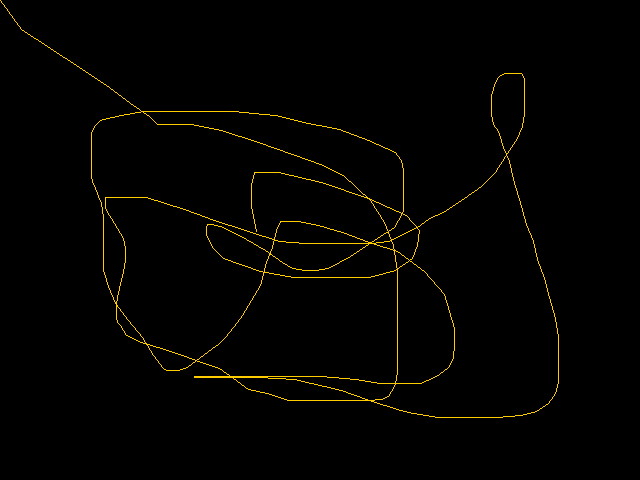
\includegraphics[width = 0.7\textwidth]{imgs/viz.png}
\end{center}

\bublina{Zkuste jiné hodnoty než pohyb myši, experimentujte s jinými způsoby zobrazení.}

Za povšimnutí zde stojí konstrukce linky \vyraz{line()}, která vždy spojuje koordináty z předchozího místa v našem poli s hodnotami současnými pomocí šikovného posunu o jednu pozici vzad {\em [i-1]}.


\vfill
\chapter{Rozšíření Processingu}
\oddil{Knihovny}

\pododdil{Vestavěné knihovny}
\index{vestavěné knihovny}

Ve {\em sketchbooku} se dále nacházejí\poznamka{Od verze 1.0.} veškerá rozšíření pomocí takzvaných knihoven neboli libraries. Ty jsou umístěny v adresáři {\em sketchbooku} ve~slož\-ce {\em libraries}. Knihovny jsou silným rozšířením celého jazyka a pokrývají \lnb mnoho možností nakládání s externími daty, zajišťují komunikaci se zařízeními, práci s videem, zvukem nebo s trojrozměrnými daty či vektorovým obrazem.


Knihovny jsou v podstatě moduly, které se zaměřují většinou pouze na jednu problematiku. Některé moduly umí například komunikovat se zapojenou kamerou nebo videem, jiné dovedou přenášet informace přes síť anebo komunikovat se zařízeními napojenými přes sériový port. Knihovna je sada příkazů, jež rozšiřuje samotný jazyk o nové možnosti.


Knihovnami se také dá dobře ilustrovat, k čemu uživatelé {\em Processingu} převážně programovací prostředí využívají. To sice nemusí být v žádném případě směrodatné pro vaši práci, může to být ovšem velmi inspirativní. Knihovny vám pomohou získat jistý přehled o kontextu užívání {\em Processingu}.

Knihovny se  nejobecněji dělí na dvě základní skupiny. Jednu tvoří inter\-ní knihovny {\em Processingu}, které přichází již nainstalované se softwarem, a knihovny vnější, vytvořené komunitou uživatelů. Veškeré nainstalované knihovny, které má Processing k dispozici, lze nalézt v liště pod tlačítkem {\em Sketch $\rightarrow$ Import Library}.


Výčet komunitních knihoven je již poměrně obsáhlý, pro ilustraci zde budeme hovořit jen o knihovnách vestavěných. Vestavěných knihoven je nepoměrně méně, jejich výčet se proměňuje relativně pomalu a jejich dokumentace je kvalitně zpracovaná:


\begin{itemize}
\item[Video] Základní rozhraní mezi {\em Apple Quicktime} a {\em Processingem}. U platformy Linux tato knihovna dlouhodobě nefunguje kvůli závislosti na propietárním softwaru, musíme tedy využít alternativy -- například implementaci nativní knihovny {\em GStreamer}.

\item[Network]
Zajišťuje základní síťovou + internetovou komunikaci. 

\item[Serial]
Podpora pro komunikaci se sériovými porty, externí zařízení \lnb typu {{\em (RS-232)}.

\item[PDF Export]
Knihovna pro export do {\em PDF}.

\item[OpenGL]
Technologie pro podporu {\em Java} implementace akcelerované grafiky prostřednictvím {\em JOGL}.

\item[Minim]
Využívá {\em JavaSound API} k snadné obsluze zvukového výstupu.

\item[DXF Export]
Knihovna pro exportování vektorových dat ve formátu {\em DXF} (Blender, Autocad, 3D).

\item[Arduino]
Knihovna určená pro komunikaci s {\em Arduinem}.

\item[JavaScript]
Nese metody pro komunikaci mezi {\em JavaScriptem} a processingovým appletem ve své webové podobě.

\item[SVG Import]
Knihovna pro načítání vektorové grafiky ve formátu {\em SVG} ({\em Inkscape}, {\em Adobe Illustrator}).

\item[XML Import]
Podpora načítání dat v {\em XML} formátu.
\end{itemize}

\newpage

Neříkají-li vám tyto zkratky nic, nevadí, jedná se většinou o datové standardy a typy zařízení, se kterými můžete pomocí knihoven pracovat. Každá z těchto knihoven má svoji dobrou dokumentaci: na stránkách projektu nebo přímo v tzv. {\em Examples}, příkladech pro každou knihovnu, lze tímto způsobem zobrazit základní nápovědu.

\bublina{Projděte si stránky processing.org a přečtěte si výčet knihoven, získáte lepší představu o možnostech rozšíření.}


\pododdil{Komunitní knihovny}

Instalace nových knihoven se zpravidla provádí umístěním adresáře s knihovnou do adresáře v našem {\em sketchbooku} nazvaném {\em libraries}. Pro kompletní výčet a popis všech komunitních knihoven zde není místo, je jich opravdu mnoho a další stále přibývají. Na aktuální stav se vždy můžete podívat na stránkách projektu {\em processing.org}.

\pododdil{Práce s knihovnou}

Jako poslední příklad si zde uvedeme práci s jednou externí knihovnou. S~jednou z interních jsme již pracovali dříve \odkaz{Tisk do PDF, ukládání vektorů}.

Dobrým příkladem funkční a použitelné knihovny pro {\em Processing} je \lnb knihovna {\em ControlP5} od Andrease Schlegela. Tato knihovna nám dovoluje snadno vytvářet interaktivní prvky jako tlačítka a různé typy táhel (sliderů) i~vstupních kolonek.

Knihovnu si nejprve musíme nainstalovat. Najdeme ji na webové adre\-se: {\em http://www.sojamo.de/libraries/controlP5}, anebo přímo na stránkách {\em processing.org}.

\vfill

\begin{center}
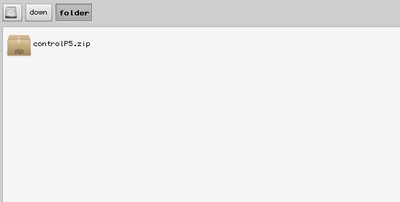
\includegraphics[width = 1\textwidth]{imgs/controlp5.png}
\end{center}

Soubor rozbalíme do adresáře {\em libraries} v našem {\em sketchbooku}, tj. adresáře, kam ukládáme naše sketche. Vnitřní struktura knihovny vypadá následovně:


\begin{center}
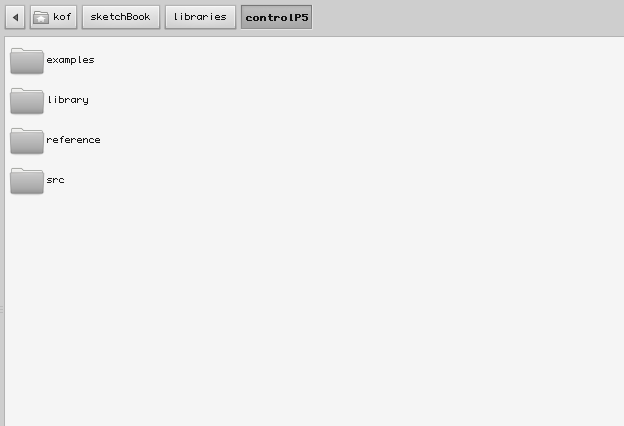
\includegraphics[width = 1\textwidth]{imgs/controlp52.png}
\end{center}

\newpage

Nejdůležitější složkou je v každé knihovně adresář {\em library}, zde se také nacházejí veškeré funkční prvky knihovny. Dále si můžeme všimnout dvou adresářů, {\em examples} a {\em reference}. Zde můžeme najít příklady použití i obsáhlou dokumentaci.

Máme-li spuštěný {\em Processing}, je nutné jej nyní restartovat.

Po spuštění je knihovna připravena k použití, přidat potřebné komponenty do kódu nyní můžeme buď ručně, nebo pohodlněji vybráním z nabídky: {\em Sketch $\rightarrow$ Import Library $\rightarrow$ controlP5}.

V kódu se nám zobrazí potřebný příkaz \vyraz{import} s náležitými komponenty z knihovny. Nyní si můžeme přečíst nápovědu nebo si projít jednotlivé příklady skrze nabídky: {\em File $\rightarrow$ Examples $\rightarrow$ Contributed Libraries $\rightarrow$ controlP5 $\rightarrow$ ControlP5controlEvent}.
Zobrazí se nám sketch:

 
\begin{lstlisting}
/**
 * ControlP5 ControlEvent
 * by andreas schlegel, 2009
 */
import controlP5.*;

ControlP5 controlP5;

int myColorRect = 200;
int myColorBackground = 100;

void setup() {
  size(400,400);
  frameRate(25);
  controlP5 = new ControlP5(this);
  controlP5.addNumberbox("n1",myColorRect,100,160,100,14).setId(1);
  controlP5.addNumberbox("n2",myColorBackground,100,200,100,14).setId(2);
  controlP5.addTextfield("n3",100,240,100,20).setId(3);
}

void draw() {
  background(myColorBackground);
  fill(myColorRect);
  rect(0,0,width,100);
}


void controlEvent(ControlEvent theEvent) {
  println("got a control event from controller with id "+theEvent.controller().id());
  if(theEvent.controller().id() == 1) {
    myColorRect = (int)(theEvent.controller().value());
  }else if(theEvent.controller().id() == 2){
    myColorBackground = (int)(theEvent.controller().value());
  }else if(theEvent.controller().id() == 3){
    println(theEvent.controller().stringValue());
  }
}
\end{lstlisting}

Veškeré příkazy by nám měly být vcelku povědomé, samozřejmě až na ty, které ovládají funkce knihovny {\em ControlP5}.

Všimněme si okamžitě objektu {\em ControlP5}, to je ústřední objekt při komunikaci s knihovnou. Objekt je vlastně třída, kterou jsme již rozebírali dříve \odkaz{Třída a objekt}. Vytvořením instance objektu z knihovny příkazem \vyraz{new} provážeme funkce knihovny s naším programem. Slovo \vyraz{this} referuje k našemu programu a říká knihovně, s čím bude své funkce propojovat. V podstatě ukazuje na nadřazenou (tzv. {\em super}) třídu samotné processingové aplikace (typu PApplet).

 Nyní již můžeme pomocí tečkové syntaxe vytvářet objekty z knihovny. V knihovně {\em ControlP5} je jich opravdu mnoho, zde si ukážeme pouze dva typy.  Příkazem {\em controlP5.addNumberbox} přidáváme objekt s hodnotou \lnb v~číselném formátu.
 
Objekt požaduje několik parametrů pro vytvoření: vlastní jméno, jméno proměnné, kterou bude ovládat, na konci definice proměnné také můžeme vidět speciální funkci  {\em setId(1)}, která nám bude identifikovat aktivitu daného prvku.

Tu můžeme detekovat pomocí nové funkce z knihovny nazvané {\em void controlEvent(ControlEvent theEvent)}. Ta zachytává veškeré dění s prvky a~posílá identifikační hodnotu, kterou posléze můžeme přečíst a napsat podle ní podmínku.

O kresbu prvků do smyčky \vyraz{draw()} se knihovna již postará sama.

\begin{center}
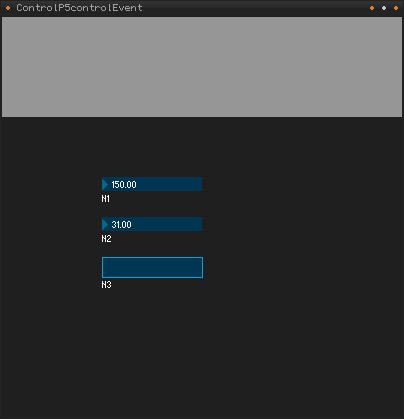
\includegraphics[width = 1\textwidth]{imgs/controlp53.png}
\end{center}

Výsledkem bude jednoduché {\em GUI}, grafické uživatelské rozhraní, pomocí kterého můžeme ovládat hodnoty v našem programu.


\bublina{Vyzkoušejte další příklady z~knihovny a zkuste i~knihovny další. Všech rozšíření je nyní přes 100 kusů, možností aplikace a kombinací je neomezeně.}


\newpage
\section{Poznávejte, experimentujte!}

Toto je konec úvodu do {\em Processingu}. Tento skromný průvodce vám chtěl pootevřít dveře do světa generované grafiky a programování jako takového. Další cesta bude již na vás.

Na závěr bych vám chtěl popřát hodně trpělivosti a odhodlání, obojího budete potřebovat nemálo. Výsledek své snahy ovšem můžete několikanásobně zúročit v další práci.

Hlavně se nebojte experimentovat, pocity frustrace nad nefungujícím kódem určitě vyváží uspokojení z vlastnoručně vytvořeného fungujícího programu. Odložte veškeré průvodce a zkoušejte stále nové postupy, i po několika letech zjistíte, že stojíte stále na začátku a můžete se učit novému. Čtěte kódy ostatních lidí a vyměňujte si programy, jejich zdroje \lnb -- vědomosti dále sdílejte s druhými lidmi.

Učte se vždy novému, nic není krásnějšího než na věci přicházet. A~když věcem rozumíte, nevlastněte je, předávejte vědomosti trpělivě dále.

\vfill


Aktualizovanou podobu tohoto průvodce můžete najít v elektronické verzi repozitáře {\em GIT} na serveru {\em GitHub} na adrese:\\
{\em https://github.com/K0F/processing\_1}

\begin{flushright}
{\em Kryštof Pešek, 12. května 2012}
\end{flushright}

\page


\addcontentsline{toc}{chapter}{Slovník}}

\printglossaries\thispagestyle{empty}


\addcontentsline{toc}{chapter}{Rejstřík}}

%\printglossaries
\printindex\thispagestyle{empty}


%\printindex
%
%
%
%\nocite{*}
%\printbibliography[title=Bibliografie]

\newpage

\


\thispagestyle{empty}

\vfill

\begin{itemize}
\item[]
Kryštof Pešek \\
\textbf{Processing Beta}

\item[]
Vydalo Nakladatelství Akademie múzických umění v Praze

\item[]
Redakce: Tomáš Pospiszyl, Andrea Slováková, Zdeňek Holý \\
Jazyková redakce: Jana Křížová, Olga Stehlíková \\ 
Tisková příprava: Jan Omasta \\
Obálka, grafická úprava a sazba: Kryštof Pešek


\item[]
Tisk NAMU \\
1. vydání \\
Praha 2013

\item[]
ISBN: 978-80-7331-224-4 \\
www.namu.cz, www.amu.cz 




\end{document}
